%%%%%% Run at command line, run
%%%%%% xelatex grad-sample.tex 
%%%%%% for a few times to generate the output pdf file
\documentclass[12pt,oneside,openright,a4paper]{cpe-thai-project}

\usepackage{enumitem}
% \usepackage{titlesec}

% \titleformat{\subsubsection}
% {}
% {\makebox[1in]{\bfseries}{\textbf\thesubsubsection}}{1em}\textbf{}
% \titlelabel{\llap{\makebox[1cm][l]{\thetitle}}\hspace*{25.4mm}}
% \titleformat{\section}
% {\bfseries\Large}{\thesection}{1pt}{\space}[\\]
% \titleformat{\section}[leftmargin]{\bfseries\Large}{\thesection}{1pt}{\space}[\\]
% % \titleformat{\section}[block]{\bfseries}{\thesection.}{1em}{}  
\usepackage{titlesec}

\titleformat{\subsection}{\bfseries\large}{\thesubsection}{1em}{}
\titlespacing*{\subsection}{\parindent}{2ex}{5em}

\titleformat{\subsubsection}{\bfseries\normalsize}{\thesubsubsection}{1em}{}
\titlespacing*{\subsubsection}{\parindent}{2ex}{5em}

\titleformat{\section}
  {\Large\bfseries}{\thesection}{1em}{}
\titlespacing*{\section}{\parindent}{*1.5}{0.75em}
\titlespacing{\subsubsection}{0em}{*1.5}{0.75em}
\titlespacing{\subsection}{0em}{*1.5}{0.75em}
\titlespacing{\section}{0em}{*1.5}{0.75em}
% \titleformat{\section}
% {\normalfont\Large\bfseries}{\thesection}{4pt}{\space}
% \titlespacing{\section}{0em}{0ex}{0em}
% \titlespacing*{\section}{\parindent}{0ex}{3em}

% \setlength{\parindent}{4pc} % exaggerated for the example
\usepackage{booktabs}
\usepackage{multirow}
\usepackage{arydshln}


\usepackage{polyglossia}
\usepackage{fontspec}
\setdefaultlanguage{thai}
\setotherlanguage{english}
% Set up Thai fonts
\setmainfont[%
    ItalicFont={Laksaman-Italic.otf},%
    BoldFont={Laksaman-Bold.otf},%
    BoldItalicFont={Laksaman-BoldItalic.otf},%
    Script=Thai,%
    Scale=MatchLowercase,%
    WordSpace=1.25,%
    Mapping=tex-text,%
]{Laksaman.otf}
\setlength\parindent{24pt}
%\newfontfamily\thaifont[Script=Thai,Scale=1.23]{TH Sarabun New}
%\defaultfontfeatures{Mapping=tex-text,Scale=1.23,LetterSpace=0.0}
%\setmainfont[Path=./Fonts/,Scale=1.23,LetterSpace=0,WordSpace=1.0,FakeStretch=1.0,Mapping=tex-text]{TH Sarabun New}
\XeTeXlinebreaklocale "th"
\XeTeXlinebreakskip = 0pt plus 0pt
\emergencystretch=10pt

%%%%%%%%%%%%%%%%%%%%%%%%%%%%%%%%%%%%%%%%%%%%%%%%%%%%%%%%%%%%%%%%%%%
% Customize below to suit your needs 
% The ones that are optional can be left blank. 
%%%%%%%%%%%%%%%%%%%%%%%%%%%%%%%%%%%%%%%%%%%%%%%%%%%%%%%%%%%%%%%%%%%
% First line of title
\def\disstitleone{Web Application for Automatic Nucleus Counting Immunofluorescence Tissue Biopsies}   
% Second line of title
\def\disstitletwo{}   
% Your first name and lastname
\def\dissauthor{Ms. Kanchayapond Seajoong}   % 1st member
%%% Put other group member names here ..
\def\dissauthortwo{Ms. Nichapat Nobnorb}   % 2nd member (optional)
\def\dissauthorthree{Mr. Wayu Ragwongsiri}   % 3rd member (optional)


% The degree that you're persuing..
\def\dissdegree{Bachelor of Science} % Name of the degree
\def\dissdegreeabrev{B.Sci} % Abbreviation of the degree
\def\dissyear{2022}                   % Year of submission
\def\thaidissyear{2565}               % Year of submission (B.E.)

%%%%%%%%%%%%%%%%%%%%%%%%%%%%%%%%%%%%%%%%%%%%
% Your project and independent study committee..
%%%%%%%%%%%%%%%%%%%%%%%%%%%%%%%%%%%%%%%%%%%%
\def\dissadvisor{Kharittha Jangsamsi, Ph.D.}  % Advisor
%%% Leave it empty if you have no Co-advisor
\def\disscoadvisor{Anyamanee Chaiprasongsuk, Ph.D.}  % Co-advisor
\def\disscoadvisorr{Paniti Achararit, Ph.D.}  % 3rd committee member (optional)
\def\disscoadvisortwo{Paniti Achararit, Ph.D.}  % 3rd committee member (optional)
\def\disscommitteetwo{Piyanit Wepulanon, Ph.D.}    % 5th committee member (optional) 

\def\worktype{Project} %%  Project or Independent study
\def\disscredit{3}   %% 3 credits or 6 credits


\def\fieldofstudy{Health Data Science} 
\def\department{Computer Engineering} 
\def\faculty{Engineering}

\def\thaifieldofstudy{วิทยาศาสตร์ข้อมูลสุขภาพ} 
\def\thaidepartment{วิศวกรรมคอมพิวเตอร์} 
\def\thaifaculty{วิศวกรรมศาสตร์}
 
\def\appendixnames{Appendix} %%% Appendices or Appendix

\def\thaiworktype{ปริญญานิพนธ์} %  Project or research project % 
\def\thaidisstitleone{เว็บแอปพลิเคชันสำหรับการตรวจนับนิวเคลียสจากภาพถ่ายเนื้อเยื่อจากการย้อมด้วยสารเรืองแสง}
%\def\thaidisstitletwo{หัวข้อปริญญานิพนธ์บรรทัดสอง}
\def\thaidissauthor{นางสาวกัญจน์ชยาภรณ์ แซ่จุง}
\def\thaidissauthortwo{นางสาวณิชาพัชร์ นบนอบ} %Optional
\def\thaidissauthorthree{นายวายุ รักษ์วงศ์สิริ} %Optional

\def\thaidissadvisor{ดร.คริษฐา แจ้งสามสี}
%% Leave this empty if you have no co-advisor
\def\thaidisscoadvisor{ดร.อัญมณี ชัยประสงค์สุข}
\def\thaidisscoadvisorr{ดร.ปณิธิ อัจฉราฤทธิ์}
\def\thaidisscoadvisortwo{ดร.ปณิธิ อัจฉราฤทธิ์}
\def\thaidissdegree{วิทยาศาสตรบัณฑิต}

% Change the line spacing here...
\linespread{1.15}

%%%%%%%%%%%%%%%%%%%%%%%%%%%%%%%%%%%%%%%%%%%%%%%%%%%%%%%%%%%%%%%%
% End of personal customization.  Do not modify from this part 
% to \begin{document} unless you know what you are doing...
%%%%%%%%%%%%%%%%%%%%%%%%%%%%%%%%%%%%%%%%%%%%%%%%%%%%%%%%%%%%%%%%


%%%%%%%%%%%% Dissertation style %%%%%%%%%%%
%\linespread{1.6} % Double-spaced  
%%\oddsidemargin    0.5in
%%\evensidemargin   0.5in
%%%%%%%%%%%%%%%%%%%%%%%%%%%%%%%%%%%%%%%%%%%
%\renewcommand{\subfigtopskip}{10pt}
%\renewcommand{\subfigbottomskip}{-5pt} 
%\renewcommand{\subfigcapskip}{-6pt} %vertical space between caption
%                                    %and figure.
%\renewcommand{\subfigcapmargin}{0pt}

\renewcommand{\topfraction}{0.85}
\renewcommand{\textfraction}{0.1}

\newtheorem{theorem}{Theorem}
\newtheorem{lemma}{Lemma}
\newtheorem{corollary}{Corollary}

\def\QED{\mbox{\rule[0pt]{1.5ex}{1.5ex}}}
\def\proof{\hspace{2em}{\itshape Proof: }}
\def\endproof{\hspace*{\fill}~\QED\par\endtrivlist\unskip}


% \makeatletter
% \newcommand\Xsubsubsection{\@startsection{subsubsection}{3}{\z@}%
%                                      {-2.25ex\@plus -1ex \@minus -.2ex}%
%                                      {1.5ex \@plus .2ex}%
%                                      {\normalfont\normalsize\bfseries\leftskip 5ex}}
% \renewcommand\subsubsection[1]{\Xsubsubsection{#1}\leftskip 5ex}
% \makeatother
%\newenvironment{proof}{{\sc Proof:}}{~\hfill \blacksquare}
%% The hyperref package redefines the \appendix. This one 
%% is from the dissertation.cls
%\def\appendix#1{\iffirstappendix \appendixcover \firstappendixfalse \fi \chapter{#1}}
%\renewcommand{\arraystretch}{0.8}
%%%%%%%%%%%%%%%%%%%%%%%%%%%%%%%%%%%%%%%%%%%%%%%%%%%%%%%%%%%%%%%%
%%%%%%%%%%%%%%%%%%%%%%%%%%%%%%%%%%%%%%%%%%%%%%%%%%%%%%%%%%%%%%%%

\usepackage{ragged2e}
\usepackage{booktabs}
\usepackage{caption}
\usepackage{indentfirst}
\usepackage{graphicx}
\usepackage{subcaption}
\usepackage{rotating}
\usepackage{colortbl}


\begin{document}

\pdfstringdefDisableCommands{%
\let\MakeUppercase\relax
}

\begin{center}
  
\includegraphics[width=2.8cm]{logo02.jpg}
\end{center}
\vspace*{-1cm}

\maketitlepage
\makesignaturepage 

%%%%%%%%%%%%%%%%%%%%%%%%%%%%%%%%%%%%%%%%%%%%%%%%%%%%%%%%%%%%%%
%%%%%%%%%%%%%%%%%%%%%% English abstract %%%%%%%%%%%%%%%%%%%%%%%
%%%%%%%%%%%%%%%%%%%%%%%%%%%%%%%%%%%%%%%%%%%%%%%%%%%%%%%%%%%%%%
\abstract

Nucleus counting is important in pathology as it helps in disease diagnosis and treatment development. Normally, pathologists count nuclei using Fluorescence Microscopy machines to image tissue stained with DAPI fluorescent dye and use the Columbus platform to count nuclei in the image automatically. However, the platform cannot accurately count and locate nuclei when they overlap, cluster together, or have indistinct shapes due to overlapping fluorescent dyes. This requires pathologists to manually count nuclei, which is time-consuming and prone to errors. Therefore, researchers studied the use of image processing techniques and deep learning, including Mask R-CNN, YOLO, and U-Net, to develop the best model for counting nuclei and compared them to develop a user-friendly web application. The YOLO model achieved the highest accuracy in nuclear counting, with an F1 score of 90.2 percent. The researchers hope that the developed web application will help reduce time and increase accuracy in nuclear counting.


\begin{flushleft}
\begin{tabular*}{\textwidth}{@{}lp{0.8\textwidth}}
\textbf{Keywords}: & Nucleus counting, Tissue immunofluorescence, Fluorochromes DAPI, Image Processing, Deep Learning, Web Application,
\end{tabular*}
\end{flushleft}
\endabstract

%%%%%%%%%%%%%%%%%%%%%%%%%%%%%%%%%%%%%%%%%%%%%%%%%%%%%%%%%%%%%%
%%%%%%%%%% Thai abstract here %%%%%%%%%%%%%%%%%%%%%%%%%%%%%%%%%
%%%%%%%%%%%%%%%%%%%%%%%%%%%%%%%%%%%%%%%%%%%%%%%%%%%%%%%%%%%%%%
% {\newfontfamily\thaifont{TH Sarabun New:script=thai}[Scale=1.3]
% \XeTeXlinebreaklocale "th_TH"	
% \thaifont
\thaiabstract
%ในร่างกายของมนุษย์ผิวหนังถือว่าเป็นอวัยวะที่มีขนาดใหญ่ที่สุดในร่างกาย โดยภายในเซลล์นั้นก็ถูกแบ่งออกเป็น 2 ส่วนหลัก ได้แก่ นิวเคลียสและไซโทรพลาสซึม ในการศึกษานี้จะให้ความสำคัญกับนิวเคลียส เนื่องจากนิวเคลียสมีหน้าที่ควบคุมการทำกิจกรรมต่าง ๆ ของเซลล์ รวมถึงยังมีหน้าที่เก็บรหัสพันธุกรรมของสิ่งมีชีวิต และมีหน้าที่ในการผลิตโปรตีน หากนิวเคลียสมีการเจริญเติบโตที่ปกติไปก็จะส่งผลต่อการเกิดโรคร้ายตามมาได้ ดังนั้นการนับจํานวนนิวเคลียสและปริมาณโปรตีนเป็นหนึ่งในขั้นตอนการทํางานในห้องปฎิบัติการ โดยการย้อมเนื้อเยื่อด้วยสารเรืองแสงแล้วถ่ายภาพด้วยเครื่อง Fluorescence Microscopy จะทําให้สามารถรู้ตําแหน่งและปริมาณของนิวเคลียสและโปรตีน ซึ่งจะได้ผลลัพธ์เป็นภาพถ่ายของเนื้อเยื่อที่มีสีระบุตําแหน่งที่แตกต่างกันไปตามการย้อมนั้น ๆ โดยสีย้อมที่ติดบริเวณนิวเคลียสจะเป็น DAPI ซึ่งเป็นสีนํ้าเงิน และสีย้อมที่ติดโปรตีนจะเป็น FITC เป็นสีเขียว และเนื่องจากนิวเคลียสจะทําหน้าที่ในการผลิตโปรตีน ทําให้ปริมาณของ
การนับจำนวนนิวเคลียสมีความสำคัญทางพยาธิวิทยา ช่วยในการวินิจฉัยโรคหรือพัฒนาการรักษา โดยปกติการนับจำนวนนิวเคลียสนักพยาธิวิทยาจะใช้เครื่อง Fluorescence Microscopy ถ่ายภาพเนื้อเยื่อที่ผ่านการย้อมด้วยสารเรืองแสง DAPI และใช้แพลตฟอร์ม Columbus นับจำนวนนิวเคลียสในภาพถ่ายอัตโนมัติแต่แพลตฟอร์ม Columbus ไม่สามารถนับจำนวนและแสดงตำแหน่งนิวเคลียสได้กรณีที่นิวเคลียสทับซ้อนกัน, เกาะกลุ่มติดกัน และมีรูปร่างที่ไม่แน่นอน นักพยาธิวิทยาจึงต้องนับจำนวนนิวเคลียสด้วยตนเอง ส่งผลให้ใช้เวลามากในการนับ และอาจเกิดความผิดพลาดได้ คณะผู้วิจัยจึงศึกษากระบวนการนับจำนวนนิวเคลียสด้วยการประมวลผลภาพ (Image Processing) และ การเรียนรู้เชิงลึก (Deep Learning) ประกอบด้วย Mask R-CNN, YOLO และ U-Net เพื่อพัฒนาแบบจำลองที่ดีที่สุดสำหรับนับจำนวนนิวเคลียส และนำแบบจำลองที่ดีที่สุดไปพัฒนาเว็บแอปพลิเคชันที่ง่ายต่อการใช้งาน จากผลการทดลองพบว่าการเรียนรู้เชิงลึกโดยใช้แบบจำลอง YOLO มีความแม่นยำในการนับนิวเคลียสสูงที่สุดคือค่า F1 score ที่ร้อยละ 90.2 
คณะผู้วิจัยหวังว่าเว็บแอปพลิเคชันที่ได้พัฒนาขึ้นมานี้จะสามารถช่วยลดเวลาและเพิ่มความแม่นยำในการนับจำนวนนิวเคลียสให้มีความแม่นยำเพิ่มมากขึ้น 

\begin{flushleft}
\begin{tabular*}{\textwidth}{@{}lp{0.8\textwidth}}
 & \\

\textbf{คำสำคัญ}: & การนับจำนวนนิวเคลียส, ภาพถ่ายเนื้อเยื่อจากการย้อมด้วยสารเรือง
แสง, สารเรืองแสง DAPI, การประมวลผลภาพ, การเรียนรู้เชิงลึก, เว็บแอปพลิเคชัน
\end{tabular*}
\end{flushleft}
\endabstract

%}

%%%%%%%%%%%%%%%%%%%%%%%%%%%%%%%%%%%%%%%%%%%%%%%%%%%%%%%%%%%%
%%%%%%%%%%%%%%%%%%%%%%% Acknowledgments %%%%%%%%%%%%%%%%%%%%
%%%%%%%%%%%%%%%%%%%%%%%%%%%%%%%%%%%%%%%%%%%%%%%%%%%%%%%%%%%%
\preface
การทำโครงงานครั้งนี้ประสบความสำเร็จลงได้ด้วยความช่วยเหลืออย่างดียิ่งของ ดร.คริษฐา แจ้งสามสี อาจารย์ที่ปรึกษา ตลอดจน ดร.อัญมณี ชัยประสงค์สุข และ ดร.ปณิธิ อัจฉราฤทธิ์ อาจารย์ที่ปรึกษาร่วม ที่กรุณาสละเวลาเพื่อให้คำปรึกษา เสนอแนะแนวทางที่ดี ให้ข้อมูล แนวความคิด และข้อเสนอแนะที่เป็นประโยชน์ ตลอดจนคอยติดตามดูแลเอาใจใส่ต่อการทำงานวิจัยนี้จนสำเร็จลุล่วงไปได้ดีด้วย คณะผู้วิจัยจึงขอกราบขอบพระคุณเป็นอย่างสูงมา ณ ที่นี้ 

ขอขอบพระคุณอาจารย์ ดร.อัญมณี ชัยประสงค์สุข ที่ให้ความช่วยเหลือในการเก็บรวบรวมข้อมูล และให้รายละเอียดของข้อมูลที่มีความสำคัญสำหรับการจัดทำงานวิจัยนี้ 

ขอขอบพระคุณ Dr. Sreenivas Bhattiprolu, Glenn Jocher, Matterport และ Sven P. Voigt สำหรับหลักการทำงาน ความรู้ และตัวอย่างการทำงานของอัลกอริทึมหรือแบบจำลอง รวมไปถึงตัวอย่างการนำไปใช้งานจริง

ขอขอบพระคุณคณะกรรมการ ผู้ให้ข้อมูล แนวคิด คำแนะนำ และข้อเสนอแนะที่เป็นประโยชน์ต่อการพัฒนางานวิจัยให้ดียิ่งขึ้น \\
%ขอขอบคุณภาควิชาวิศวกรรมคอมพิวเตอร์ มหาวิทยาลัยเทคโนโลยีพระจอมเกล้าธนบุรี ที่ให้การสนับสนุนนักศึกษาของภาควิชา ในการเข้าร่วมกิจกรรมอันเป็นประโยชน์นี้ \\
%ท้ายที่สุดนี้ โครงงานนี้อาจจะไม่สำเร็จเลยหากขาดผู้ปกครองที่ให้การสนับสนุน รวมทั้งเพื่อน ๆ พี่ ๆ ในภาควิชา ที่คอยเป็นกำลังใจสำคัญเสมอมา

%%%%%%%%%%%%%%%%%%%%%%%%%%%%%%%%%%%%%%%%%%%%%%%%%%%%%%%%%%%%%
%%%%%%%%%%%%%%%% ToC, List of figures/tables %%%%%%%%%%%%%%%%
%%%%%%%%%%%%%%%%%%%%%%%%%%%%%%%%%%%%%%%%%%%%%%%%%%%%%%%%%%%%%
% The three commands below automatically generate the table 
% of content, list of tables and list of figures
\tableofcontents                    
\listoftables
\listoffigures                      

%%%%%%%%%%%%%%%%%%%%%%%%%%%%%%%%%%%%%%%%%%%%%%%%%%%%%%%%%%%%%%
%%%%%%%%%%%%%%%%%%%%% List of symbols page %%%%%%%%%%%%%%%%%%%
%%%%%%%%%%%%%%%%%%%%%%%%%%%%%%%%%%%%%%%%%%%%%%%%%%%%%%%%%%%%%%
% You have to add this manually..
%\listofsymbols
%\begin{flushleft}
%\begin{tabular}%{@{}p{0.07\textwidth}p{0.7\textwidth}p{0.1\textwidth}}
%\textbf{SYMBOL}  & & \textbf{UNIT} \\[0.2cm]
%$\alpha$ & Test variable\hfill & m$^2$ \\
%$\lambda$ & Interarival rate\hfill &  jobs/second\\
%$\mu$ & Service rate\hfill & jobs/second\\
%\end{tabular}
%\end{flushleft}
%%%%%%%%%%%%%%%%%%%%%%%%%%%%%%%%%%%%%%%%%%%%%%%%%%%%%%%%%%%%%%
%%%%%%%%%%%%%%%%%%%%% List of vocabs & terms %%%%%%%%%%%%%%%%%
%%%%%%%%%%%%%%%%%%%%%%%%%%%%%%%%%%%%%%%%%%%%%%%%%%%%%%%%%%%%%%
% You also have to add this manually..
%\listofvocab
%\begin{flushleft}
%\begin{tabular}{@{}p{1in}@{=\extracolsep{0.5in}}l}
%DAPI    & 4’,6-diamidino-2-phenylindole \\
%mRNA    & Messenger Ribonucleic Acid
%CLAHE   & Contrast Limited Adaptive Histogram Equalization \\
%R-CNN   & Region-besed Convolutional Nueral Network

%\end{tabular}
%\end{flushleft}

%\setlength{\parskip}{1.2mm}

%%%%%%%%%%%%%%%%%%%%%%%%%%%%%%%%%%%%%%%%%%%%%%%%%%%%%%%%%%%%%%%
%%%%%%%%%%%%%%%%%%%%%%%% Main body %%%%%%%%%%%%%%%%%%%%%%%%%%%%
%%%%%%%%%%%%%%%%%%%%%%%%%%%%%%%%%%%%%%%%%%%%%%%%%%%%%%%%%%%%%%%


\chapter{บทนำ}

\section{ที่มาและความสำคัญ}
%การพัฒนาเทคโนโลยีในยุคดิจิทัลนี้ได้เริ่มเข้ามามีบทบาทสำคัญต่อการพัฒนาสิ่งต่าง ๆ ให้มีความทันสมัยและสามารถอำนวยความสะดวกในชีวิตประจำวันของเราให้สามารถดำเนินชีวิตได้ง่ายมากยิ่งขึ้น ตลอดจนมีการนำเอาเทคโนโลยีระดับสูงมาประยุกต์ใช้ในการวิจัยกันอย่างแพร่หลาย ซึ่งในทางการแพทย์ก็มีการนำเทคโนโลยีมาประยุกต์ใช้เช่นเดียวกัน อาทิเช่น งานวิจัยที่เกี่ยวกับความหลากหลายทางชีวภาพในมนุษย์ ตัวอย่างเช่น การตรวจนับนิวเคลียสจากภาพถ่ายเนื้อเยื่อจากการย้อมด้วยสารเรืองแสง เป็นต้น

%ร่างกายของมนุษย์ผิวหนังถือว่าเป็นอวัยวะที่ใหญ่ที่สุดในร่างกายของเรา โดยมีน้ำหนักรวมกันประมาณ 6 ปอนด์ หรือคิดเป็น 7\% ของน้ำหนักตัว ผิวหนังประกอบด้วย 3 ชั้น คือ หนังกำพร้า หนังแท้ และชั้นใต้ผิวหนัง ซึ่งภายในผิวหนังจะประกอบไปด้วยเนื้อเยื่อที่มีการรวมตัวกันของเซลล์อยู่เป็นจำนวนมาก ซึ่งมีจำนวนมากถึง 52,000 ล้านเซลล์\cite{cell1} 
นิวเคลียสเป็นส่วนประกอบหนึ่งของเซลล์ หน้าที่สำคัญของนิวเคลียสจะเป็นตัวควบคุมการทำกิจกรรมต่าง ๆ ของเซลล์ \cite{cell2} เป็นหน่วยที่ใช้เก็บรหัสพันธุกรรม และมีหน้าที่ในการผลิตโปรตีน\cite{cell3} การนับจำนวนนิวเคลียสจึงมีความสำคัญทางพยาธิวิทยา มีส่วนช่วยในการวินิจฉัยโรคหรือพัฒนาการรักษา โดยการนับจำนวนนิวเคลียสและปริมาณโปรตีนเป็นหนึ่งในขั้นตอนการทำงานในห้องปฎิบัติการ โดยการย้อมเนื้อเยื่อด้วยสารเรืองแสงแล้วถ่ายภาพด้วยเครื่อง Fluorescence Microscopy ซึ่งจะได้ผลลัพธ์เป็นภาพถ่ายของเนื้อเยื่อที่มีสีระบุตำแหน่งที่แตกต่างกันไปตามการย้อมนั้น ๆ โดยสีย้อมที่ติดบริเวณนิวเคลียสจะเป็น DAPI ซึ่งเป็นสีน้ำเงิน และสีย้อมที่ติดโปรตีนจะเป็น FITC เป็นสีเขียว และเนื่องจากนิวเคลียสจะทำหน้าที่ในการผลิตโปรตีน ทำให้ปริมาณของนิวเคลียสที่มีจำนวนมากในภาพถ่ายเนื้อเยื่อจากการย้อมด้วยสารเรืองแสงก็จะทำให้มีปริมาณของโปรตีนที่มากตามไปด้วย 

Columbus \cite{11} เป็นแพลตฟอร์มที่ช่วยในการวิเคราะห์ภาพและนับจำนวนนิวเคลียสที่ทำงานได้อย่างแม่นยำเมื่อรูปเนื้อเยื่อที่ถูกย้อมสีนั้นมีนิวเคลียสที่แยกตัวกันเป็นเซลล์เดี่ยวอย่างชัดเจน และมีลักษณะของเซลล์ที่เป็นรูปร่างคล้ายคลึงกัน นักพยาธิวิทยาจึงใช้โปรแกรมนี้ในการช่วยนับจำนวนของนิวเคลียสในเนื้อเยื่อนั้น ๆ ได้ แต่เมื่อเปลี่ยนเป็นภาพถ่ายเนื้อเยื่อจากการย้อมด้วยสารเรืองแสงที่ซ้อนทับกันหลายชั้น จะไม่สามารถใช้งาน Columbus ได้ซึ่งชุดข้อมูลภาพถ่ายเนื้อเยื่อจากการย้อมด้วยสารเรืองแสงที่คณะผู้วิจัยให้ความสนใจนั้นจะมีปัญหาเรื่องการซ้อนทับกัน ลักษณะของนิวเคลียสมีการรวมกลุ่มกันและติดกันเป็นจำนวนมาก และส่วนใหญ่นิวเคลียสมีลักษณะรูปร่างที่ไม่แน่นอน นอกจากนี้บริเวณขอบของนิวเคลียสยังเบลอไม่ชัดเจนส่งผลให้สายตาของมนุษย์ไม่สามารถแยกนิวเคลียสออกจากกันได้แบบทันที ต้องใช้เวลาวิเคราะห์ผลที่ค่อนข้างนาน และผลลัพธ์ที่ได้อาจจะไม่แม่นยำหรือคลาดเคลื่อนได้

จากการศึกษาพบว่ามีการนำเทคโนโลยีมาใช้นับจำนวนและระบุตำแหน่งของนิวเคลียส ตัวอย่างเช่น งานวิจัยของ Gyuhyun Lee และคณะ \cite{28} ศึกษาหาตำแหน่งของนิวเคลียส จากภาพถ่ายเรืองแสงจากกล้องจุลทรรศน์ของเนื้อเยื่อผิวหนังที่ถูกย้อมด้วยสารเรืองแสง DAPI, งานวิจัยของ Daniel Jimenez-Carretero และคณะ \cite{29} ศึกษาการเรียนรู้เชิงลึกที่ทําให้สามารถจําแนกรูปภาพแบบที่มีความซับซ้อนได้อย่างมีประสิทธิภาพ และใช้โครงข่ายประสาทแบบคอนโวลูชันในการทำนายความเป็นพิษของยาจากภาพนิวเคลียสที่ถูกย้อมด้วยสารเรืองแสง DAPI และ งานวิจัยของ Wafaa Rajaa Drioua และคณะ \cite{yolopaper} ศึกษาหานิวเคลียสซึ่งจําเป็นสําหรับการระบุลักษณะของมะเร็ง โดยนำการเรียนรู้เชิงลึกมาใช้เพื่อแยกจำนวนนิวเคลียส จากภาพถ่าย breast cancer histopathology จากการศึกษางานวิจัยดังที่กล่าวมาพบว่าส่วนใหญ่จะให้ความสนใจกับการนับจำนวนนิวเคลียสจากแบบจำลองการเรียนรู้เชิงลึกซึ่งผลลัพธ์ที่ได้เป็นที่น่าพอใจ แต่ด้วยรูปชุดข้อมูลของงานวิจัยเหล่านี้เป็นภาพเซลล์เดี่ยวที่ไม่ซ้อนทับกัน คณะผู้วิจัยจึงนำแนวทางการเรียนรู้เชิงลึกมาเป็นตัวพัฒนาแบบจำลองสำหรับนับจำนวนนิวเคลียสที่มีการซ้อนทับกันต่อไป

ดังนั้นจากการศึกษาข้างต้น ทำให้คณะผู้วิจัยเล็งเห็นถึงปัญหาในการนับจำนวนนิวเคลียสจากภาพถ่ายเนื้อเยื่อจากการย้อมด้วยสารเรืองแสงที่มีการซ้อนทับกัน จึงมีแนวคิดที่จะพัฒนาแบบจำลองที่สามารถตรวจจับตำแหน่งของนิวเคลียสและนับจำนวนของนิวเคลียสและพัฒนาให้ออกมาเป็นเว็บแอปพลิเคชันที่สามารถใช้นับจำนวนนิวเคลียสจากภาพถ่ายเนื้อเยื่อจากการย้อมด้วยสารเรืองแสงได้อัตโนมัติ เพื่อช่วยลดเวลาในการนับจำนวนนิวเคลียสของนักพยาธิวิทยา และเพื่อเพิ่มความแม่นยำในการนับจำนวนนิวเคลียสให้มีความแม่นยำมากยิ่งขึ้น

%การศึกษาการนับจำนวนนิวเคลียสเป็นหนึ่งในขั้นตอนการทำงานในห้องปฎิบัติการ โดยการนับนิวเคลียสนั้นทำเพื่อหาปริมาณของนิวเคลียสต่อขนาดชิ้นเนื้อที่เราต้องการศึกษา เพื่อเป็นการดูการเจริญเติบโตของตัวนิวเคลียสเองหรือเพื่อเป็นการวินิจฉัยโรคและการรักษาโรคต่อไป ซึ่งทางกลุ่มมีความสนใจเกี่ยวกับการนับจำนวนนิวเคลียสใน Immunofluorescence Tissue เพราะว่าจำนวนของนิวเคลียสสามารถส่งผลต่อปริมาณของโปรตีนได้ เนื่องจากนิวเคลียสจะทำหน้าที่ในการผลิตโปรตีน ส่งผลให้ Immunofluorescence Tissue ที่มีจำนวนของนิวเคลียสที่มากก็จะทำให้มีปริมาณของโปรตีนที่มากตามไปด้วย 

%การจะนับปริมาณของนิวเคลียสและโปรตีนที่สนใจใน Immunofluorescence Tissue ด้วยวิธีการมาตรฐานจะใช้วิธีการย้อมสารเรืองแสงลงไปบนเนื้อเยื่อ แล้วถ่ายภาพด้วยเครื่อง Fluorescence Microscopy ซึ่งจะได้ผลลัพธ์เป็นภาพถ่ายของนิวเคลียสที่มีสีที่แตกต่างกันไปตามการย้อมนั้น ๆ โดยสีของนิวเคลียสจะเป็นสีน้ำเงินและสีของโปรตีนจะเป็นสีเขียว ซึ่งการจะนับปริมาณของนิวเคลียสและโปรตีนในกรณีที่เป็นภาพ Single Cell จะสามารถใช้งานโปรแกรม Columbus \cite{11} เพื่อช่วยทำการนับได้ แต่เมื่อเปลี่ยนเป็นภาพของ Immunofluorescence Tissue จะไม่สามารถใช้งานโปรแกรม Columbus ได้ เพราะเกิดการทับซ้อนกันของนิวเคลียส เช่น นิวเคลียสทรงกลม 2 อันซ้อนทับกันไม่สนิท ทำให้รูปทรงที่มองเห็นไม่เป็นทรงกลมจริงๆ ส่งผลให้โปรแกรม Columbus ไม่สามารถใช้งานได้ 

%ซึ่งชุดข้อมูลที่เราสนใจนั้นจะมีปัญหาเรื่องการเกาะกลุ่มและซ้อนทับกันอย่างมากจนไม่สามารถแยกได้ด้วยตาเปล่าได้ รวมถึงรูปทรงของนิวเคลียสมีความไม่แน่นอน อาจเป็นทรงรีเรียวยาวหรือทรงรีใกล้เคียงทรงกลม ดังรูปภาพที่ \ref{fig:intro} นอกจากนี้ ด้วยวิธีการย้อมสีนั้นอาจทำให้เกิดการเบลอของภาพนิวเคลียสได้ ซึ่งส่งผลกับการหาขอบของนิวเคลียสที่เป็นขั้นตอนหนึ่งในการนับจำนวนนิวเคลียสได้ 

%เราจึงให้ความสนใจที่จะพัฒนาเว็บแอปพลิเคชันที่สามารถใช้นับจำนวนนิวเคลียสจากภาพเนื้อเยื่อได้อัตโนมัติ เพื่อเพิ่มความสะดวกสบายและความแม่นยำในการนับจำนวนนิวเคลียส 

%\begin{figure}[!h]\centering
%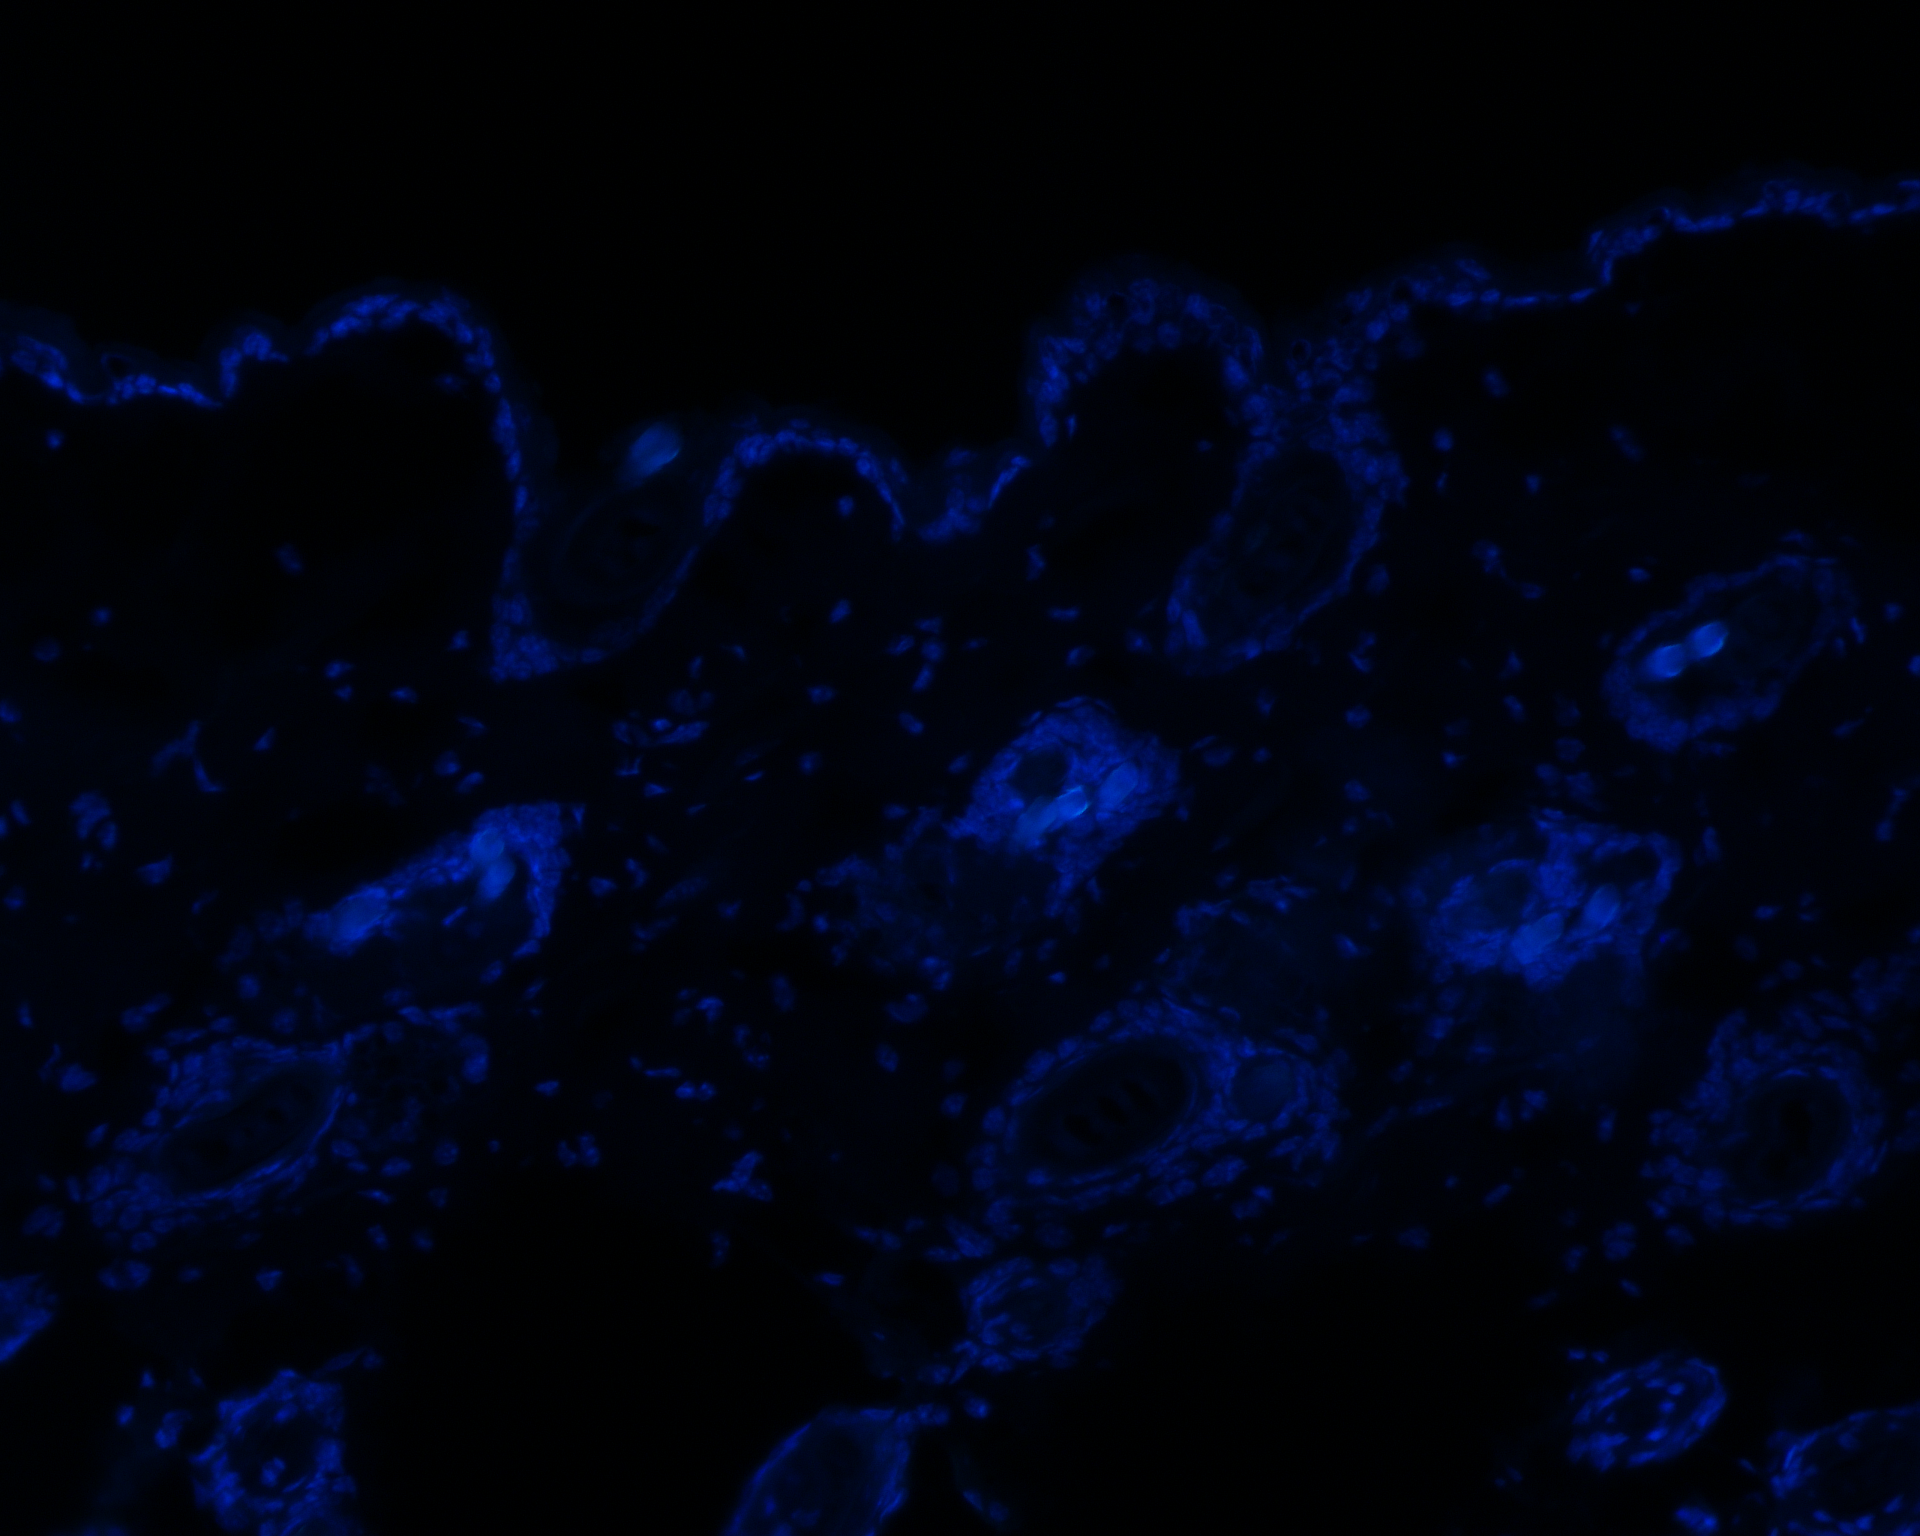
\includegraphics[width=7cm]{./images/1H_Nrf2_No_ADT_1_DAPI}
%\captionsetup{justification=centering}
%\caption{รูปตัวอย่าง dataset}\label{fig:intro}
%\end{figure}
\section{วัตถุประสงค์}
\begin{enumerate}
 	\item เพื่อพัฒนาแบบจำลองสำหรับนับจำนวนนิวเคลียสจากภาพถ่ายเนื้อเยื่อจากการย้อมด้วยสารเรืองแสง
	\item เพื่อพัฒนาเว็บแอปพลิเคชัน ที่สามารถทำการนับจำนวนนิวเคลียสจากภาพถ่ายเนื้อเยื่อจากการย้อมด้วยสารเรืองแสงได้
\end{enumerate}
\section{ขอบเขตของงานวิจัย}
เป้าหมายของงานวิจัยคือต้องการพัฒนาแบบจำลองที่สามารถตรวจจับตำแหน่งของนิวเคลียสและนับจำนวนของนิวเคลียสได้ และพัฒนาเว็บแอปพลิเคชัน ที่สามารถทำการนับจำนวนนิวเคลียสจากภาพถ่ายเนื้อเยื่อจากการย้อมด้วยสารเรืองแสงได้อย่างถูกต้องและมีประสิทธิภาพ เพื่อช่วยลดเวลาในการนับจำนวนนิวเคลียสของนักพยาธิวิทยา และเพื่อเพิ่มความแม่นยำในการนับจำนวนนิวเคลียสให้มีความแม่นยำมากยิ่งขึ้น ดังนั้นขอบเขตของงานวิจัยจึงมีดังนี้
\begin{itemize}
	\item ศึกษาวิธีการตรวจหาตำแหน่งและนับจำนวนนิวเคลียส ด้วยวิธีการประมวลผลภาพ และการเรียนรู้เชิงลึก เพื่อนำไปสู่การพัฒนาแบบจำลอง
    \item เพื่อพัฒนาแบบจำลองที่สามารถตรวจหาตำแหน่งและนับจำนวนนิวเคลียสในภาพถ่ายเนื้อเยื่อจากการย้อมด้วยสารเรืองแสง
    \item เลือกวิธีการที่ดีที่สุดที่ได้จากการพัฒนาแบบจำลองทั้งหมด เพื่อนำมาใช้กับเว็บแอปพลิเคชัน
	\item พัฒนาเว็บแอปพลิเคชัน ที่สามารถนับจำนวนนิวเคลียสจากภาพถ่ายเนื้อเยื่อจากการย้อมด้วยสารเรืองแสงได้
\end{itemize}
\section{ประโยชน์ที่คาดว่าจะได้รับ}
จากการสร้างเว็บแอปพลิเคชันสำหรับการตรวจนับจำนวนนิวเคลียสจากภาพถ่ายเนื้อเยื่อจากการย้อมด้วยสารเรืองแสง จะช่วยลดเวลาในการนับจำนวนนิวเคลียส เพิ่มความถูกต้องและความแม่นยำในการนับจำนวนนิวเคลียสสำหรับนักพยาธิวิทยาที่ทำเกี่ยวกับภาพถ่ายเนื้อเยื่อจากการย้อมด้วยสารเรืองแสงและเพิ่มประสิทธิภาพในการแปลผลจากภาพถ่ายเนื้อเยื่อจากการย้อมด้วยสารเรืองแสงได้มากขึ้น 
\section{ตารางการดำเนินงาน}
\textbf{ผลการดำเนินงานในภาคการศึกษาที่ 1} ทำการศึกษาข้อมูลและกระบวนการที่เกี่ยวกับอัลกอริทึมในการนับจำนวนนิวเคลียสจากภาพถ่ายเนื้อเยื่อจากการย้อมด้วยสารเรืองแสง และจัดทำรายงานประจําภาคการศึกษาที่ 1 ดังรูปภาพที่ \ref{fig:g1}

\textbf{ผลการดำเนินงานในภาคการศึกษาที่ 2} เว็บแอปพลิเคชันสำหรับการใช้งานอัลกอริทึมในการนับจำนวนนิวเคลียสจากภาพถ่ายเนื้อเยื่อจากการย้อมด้วยสารเรืองแสง และรายงานประจำภาคการศึกษาที่ 2 ดังรูปภาพที่ \ref{fig:g2}
\begin{figure}[!h] 
\centering
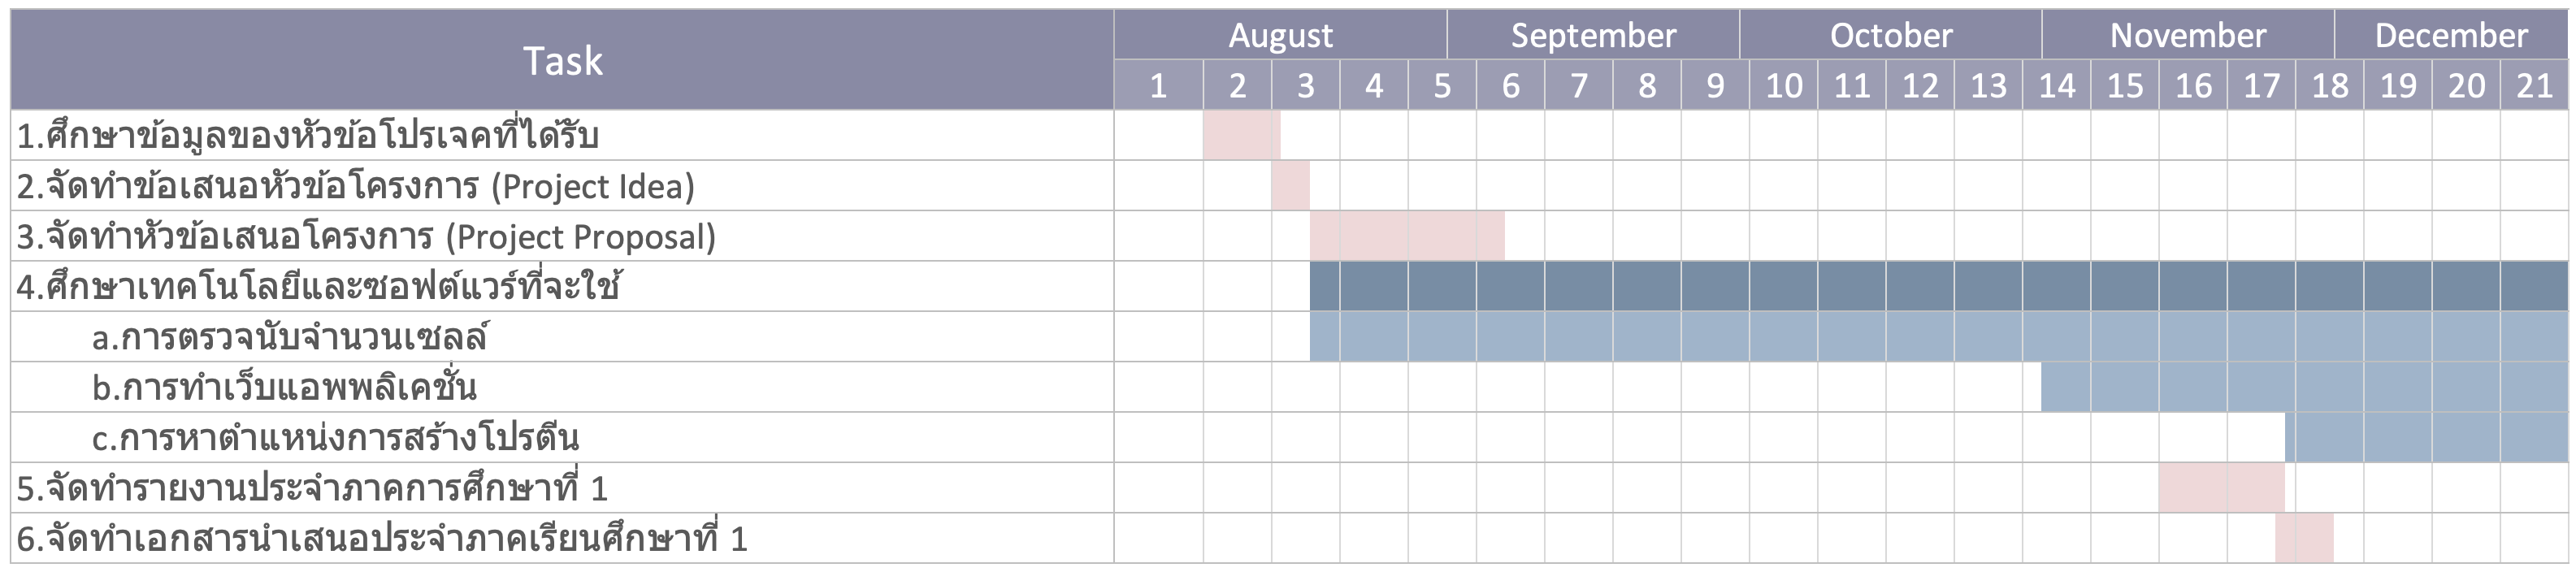
\includegraphics[width=0.9\textwidth]{images/gant1.png}
\caption{ตารางการดำเนินงานในภาคการศึกษาที่ 1}\label{fig:g1}
\end{figure}
% \pagebreak
\begin{figure}[!h]
% \vspace{-7.5in}
\centering
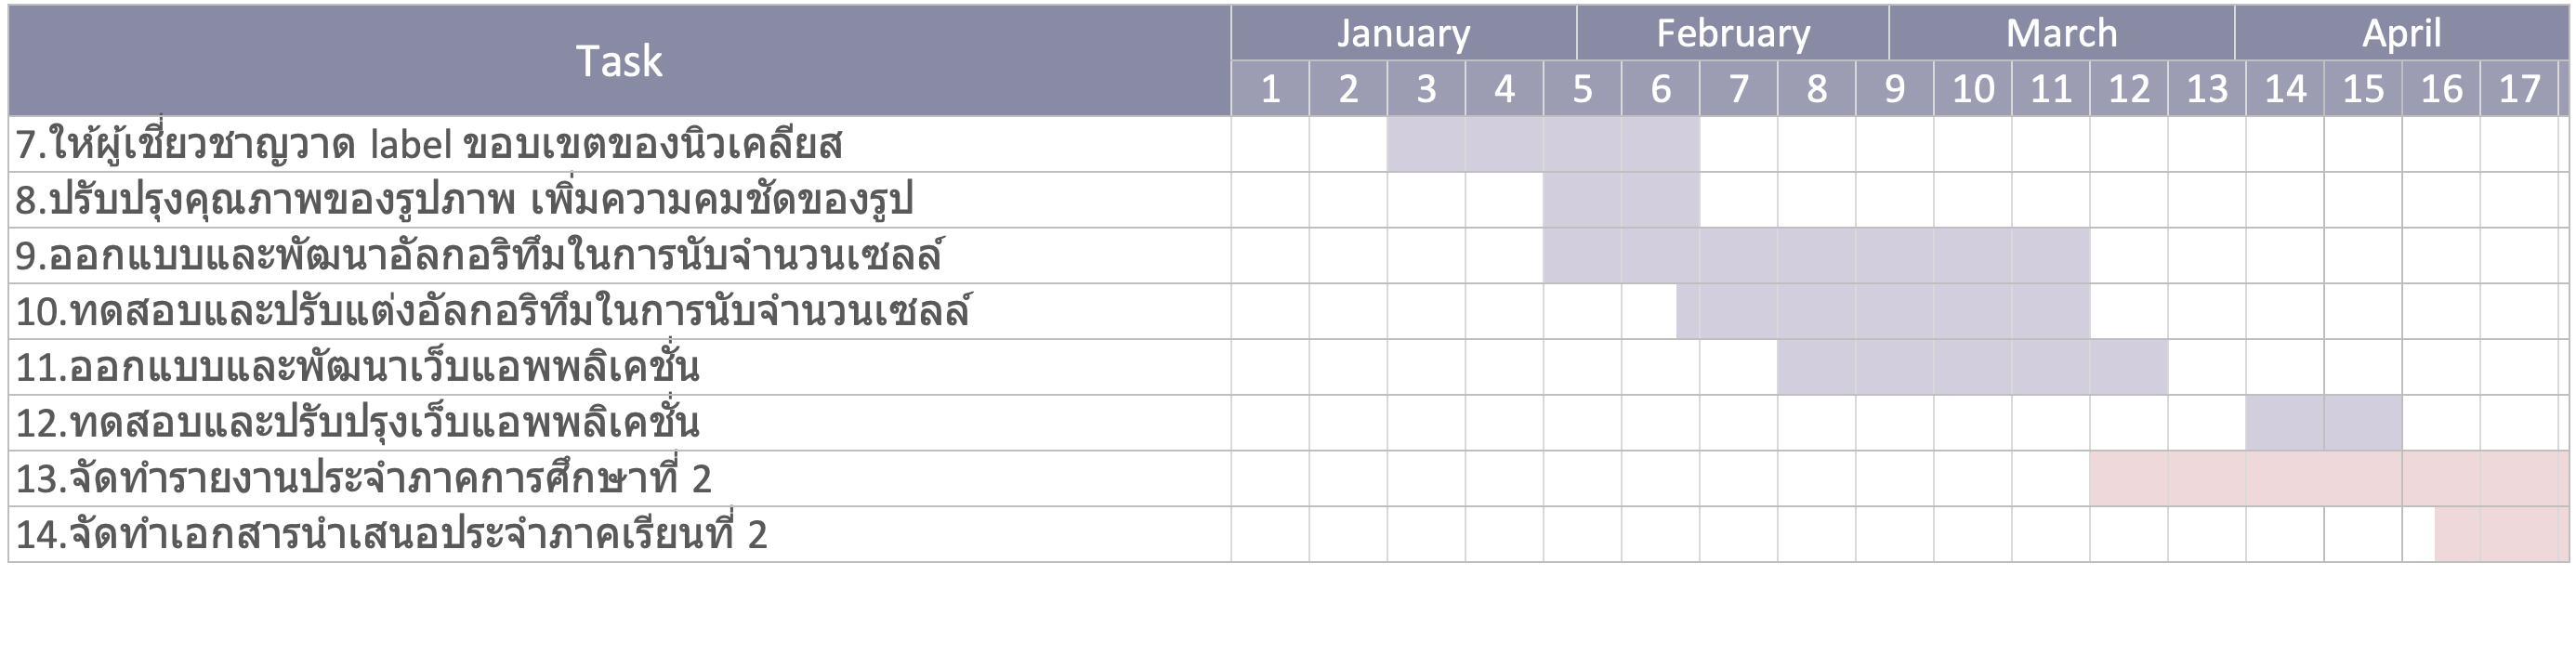
\includegraphics[width=0.9\textwidth]{images/gaint2.png}
\caption{ตารางการดำเนินงานในภาคการศึกษาที่ 2}\label{fig:g2}
\end{figure}
%%%%%%%%%%%%%%%%%%%%%%%%%%%%%%%%%%%%%%%%%%%%%%%%%%%%%%%%%%%%
%%%%%%%%%%%%%%  Literature Review %%%%%%%%%%%%%%%%%%%%%%%%%%
%%%%%%%%%%%%%%%%%%%%%%%%%%%%%%%%%%%%%%%%%%%%%%%%%%%%%%%%%%%%
\chapter{ทฤษฎีความรู้และงานที่เกี่ยวข้อง}
ในบทนี้จะกล่าวถึงรายละเอียดทฤษฎีและงานวิจัยที่เกี่ยวข้องกับการนำการประมวลผลภาพ (Image Processing) และการเรียนรู้เชิงลึก (Deep Learning) มาใช้ในการวิเคราะห์ภาพถ่ายทางพยาธิวิทยา โดยจะกล่าวถึงหลักการ ทฤษฎีที่เกี่ยวข้องที่ใช้ในการทํางานและการศึกษาเพื่อบรรลุวัตถุประสงค์ การอธิบายภาษาทางคอมพิวเตอร์ที่ได้กล่าวถึงและใช้งานในการแก้ไขปัญหา และสุดท้ายคืองานวิจัยที่เกี่ยวข้องกับงานวิจัยนี้ 

\section{ทฤษฎีที่เกี่ยวข้อง}
\subsection{ด้านพยาธิวิทยา}
\subsubsection{อิมมูโนฟลูออเรสเซนซ์ (Immunofluorescence)}
อิมมูโนฟลูออเรสเซนซ์เป็นเทคนิคการวินิจฉัยโดยยึดหลักการจับแอนติเจนและแอนติบอดี การตรวจหาจากฟลูออเรสเซนซ์ ใช้กันอย่างแพร่หลายเพื่อศึกษาตำแหน่งของโปรตีน และสถานะการทำงานของโปรตีนเป้าหมายในนิวเคลียสหรือเนื้อเยื่อ เทคนิคนี้มีความไวและความจำเพาะต่อแอนติเจนจำเพาะสูง โดยแอนติบอดีปฐมภูมิจะจับกับโปรตีนที่สนใจ และแอนติบอดีทุติยภูมิจะจับกับแอนติบอดีปฐมภูมิอีกทีหนึ่ง ซึ่งแอนติบอดีปฐมภูมิจะทำหน้าที่จับกับสารเรืองแสงประเภทต่าง ๆ \cite{12} 
\subsubsection{สารเรืองแสง (Fluorochromes)}
สารเรืองแสง คือ สีย้อมที่มีคุณสมบัติเปล่งแสงได้ สีย้อมนี้มีคุณสมบัติที่จะเข้าทำปฏิกิริยากับนิวเคลียสหรือองค์ประกอบย่อยของนิวเคลียสอย่างจำเพาะ ตัวอย่างเช่น 4',6-diamidino-2-phenylindole (DAPI) จะทำปฏิกิริยากับกรดนิวคลิอิก (Nucleic Acids) โดยจับกับบริเวณ A-T base pair ของ DNA จึงเป็นที่นิยมใช้ในการบ่งบอกตำแหน่งของนิวเคลียส DAPI จะให้สีน้ำเงินเมื่อถูกกระตุ้น นักพยาธิวิทยาสามารถใช้สีย้อมที่หลากหลายโดยมีความจำเพาะต่อส่วนต่าง ๆ ของนิวเคลียสในการบ่งชี้โครงสร้างของนิวเคลียสหลาย ๆ โครงสร้างพร้อมกัน ในการทดลองหลากสีพร้อมกัน ด้วยคุณสมบัติสเปกตรัมของ DAPI ที่เป็นสีน้ำเงินทําให้เหมาะสําหรับใช้ร่วมกับสีเขียว (เช่น Invitrogen Alexa Fluor 488, FITC, GFP) และสีแดง (เช่น Invitrogen Alexa Fluor 594, Rhodamine, Invitrogen Texas Red, mCherry, mKate-2) โดยทั่วไป DAPI จะใช้ย้อมสีนิวเคลียสเพื่อดูตำแหน่งของนิวเคลียสในเซลล์  ซึ่งจะบ่งบอกรูปลักษณะของนิวเคลียส (Nucleus morphology) และจำนวนนิวเคลียส (Nucleus number) ได้
\cite{13}
\subsubsection{ภาพถ่ายเนื้อเยื่อจากการย้อมด้วยสารเรืองแสง (Immunofluorescence Tissue)}
ภาพถ่ายเนื้อเยื่อจากการย้อมด้วยสารเรืองแสง คือภาพถ่ายที่ได้มาจากกระบวนการอิมมูโนฟลูออเรสเซนซ์ และทำการย้อมสีด้วยสารเรืองแสง ซึ่งสามารถบอกตําแหน่งของนิวเคลียสในตัวอย่างเนื้อเยื่อโดยการใช้สีย้อม DAPI ซึ่งจากภาพถ่ายเนื้อเยื่อจากการย้อมด้วยสารเรืองแสงนั้นจะพบว่ามีจำนวนนิวเคลียสรวมตัวอยู่มาก ดังที่แสดงในรูปที่~\ref{fig:Immunofluorescence tissue cell} \cite{14} ซึ่งจะประกอบด้วยสองส่วน คือ ส่วนของเซลล์เดียวที่ลอยแยกกันเดี่ยว ๆ ดังบริเวณที่ลูกศรสีแดงชี้อยู่ อีกส่วนคือเนื้อเยื่อ ซึ่งเป็นปัญหาที่คณะผู้วิจัยสนใจที่จะแก้ไข ดังบริเวณกรอบสีเขียว
\begin{figure}[!h]\centering
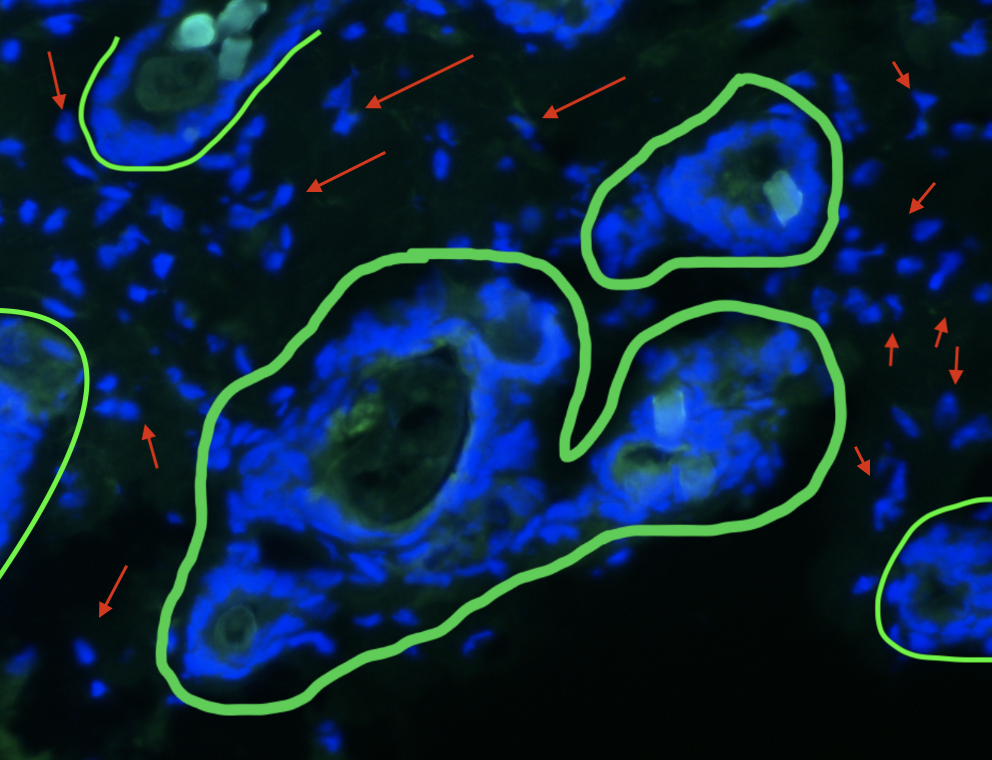
\includegraphics[width=6cm]{images/dataset_test.png}
\caption{ภาพขยายของนิวเคลียสจากภาพถ่ายเนื้อเยื่อจากการย้อมด้วยสารเรืองแสง}\label{fig:Immunofluorescence tissue cell}
\end{figure}
%\subsection{Protein Expression}
%เป็นเทคนิคหนึ่งที่เป็นทางเลือกให้กับนักพันธุวิศวกรรม ที่ต้องการจะผลิตโปรตีนที่ต้องการศึกษาในเวกเตอร์ที่ต้องการ โดยอาศัยเทคนิคทางพันธุวิศวกรรม โดยปกติแล้วในสิ่งมีชีวิตทั่ว ๆ ไปมีการผลิตโปรตีนในนิวเคลียสอยู่แล้ว ซึ่งโปรตีนแต่ละตัวจะถูกผลิตโปรตีนออกมาแตกต่างกัน โปรตีนจะถูกสังเคราะห์และควบคุมโดยขึ้นอยู่กับความต้องการในการทำงานของนิวเคลียสนั้น ๆ โดยโปรตีนจะถูกเก็บไว้ใน DNA และทำการถอดรหัสโดยกระบวนการถอดรหัส (Transcription) เพื่อผลิต messenger RNA (mRNA) โดย mRNA จะถูกเปลี่ยนเป็นโปรตีน\cite{personfff}
\subsection{ด้านคอมพิวเตอร์}
\subsubsection{การประมวลผลภาพ (Image Processing)}
 เป็นวิธีการดำเนินการประมวลผล ปรับปรุง และวิเคราะห์รูปภาพที่อยู่ในรูปแบบดิจิทัลโดยการใช้คอมพิวเตอร์ เพื่อให้ได้มาซึ่งรูปภาพที่มีลักษณะที่ต้องการ ทั้งในเชิงคุณภาพและปริมาณ \cite{15} สามารถนำข้อมูลที่ได้จากรูปภาพไปใช้ประโยชน์ได้ต่อไป ในปัจจุบันการประมวลผลภาพถูกนำมาใช้งานอย่างกว้างขวางในด้านงานวิจัยทางการแพทย์ ซึ่งจะช่วยทำให้สามารถวางแผนการรักษาได้อย่างมีประสิทธิภาพและเพิ่มความถูกต้องแม่นยำในการรักษาให้มากยิ่งขึ้น
\begin{itemize}
% \setlength{\itemindent}{.3in}
\item \textbf{RGB to Grayscale} คือการแปลงภาพสี RGB ให้เป็นภาพ Grayscale ที่มีระดับสี 256 แบบ จาก 0 (ดำ) ถึง 255 (ขาว) ซึ่งสามารถทำได้หลายวิธี เช่นการใช้สมการในการหาค่าเฉลี่ยของ 3 ค่าสีบน RGB \cite{16} หรือวิธีการคูณค่าคงที่กับแต่ละค่าสีของ RGB \cite{17} ดังสมการ \ref{Eq:gray}
\begin{equation}
	Grayscale = (w_{1}*R)+(w_{2}*G)+(w_{3}*B) \label{Eq:gray}
\end{equation}
\hspace*{5mm}
\begin{tabular}{l@{ }l@{ }l@{ }l}
 เมื่อ    & $1 = w_{1}+w_{2}+w_{3}$  และ & $0 < w_{1},$ $w_{2},$ $w_{3}$ \\
        % & $x =$ พิกัดในแนวนอน และ & $y =$ พิกัดในแนวตั้ง\\
        & $Grayscale =$ รูปผลลัพธ์ในช่วงของสีเทา\\
        & $R =$ ช่วงสีแดง & $G =$ ช่วงสีเขียว & และ $B =$ ช่วงสีน้ำเงิน\\
        & $w_{1} =$ น้ำหนักของสีแดง & $w_{2} =$ น้ำหนักของสีเขียว & และ $w_{3} =$ น้ำหนักของสีน้ำเงิน
\end{tabular}

\item\textbf{Histogram Equalization (HE)}
เป็นกระบวนการปรับปรุงค่า Contrast ในรูปภาพ โดยจะทำการยืดค่า Histogram ออกให้กระจายเท่า ๆ กันในแต่ละช่วง ดังนั้นค่าความเข้มแสง (Intensity) จึงกระจายเท่า ๆ กันทั้งช่วงของ Histogram ดังรูปที่ \ref{fig:opencv_he} ซึ่งการจะคำนวนค่า Equalization สามารถหาได้จากการคำนวนค่า Cumulative Distribution Function (CDF) เขียนได้ดังสมการ \ref{Eq:HE1}
\begin{equation}
    H'(i) = \sum_{0\leq j<i} H(i) \label{Eq:HE1}
\end{equation}
\hspace*{5mm}
\begin{tabular}{l@{ }l@{ }l}
 เมื่อ    & $H(i) =$ Histogram \\
        & $H'(i) =$ Cumulative Histogram \\
        & $i =$ Max intensity (default is 255)
\end{tabular}

จากนั้นทำการ Normalize $H'(i)$ ให้อยู่ในช่วงค่าความเข้มแสง (Intensity) สูงที่สุดของรูปภาพ \cite{HE} เขียนได้ดังสมการ \ref{Eq:HE2}
\begin{equation}
    Equalized = H'(i)(src) \label{Eq:HE2}
\end{equation}
\begin{tabular}{l@{ }l@{ }l}
  เมื่อ   & $src_{(x,y)} =$ Input Image \\ & $Equalized =$ ผลลัพธ์ของ HE
\end{tabular}
\begin{figure}[!h]\centering
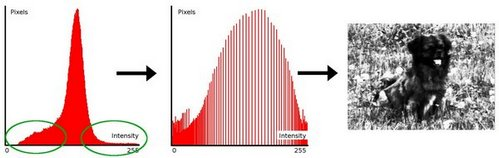
\includegraphics[width=8cm]{images/he_opencv}
\captionsetup{justification=centering}
\caption[ตัวอย่างการกระจายค่า Histogram Equalization]{ตัวอย่างการกระจายค่า Histogram Equalization \cite{img_histogram}}\label{fig:opencv_he}
\end{figure}

\item\textbf{Contrast Limited Adaptive Histogram Equalization (CLAHE)}
เป็นกระบวนการหนึ่งในกลุ่มของ Adaptive Histogram Equalization (AHE) ซึ่งจะให้ความสนใจในการขยายสัญญาณที่มากเกินไปของ Contrast ช่วยปรับปรุงค่า Contrast ของรูปให้ดียิ่งขึ้น กระบวนการ CLAHE จะไม่ทำงานทั้งรูป แต่จะทำงานบนช่วงเล็ก ๆ ของรูปเรียกว่า Tile โดยชิ้นส่วน Tile อื่น ๆ จะถูกนำมารวมด้วย Bilinear Interpolation เพื่อลบ Artificial Boundaries \cite{23} โดยค่า Histogram ที่มีระดับสูงกว่าค่าเฉลี่ยของพิกเซลจะถูกนำมากระจายให้ทุกพิกเซลในภาพ ดังรูปที่~\ref{fig:hisss}. \cite{24}
\begin{figure}[!h]\centering
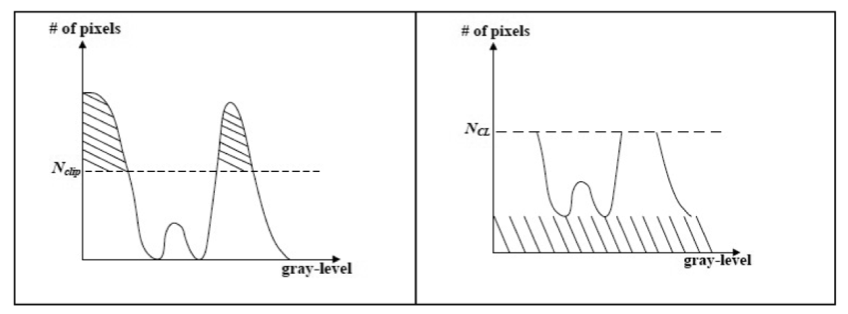
\includegraphics[width=8cm]{images/Screenshot 2022-11-16 at 10.51.45 PM}
\captionsetup{justification=centering}
\caption[หลักการกระจายค่า Histogram ของ CLAHE]{หลักการกระจายค่า Histogram ของ CLAHE \cite{image_CLAHE}} \label{fig:hisss}
\end{figure}

\item\textbf{Thresholding}
กระบวนการแปลงภาพเป็นภาพ Binary หรือภาพที่มีเฉพาะสีดำคือค่า Intensity เป็น 0 และสีขาวคือค่า Intensity เป็น 1 เพื่อแยกวัตถุออกจากพื้นหลังอย่างชัดเจน โดยพิจารณาจากค่า Intensity ของแต่ละ Pixel เปรียบเทียบกับ Threshold Value ถ้าค่า Intensity มากกว่า Threshold Value จะแปลงค่า Intensity เป็น 1 หรือสีขาว และถ้าค่า Intensity น้อยกว่า Threshold Value จะแปลงค่า Intensity เป็น 0 หรือสีดำ ซึ่งโดยทั่วไปจะทำกับภาพ Grayscale มีระดับสีหรือค่า Intensity 0 (ดำ) ถึง 255 (ขาว) \cite{20} เนื่องจากภาพจะมีรูปแบบเก็บข้อมูลแบบ 2 ส่วน คือ Foreground(วัตถุหรือสิ่งที่สนใจ) และ Background(พื้นหลังของภาพ) ซึ่งจะสามารถจำแนกวัตถุง่ายกว่าภาพสี \cite{21}

% \item\textbf{K-means}
% เป็นกระบวนการอย่างหนึ่งในกลุ่มของ Unsupervised Learning โดยมีเป้าหมายในการแบ่งกลุ่มข้อมูล (Cluster) ที่มีลักษณะใกล้เคียงกัน โดยเราจะทำการกำหนดค่า $K$ แทนด้วยจำนวนกลุ่มที่แบ่งโดยการเฉลี่ย (means) มีทั้งหมด 4 ขั้นตอนดังนี้
% \hspace{5mm}
% \begin{enumerate}
% \item กำหนดจำนวนกลุ่มขึ้นมาก่อน เช่น $K=2$ (กำหนดเป็น $C1$ และ $C2$) และสุ่มตำแหน่งแกน $x,y$ ให้กับ $C1$ และ $C2$ ซึ่งจะได้ $C1_{(x1,y1)}$ และ $C2_{(x2,y2)}$ จุด $C$ แต่ละจุดนั้นเรียกว่าจุด Centroid
% \item ดูตำแหน่งของสมาชิกแต่ละสมาชิกว่าอยู่ใกล้ใครมากกว่ากันก็ให้คนนั้นเป็นสมาชิกของ $C$ นั้น จากตรงนี้เราจะรู้แล้วว่าสมาชิกแต่ละคนอยู่ในกลุ่มใดระหว่าง $C1$ และ $C2$
% \item ปรับ $x,y$ ของ $C1$ และ $C2$ ใหม่ให้อยู่ตรงกลางของกลุ่ม
% \item วนซ้ำ ข้อ 2 และข้อ 3 อีกครั้งจนกว่า $C1$ และ $C2$ ตำแหน่งไม่เปลี่ยน \cite{Kmeans}
% \end{enumerate}
% ซึ่งเราสามารถนำมาประยุกต์ใช้กับการประมวลผลภาพได้ โดยจะต้องแปลงรูปภาพให้อยู่ในรูปแบบ Array 1 มิติก่อนจะนำไปใช้งาน \cite{KmeanOpencv}

\item\textbf {Gaussian Blur}
กระบวนการเบลอภาพด้วยการใช้ค่าเฉลี่ยแบบถ่วงน้ำหนัก ที่ใช้ฟังก์ชันเกาส์เซียนในการคำนวณ แปลงค่าแต่ละพิกเซลเพื่อลบสัญญาณรบกวนในรูปภาพทำให้ความคมชัดของรูปภาพลดลง ซึ่งภาพจะเบลอน้อย และคงเส้นขอบในภาพได้ โดยใช้สมการฟังก์ชันเกาส์เซียน \cite{18} ดังสมการ \ref{Eq:gss}
\begin{equation}
	G(x) = \frac{1}{\sqrt{2\pi\sigma} } e^{\frac{-x^2}{2\sigma^2}} \label{Eq:gss}
\end{equation}
\hspace*{5mm}
\begin{tabular}{l@{ }l@{ }l}
  เมื่อ   & $G(x) =$ ผลลัพธ์กระบวนการเบลอภาพด้วย Gaussian Blur \\
        & $x =$ ระยะทางจากจุดกำเนิดในแนวนอน  \\
        & $\sigma =$ ค่าเบี่ยงเบนมาตรฐานของการแจกแจงแบบเกาส์เซียน
\end{tabular}

% \item\textbf{Canny Edge Detection}
% เป็นวิธีหนึ่งใน Edge detection ในกลุ่มของ Gradient method ที่มุ่งเน้นให้ขอบของวัตถุเด่นชัดขึ้น โดยเปรียบเทียบจากการเปลี่ยนแปลงของ Intensity อย่างรวดเร็วในตําแหน่งที่ใกล้เคียงกับจุดดังกล่าว โดยงานวิจัยของเราได้เลือกใช้ Gradient method ซึ่งจะหาจุดต่ำสุดและจุดสูงสุดของอนุพันธ์อันดับหนึ่งของรูปภาพ \cite{edge_detection} แบ่งได้เป็น 4 ขั้นตอนดังนี้
% \hspace{5mm}
% \begin{enumerate}
%     \item Noise Reduction โดยใช้วิธี Gaussian Blur ที่กล่าวไปก่อนหน้า เพื่อทำการกำจัดสัญญาณรบกวนที่อยู่ในรูปภาพก่อน
%     \item Finding Intensity Gradient of the Image รูปภาพที่ผ่านการลดสัญญาณรบกวนจะถูกนำมาผ่าน Sobel filter ซึ่งใช้การคำนวนอนุพันธ์อันดับหนึ่งในทิศทางแนวนอน $G_{x}$ และแนวตั้ง $G_{y}$
%     เขียนได้ดังสมการ \ref{Eq:edge1}
% \begin{equation}
%     \|\nabla I\| = \sqrt{ G_{x}^2 + G_{y}^2} \\
%     \text{ Where: } G_{x} = \frac{\partial I}{\partial x}\text{ and } G_{y} = \frac{\partial I}{\partial y}\label{Eq:edge1}
% \end{equation}
% \hspace{5mm}
% \begin{tabular}{l@{ }l@{ }l}
%    เมื่อ  & $\|\nabla I\| =$ Gradient magnitude\\
%         & $I =$ Input Image \\
% \end{tabular} \\
% ส่วนการจะหาทิศทางขององศาการเอียงของขอบวัตถุ \cite{opencv} สามารถหาได้จากสมการ \ref{Eq:edge2}
% \begin{equation}
%     \theta = {\tan}^{-1}(\frac{G_{y}}{G_{x}}) \label{Eq:edge2}
% \end{equation}
%     \item Non-maximum Suppression หลังจากได้ค่า Gradient magnitude และ ทิศทางของขอบวัตถุแล้ว จะทำการตรวจสอบทั้งรูปภาพเพื่อกำจัดพิกเซลที่ไม่ได้เป็นส่วนประกอบของขอบวัตถุ ดังรูปที่ \ref{fig:nms}
% \begin{figure}[!h]\centering
% 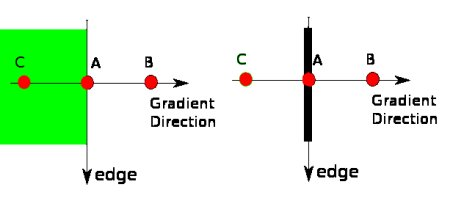
\includegraphics[width=7cm]{images/nms.jpg}
% \captionsetup{justification=centering}
% \caption[ตัวอย่างการทำ Non-maximum Suppression]{ตัวอย่างการทำ Non-maximum Suppression \cite{img_canny}}\label{fig:nms}
% \end{figure}
% โดยจุด A จะเป็นจุดที่อยู่บนขอบวัตถุ (ในทิศทางแนวตั้ง) และจุด B, และ C จะอยู่บนทิศทางของขอบวัตถุ ดังนั้นจุด A จะถูกเลือกให้เป็นขอบของวัตถุ และกำจัดจุด B, และ C ซึ่งจะได้ผลลัพธ์เป็น Binary ที่มีขอบวัตถุแบบบางๆ
% \item Hysteresis Thresholding เป็นขั้นตอนที่จะกำหนดค่าว่าขอบวัตถุไหนคือขอบวัตถุจริง โดยจะกำหนดค่า Threshold 2 ค่าเป็นช่วงพิจารณา ประกอบด้วย minVal, และ maxVal โดยขอบวัตถุมีค่าสูงกว่า maxVal หมายความว่า เป็นขอบจริง ส่วนขอบวัตถุที่มีค่าน้อยกว่า minVal หมายความว่า ไม่เป็นขอบวัตถุจริง ดังรูปที่ \ref{fig:hysteresis}
% \begin{figure}[!h]\centering
% 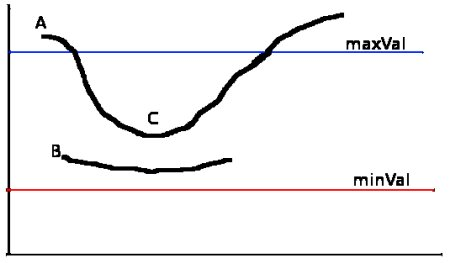
\includegraphics[width=7cm]{images/hysteresis.jpg}
% \captionsetup{justification=centering}
% \caption[ตัวอย่างการทำ Hysteresis Thresholding]{ตัวอย่างการทำ Hysteresis Thresholding \cite{img_canny}}\label{fig:hysteresis}
% \end{figure}
% จะเห็นได้ว่า ขอบวัตถุในช่วง A นั้นอยู่เหนือค่า maxVal ส่งผลให้เป็นขอบวัตถุจริง ต่อมาในช่วง C จะเห็นได้ว่าอยู่ในช่วงพิจารณา ซึ่งค่าของช่วง C เป็นค่าต่อเนื่องมาจากช่วง A ดังนั้นส่งผลให้ช่วง C เป็นขอบวัตถุจริงเช่นกัน ถึงแม้ว่าช่วง B จะอยู่ในช่วงพิจารณาเหมือนกัน แต่ไม่ได้มีค่าต่อเนื่องที่อยู่เหนือค่า maxVal จึงส่งผลให้ไม่เป็นขอบวัตถุจริง
% \end{enumerate}

\item\textbf{Morphological Operation} เทคนิคสำหรับการวิเคราะห์และประมวลผลภาพ โดยการเปลี่ยนแปลงลักษณะของรูปร่างหรือโครงสร้างของภาพ ซึ่งอาศัยโครงสร้างทางเรขาคณิตบนพื้นฐานของทฤษฎีเซต ทฤษฎีตาข่ายโครงสร้างของเครือข่าย และฟังก์ชันแบบสุ่ม การประมวลผลจะเปรียบเทียบพิกเซลในภาพกับพื้นที่ใกล้เคียงโดยการเลือกขนาดและรูปร่างของพื้นที่ใกล้เคียงจะมีตัวดำเนินการหลายแบบ เช่น Dilation การขยายภาพโดยมีสัดส่วนเท่ากันทั้งภาพตัวอย่างในภาพที่~\ref{fig:second} Erosion คือการกร่อนขนาดของบริเวณของของวัตถุตัวอย่างในภาพที่~\ref{fig:third} Skeleton จะเป็นการหาโครงสร้างหลักของวัตถุ Opening การนำข้อมูลภาพ ผ่านการขยายภาพ (Erosion) และตามด้วยการกร่อนภาพ (Dilation) โดยใช้ Template เหมือนกันตัวอย่างในภาพที่~\ref{fig:opening} และ Closing จะทำการกร่อนภาพก่อนแล้วตามด้วยการขยายภาพ โดยใช้ template ชุดเดียวกันตัวอย่างในภาพที่~\ref{fig:closing} \cite{22}

\begin{figure}[h!]
\centering
\begin{subfigure}{0.3\textwidth}
\centering
    
\includegraphics[width=0.5\textwidth]{images/j.png}
    \caption{ภาพต้นฉบับ}
    \label{fig:first}
\end{subfigure}
\hfill
\begin{subfigure}{0.3\textwidth}
\centering
    
\includegraphics[width=0.5\textwidth]{images/dilation.png}
    \caption{ภาพที่ผ่านกระบวนการ Dilation}
    \label{fig:second}
\end{subfigure}
\hfill
\begin{subfigure}{0.3\textwidth}
\centering
    
\includegraphics[width=0.5\textwidth]{images/erosion.png}
    \caption{ภาพที่ผ่านกระบวนการ Erosion}
    \label{fig:third}
\end{subfigure}
\caption[Dilation และ Erosion]{Dilation และ Erosion \cite{2223}
}
\label{fig:figures}
\end{figure}
\begin{figure}[h!]
\centering
\begin{subfigure}{.5\textwidth}
  \centering
  
\includegraphics[width=4cm]{images/opening.png}    \caption{ภาพที่ผ่านกระบวนการ opening}
  \label{fig:opening}
\end{subfigure}%
\begin{subfigure}{.5\textwidth}
  \centering
  
\includegraphics[width=4cm]{images/closing.png}    \caption{ภาพที่ผ่านกระบวนการ Closing}
  \label{fig:closing}
\end{subfigure}
\caption[Opening และ Closing]{Opening และ Closing\cite{2223}}
\label{fig:test_1}
\end{figure}
\pagebreak
\item\textbf{Watershed}
เป็นวิธีหนึ่งในการทำ Image Segmentation โดยมีหลักพื้นฐานมาจากการที่มองว่ารูปภาพ Grayscale สามารถมองเป็นระดับความสูงได้จากค่า Intensity เรียกว่า Topographic surface ดังรูปภาพที่ \ref{fig:wawater1} ดังนั้นวัตถุจะสูงขึ้นมาจากพื้นหลัง ถ้าเราค่อย ๆ เทน้ำลงไปในรูปเรื่อย ๆ ระดับน้ำจะเพิ่มสูงขึ้นเรื่อยๆ จนเหลือเพียงแค่ส่วนยอดที่เหนือพ้นน้ำ ซึ่งจะได้ผลลัพธ์เป็นการแบ่งของวัตถุ ดังรูปภาพที่ \ref{fig:wawater2}
\begin{figure}[h!]
\centering
\begin{subfigure}{.5\textwidth}
  \centering
  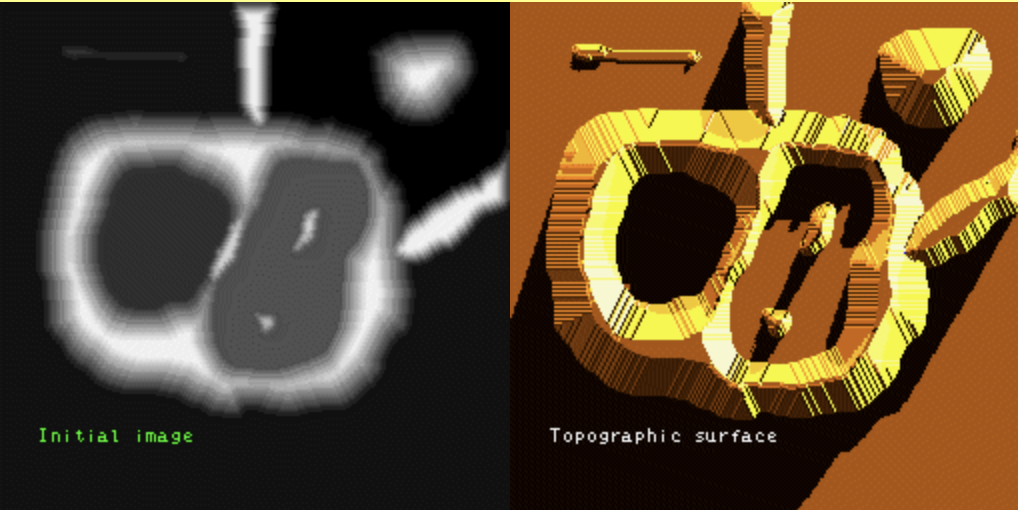
\includegraphics[width=5cm]{images/wt2.png}    \caption{Initial image และ Topographic sueface}
  \label{fig:wawater1}
\end{subfigure}%
\begin{subfigure}{.5\textwidth}
  \centering
  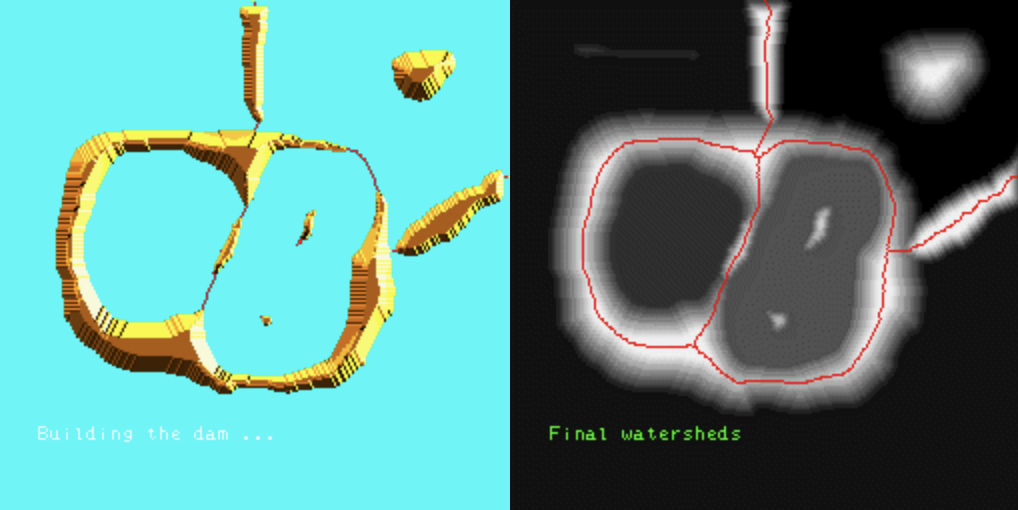
\includegraphics[width=5cm]{images/wt1.png}    \caption{Watersheding และ Final Watershed}
  \label{fig:wawater2}
\end{subfigure}
\caption[Watershed]{Watershed \cite{img_watershed}}
\label{fig:watersherd}
\end{figure}
\end{itemize}

\subsubsection{การเรียนรู้เชิงลึก (Deep Learning)}
การเรียนรู้เชิงลึก คือ การพัฒนาเทคโนโลยีคอมพิวเตอร์ให้สามารถเลียนแบบการทํางานของมนุษย์ ซึ่งการเรียนรู้เชิงลึกจะมีกระบวนการคิดคํานวณคล้ายกับระบบโครงข่ายประสาท (Neurons) ของสมองมนุษย์เรียกว่า โครงข่ายประสาทเทียม (Neural Network: NN) ความสามารถขอการเรียนรู้เชิงลึกสามารถสร้างแบบจําลองและหาคําตอบได้ด้วยการนำโครงข่ายประสาทเทียมหลาย ๆ ชั้นเรียกว่า Hidden Layer มาใช้วิเคราะห์และหาคําตอบ ซึ่งคําว่าการเรียนรู้เชิงลึกก็มาจากการใช้โครงข่ายประสาทเทียมมากกว่า 2 ระดับชั้นขึ้นไปในการสร้างแบบจําลอง ดังนั้นจึงเปรียบได้ว่าจำนวนระดับชั้นของโครงข่ายประสาทเทียมยิ่งถูกใช้จํานวนมากในขั้นตอนการประมวลผล ยิ่งทําให้มีโครงสร้างการเรียนรู้ที่ลึกมากขึ้น ถัดไปจะเป็นการยกตัวอย่างแบบจำลองที่พบในงานวิจัยและมีการนำมาใช้งานกันอย่างแพร่หลาย ได้แก่
\begin{itemize}

\item\textbf{Region-based CNNs (R-CNN)}
เป็นหนึ่งในแนวทางการนำการเรียนรู้เชิงลึกมาใช้กับการตรวจจับวัตถุ โดย RCNN จะทำการแยกรูปภาพออกจากรูป input หลังจากนั้นจะใช้ โครงข่ายประสาทคอนโวลูชัน (Convolutional Neural Network) ในการส่งต่อข้อมูลเพื่อทำการแยกคุณลักษณะต่าง ๆ ต่อไป โดยคุณสมบัติ R-CNN คือต้องการศึกษาการทำนายวัตถุที่ตรวจจับได้ของแต่ละ region โดยกระบวนการทำงานของ R-CNN สามารถแบ่งย่อยได้เป็น 4 ขั้นตอนหลัก ๆ คือ ทำการเลือกขอบเขตที่สนใจออกจากรูป input โดยส่วนใหญ่ขอบเขตที่ได้เลือกนั้นจะมีรูปร่างหรือขนาดที่แตกต่างกัน โดยแต่ละขอบเขตจะทำการระบุตำแหน่งของ class และ ground-truth ไว้ ต่อมาจะนำ pretrained CNN ที่ได้ฝึกไว้มาทำการปรับขนาดของรูปที่ได้ก่อนที่จะทำการแยกคุณลักษณะต่าง ๆ ถัดมาจะมีการนำ support vector machine มาใช้ในการจำแนกวัตถุ และทำการฝึกอบรมแบบจำลอง linear regression เพื่อใช้ในการทำนาย region ตามความเป็นจริง โดยมีโครงสร้างดังที่รูปภาพที่ \ref{fig:แบบจำลอง R-CNN} \cite{rCNN}
\begin{figure}[!h]\centering
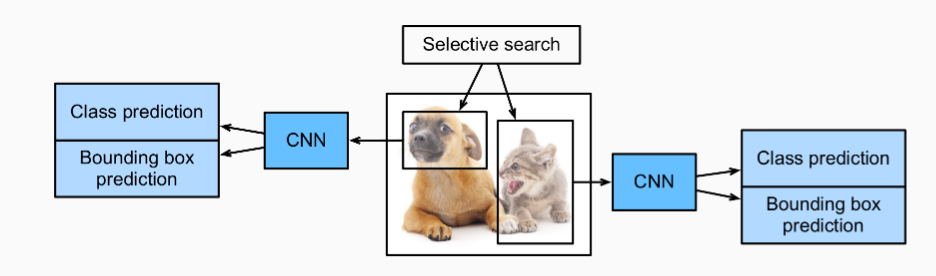
\includegraphics[width=11cm]{images/RCNN model image.png}
\caption[แบบจำลอง R-CNN]{แบบจำลอง R-CNN \cite{img_rcnn}} \label{fig:แบบจำลอง R-CNN}
\end{figure}
\pagebreak
\item\textbf{Mask R-CNN}
Mask R-CNN ปรับปรุงจาก Faster R-CNN ซึ่งพัฒนามาจาก Region-based CNNs โดยการเพิ่มการทํานาย mask ของวัตถุ โดยจะทำงานควบคู่ไปกับ Faster R-CNN ที่จะจดจําขอบเขตของวัตถุ มีโครงสร้างดังรูปภาพที่ \ref{fig:mrcnn} มีพื้นฐานแนวคิดที่เรียบง่าย ยืดหยุ่น และทั่วไป และมีแนวทางตรวจจับวัตถุในภาพได้อย่างมีประสิทธิภาพสูงในการแบ่งแต่ละ mask นอกจากนี้ Mask R-CNN มีลักษณะการเรียนรู้ที่ง่ายและมีประสิทธิภาพ ช่วยลดความยากในงานวิจัยในอนาคต 
โดยสถาปัตยกรรมโครงสร้างของ Mask R-CNN แต่ละขั้นตอนสามารถอธิบายได้ ดังนี้
    \begin{itemize}
        \item ภาพชุดข้อมูลจะถูกส่งผ่านโครงข่ายคอนโวลูชัน
        \item ผลลัพธ์ที่ได้จากการทำโครงข่ายคอนโวลูชันแรกจะถูกส่งผ่านไปยัง Region Proposal network (RPN) ซึ่งจะสร้าง achor box (ตำแหน่งที่สนใจ) ที่แตกต่างกันตามการมีอยู่ของอ็อบเจ็กต์นั้น ๆ ที่จะตรวจจับได้
        \item Anchor box จะถูกส่งไปยัง ROI Align stage (เป็นหนึ่งในฟีเจอร์หลักของ Mask RCNN สำหรับการป้องกันการจัดวางเชิงพื้นที่) ซึ่งจะแปลง ROI ให้เป็นขนาดเดียวกันกับที่จำเป็นสำหรับการประมวลผลเพิ่มเติม
        \item ผลลัพธ์นี้ถูกส่งไปยังเลเยอร์ที่เชื่อมต่อกัน ซึ่งจะสร้างผลลัพธ์ของคลาสของวัตถุในพื้นที่นั้น ๆ และหาตำแหน่งของกล่องของวัตถุ
        \item ผลลัพธ์ของระยะ ROI Align จะถูกส่งไปยัง Conv Nets เพื่อสร้างหน้ากากของพิกเซลของวัตถุนั้น
    \end{itemize}
ซึ่งแบบจำลองนี้จะมีพารามิเตอร์ทั้งหมดประมาณ 64 ล้านพารามิเตอร์ \cite{model_maskpara} มีโครงสร้างแบบจำลองดังตารางที่ \ref{tbl:maskrcnnarchitech} 
โดยคณะผู้วิจัยได้เลือกวิธีการ Mask R-CNN ในการทดลองแทน R-CNN เนื่องจาก R-CNN ใช้ Support Vector Machine ในการแยกประเภทและต้องรู้จำพื้นที่ย่อยทุกอันในลักษณะหมือนเริ่มจากศูนย์ทุกครั้ง นั่นคือถ้า region ถูกเสนอมา 2,000 ส่วน ก็ต้องทำเสมือนการรู้จำภาพที่เป็นอิสระจากกัน 2,000 ครั้ง เท่ากับต้องคำนวณ CNN ใหม่ 2,000 รอบ R-CNN จึงใช้ Computational Resource อย่างมาก \cite{markrcnn}

\begin{figure}[!h]
    \centering
    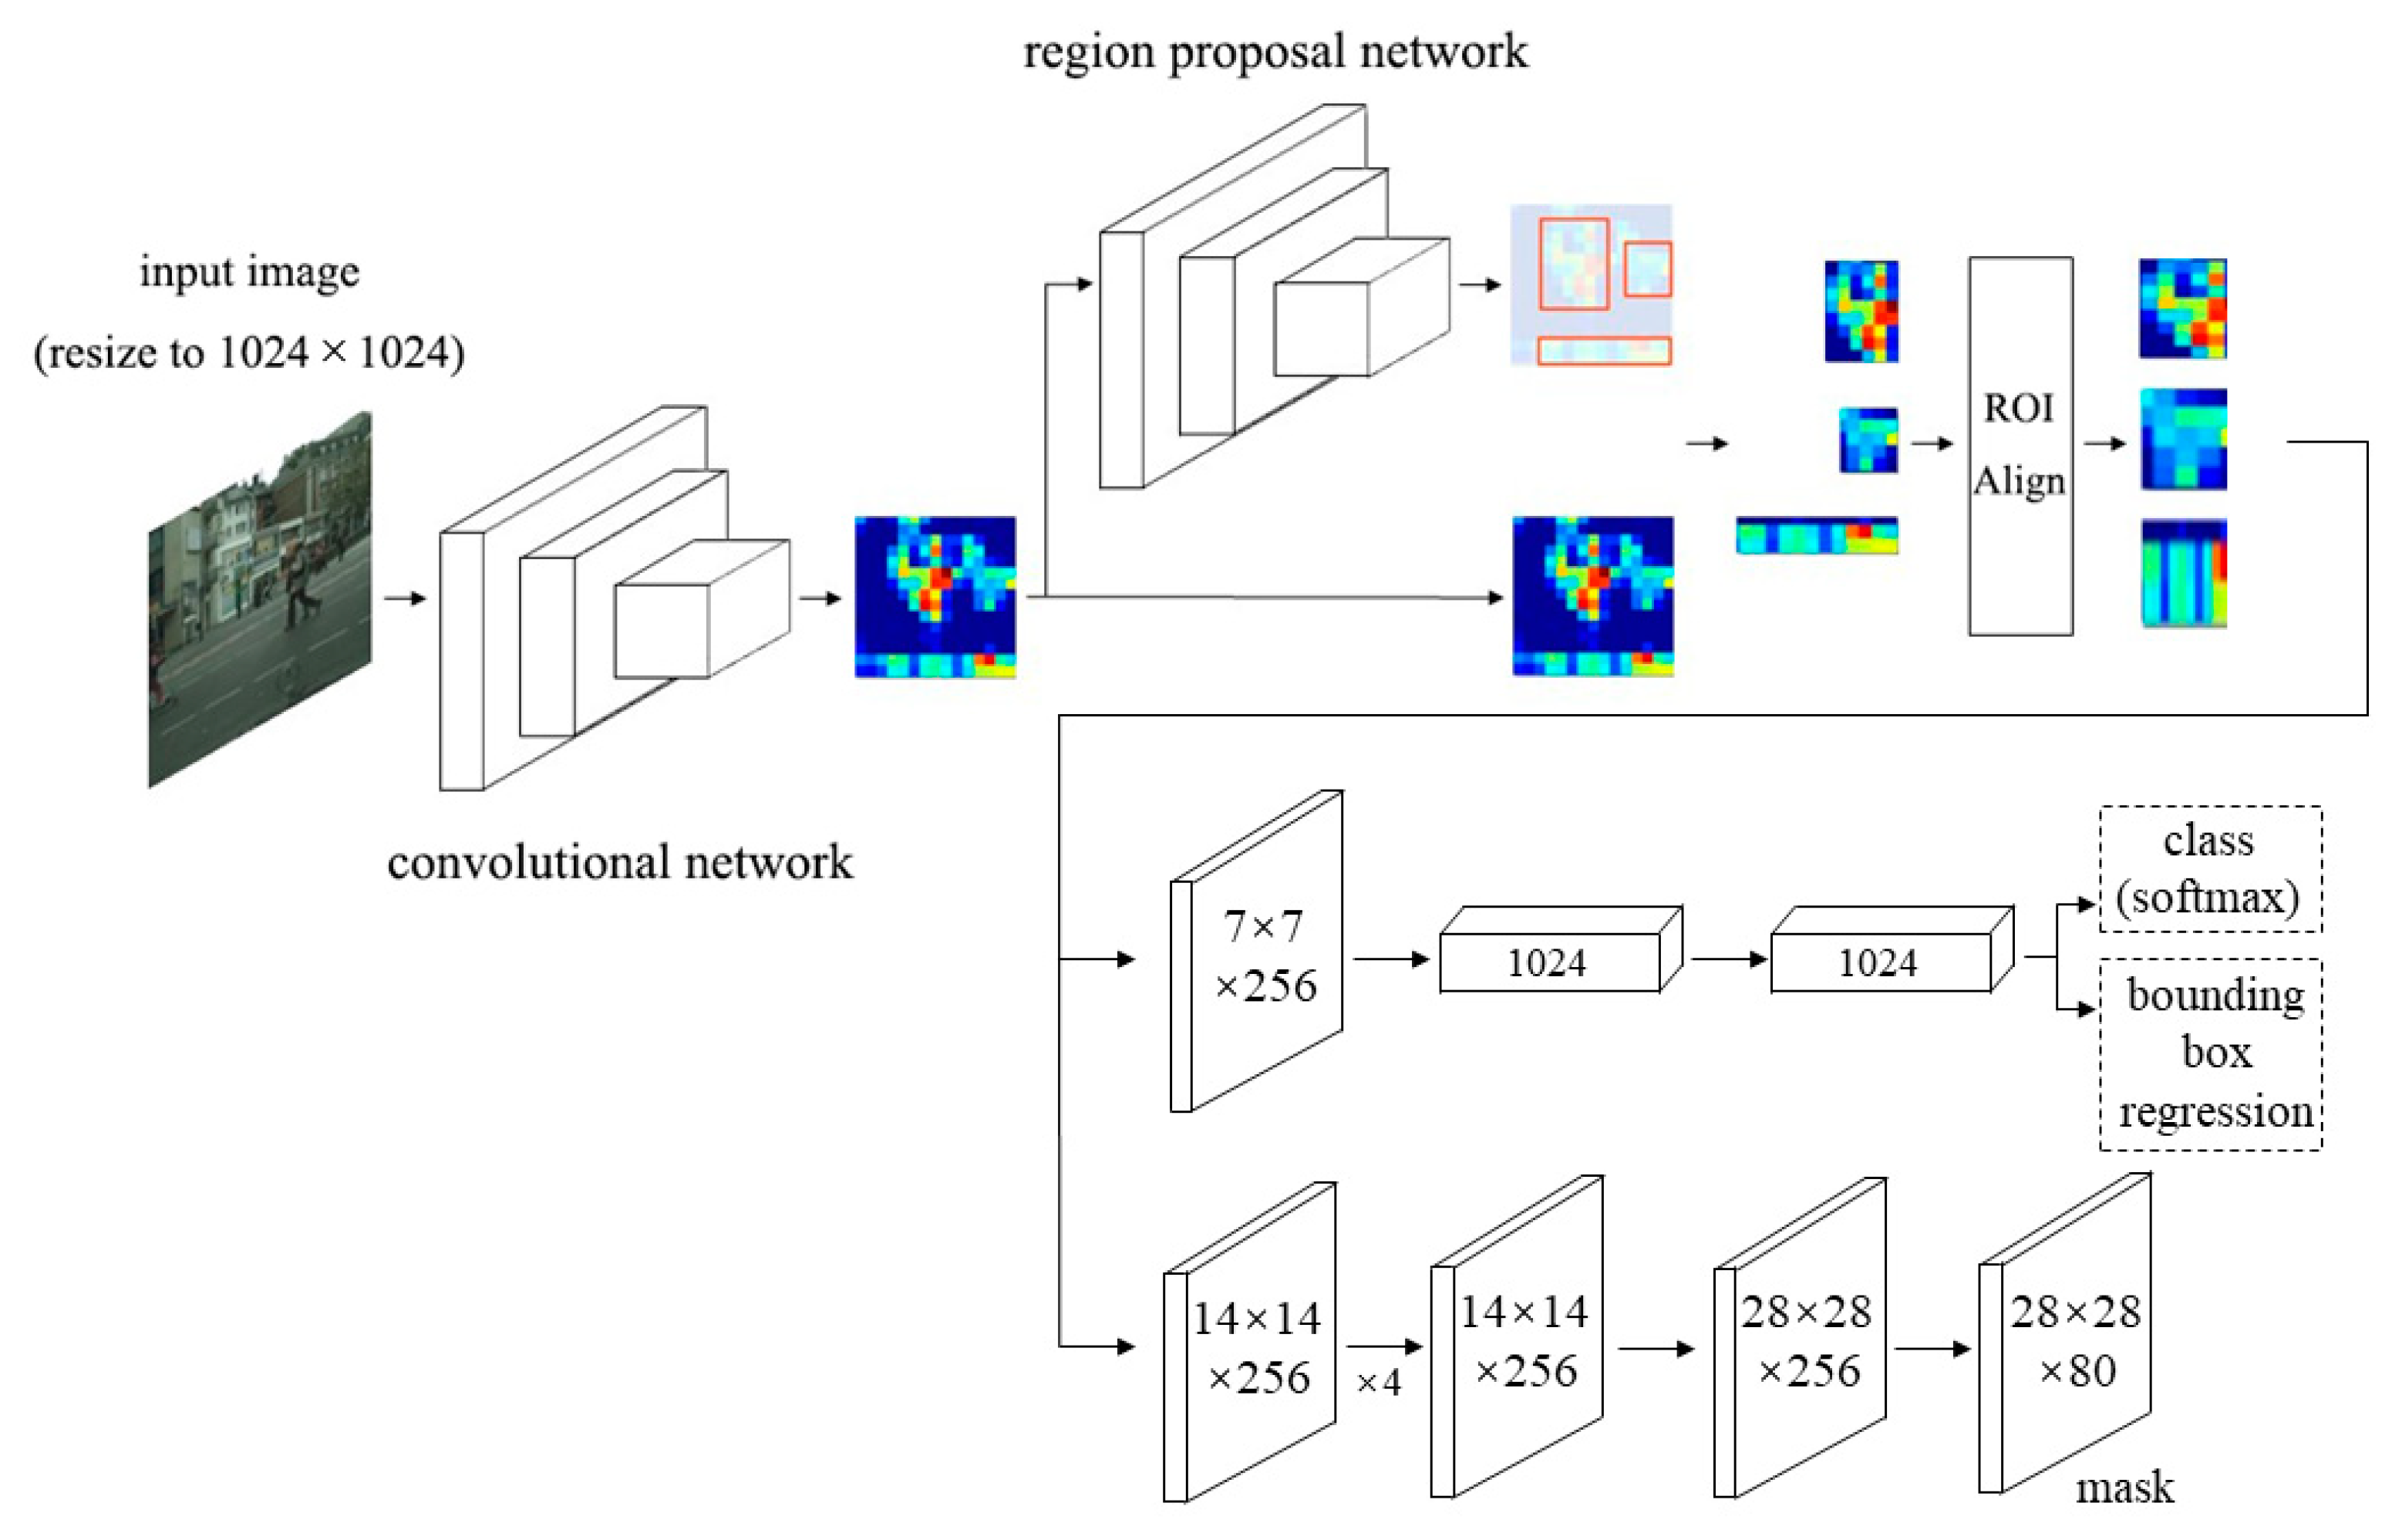
\includegraphics[width=8cm]{images/sensors-20-01010-g003.png}
    \caption[แบบจำลอง Mask R-CNN]{แบบจำลอง Mask R-CNN \cite{img_maskrcnn}}
    \label{fig:mrcnn}
\end{figure}

\begin{table}[!h]
\centering
\caption{Mask R-CNN architecture}\label{tbl:maskrcnnarchitech}
\begin{tabular}{p{0.3\textwidth}>{\raggedright\arraybackslash}p{0.6\textwidth}}
\toprule
layers  & Description  \\ \midrule
\textbf{Input Layers:} &  \\
\quad Input layer: & shape = (batch\_size, 512, 512, 3) \\ 
\textbf{Backbone Layers: } & \\
\quad Convolutional Block1 & 7x7, 64, stride 2, padding same, activation ReLU \\
\quad MaxPooling & 3x3, stride 2 \\
\quad Residual Convolutional Block2 & 3x3, 64 filters, 3 blocks \\
\quad Residual Convolutional Block3 & 4x4, 128 filters, 4 blocks \\
\quad Residual Convolutional Block4 & 6x6, 256 filters, 23 blocks \\
\quad Residual Convolutional Block5 & 3x3, 512 filters, 3 blocks \\
\textbf{RPN Layers:} & when: k = Anchor boxes number\\
\quad RPN Convolutional Layers & 3x3, 512 filters, stride 1, padding same, activation ReLU \\
\quad RPN Classification Layers & 1x1, 2xk filters, stride 1, padding valid, activation softmax \\
\quad RPN Regression Layers & 1x1, 4xk filters, stride 1, padding valid, activation linear \\
\textbf{FCN Layers:} & \\
\quad RoIAlign layer &  \\
\quad Convolutional Layers & 3x3, 256 filters, stride 1, padding same, activation ReLU \\
\textbf{Mask Head Layers:} & \\ 
\quad Convolutional Layers & 3x3, 256 filters, stride 1, padding same, activation ReLU \\ 
\quad Convolutional Layers & 3x3, 256 filters, stride 1, padding same, activation ReLU \\ 
\quad Convolutional Layers & 3x3, 256 filters, stride 1, padding same, activation ReLU \\ 
\quad Convolutional Layers & 3x3, 256 filters, stride 1, padding same, activation ReLU \\ 
\quad Convolutional Layers & 2x2, 256 filters, stride 2, padding valid, activation ReLU \\ 
\quad Convolutional Layers & 1x1, num\_classes filters, stride 1, padding valid, activation sigmoid \\ 
\hline
\end{tabular}
\end{table}

% \item\textbf{Detectron2}
% ถูกพัฒนาโดยทีมวิจัย AI ของ Facebook เป็นแบบจำลองการตรวจจับวัตถุที่ล้ำสมัยถูกพัฒนาขึ้นมาเพื่อสร้างระบบ Object Detection ที่มีความเร็วสูงและนำไปใช้งานได้อย่างยืดหยุ่น โดยพัฒนาต่อยอดมาจาก Caffe2 จนปัจจุบันได้กลายเป็นเบื้องหลังให้กับโครงการต่าง ๆ ภายใน Facebook เองเป็นจำนวนมาก ทั้ง Mask R-CNN และ Focal Loss for Dense Object Detection โดยอัลกอริทึมเหล่านี้บน Detectron จะสามารถช่วยสร้างแบบจำลองที่จำเป็นต่องานทางด้าน Computer Vision ได้อย่างรวดเร็วและแม่นยำ \cite{detectron2}
\pagebreak

\item\textbf{YOLO}
อัลกอริทึม You Only Look Once (YOLO) \cite{yolo} คือระบบตรวจจับภาพอัตโนมัติโดยใช้วิธีการตรวจจับวัตถุแบบเรียนรู้เชิงลึกขั้นสูง สามารถตรวจจับ จดจำ และ จำแนกวัตถุต่างๆในภาพ โดยอัลกอริทึมสามารถตรวจจับได้หลากหลายวัตถุในหนึ่งภาพ สรุปภาพรวมได้ดังแสดงดังรูปภาพที่ \ref{fig:yolo-arch} YOLO เป็นที่รู้จักในด้านความเร็วและความแม่นยำสูง มีโครงสร้างดังรูปภาพที่ \ref{fig:yolo-arch} และ YOLOv5 คืออัลกอริทึม YOLO ในเวอร์ชันที่ 5 เริ่มต้นโดยคุณ Glenn Joche ซึ่งสามารถเข้าถึงโค้ดแบบจำลองจาก GitHub \cite{yolo-repo}  สถาปัตยกรรมของแบบจำลอง YOLOv5 สามารถทำ Image Detection ได้อย่างรวดเร็วและมีประสิทธิภาพ ซึ่งเขียนโดยใช้ภาษา Python และเฟรมเวิร์กที่ใช้คือ PyTorch โดยใน YOLOv5 จะมีแบบจำลองทั้งหมด 5 ขนาด เริ่มจาก YOLOv5 nano (เป็นแบบจำลองเล็กที่สุดและเร็วที่สุด) ไปจนถึง YOLOv5 extra-large (เป็นแบบจำลองใหญ่ที่สุด) ซึ่งจะมีพารามิเตอร์ตั้งแต่ 1.9 - 86.7 ล้านพารามิเตอร์\cite{rath_2022} คณะผู้วิจัยได้เลือกใช้ YOLOv5 medium โดยโครงสร้างแบบจำลองมีส่วนประกอบดังตารางที่ \ref{tbl:yoloarchitech} \\
\begin{figure}[!h]
    \centering
    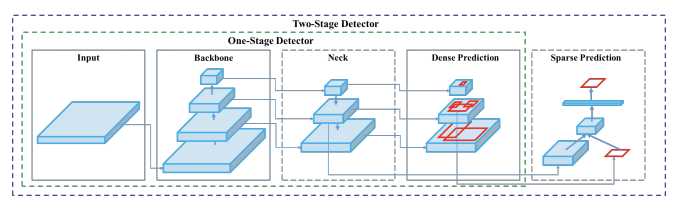
\includegraphics[scale=0.4]{images/yolo-arch.png}
    \caption[แบบจำลอง YOLO]{แบบจำลอง YOLO \cite{img_yolo}}
    \label{fig:yolo-arch}
\end{figure}
\end{itemize}
\begin{table}[!h]
\centering
\caption{YOLOv5 architecture}\label{tbl:yoloarchitech}
\begin{tabular}{p{0.3\textwidth}>{\raggedright\arraybackslash}p{0.6\textwidth}}
\toprule
layers  & Description  \\ \midrule
\textbf{Input} & \\
\quad Input layer: & shape = (batch\_size, 640, 640, 3) \\ 
\textbf{Backbone} & \\
\quad Convolutional layers: & 3x3 filters, stride=2, padding=1, LeakyReLU activation \\
\quad  CSP block (x3): & a series of convolutional layers followed by a concatenation with the input, followed by more convolutional layers \\
\quad  SPP module: & max pooling at multiple scales, followed by convolutional layers \\
\quad  CSP block (x15): & same as previous CSP block, repeated 15 times \\  
\textbf{Neck} & \\
\quad Convolutional layer: & 1x1 filters, stride=1, padding=0, LeakyReLU activation \\
\quad  Upsample layer: & bilinear upsampling, scale factor=2 \\
\quad  Concatenate layer: & concatenates the output of the corresponding CSP block from the backbone with the output of the previous layer \\
\quad  CSP block (x3): & same as previous CSP block, repeated 3 times \\ 
\textbf{Dense prediction} & \\
\quad Convolutional layer: & 3x3 filters, stride=1, padding=1, LeakyReLU activation \\
\quad  Convolutional layer: & 1x1 filters, stride=1, padding=0, linear activation \\
\quad  YOLO detection layer: & predicts bounding boxes, objectness scores, and class probabilities for the corresponding scale \\ 
\textbf{Sparse prediction} & \\ 
\quad Convolutional layer: & 3x3 filters, stride=2, padding=1, LeakyReLU activation \\
\quad  Concatenate layer: & concatenates the output of the corresponding CSP block from the backbone with the output of the previous layer \\
\quad  CSP block (x3): & same as previous CSP block, repeated 3 times \\
\quad  Convolutional layer: & 3x3 filters, stride=1, padding=1, LeakyReLU activation \\
\quad  Convolutional layer: & 1x1 filters, stride=1, padding=0, linear activation \\
\quad  YOLO detection layer: & predicts bounding boxes, objectness scores, and class probabilities for the corresponding scale \\ \hline
\end{tabular}
\end{table}
\begin{itemize}
\pagebreak
\item\textbf{U-Net}
คือหนึ่งโครงข่ายประสาทเทียมที่พัฒนามาจากโครงข่ายประสาทคอนโวลูชัน (Convolutional Neural Network) แบบดั้งเดิม โดยรูปแบบสถาปัตยกรรมของ network นี้มีรูปแบบที่ย่อและขยายข้อมูลในแต่ละ layers ลักษณะคล้ายรูปตัว U ดังรูปภาพที่ \ref{fig:U-Net} มีส่วนประกอบ 3 ส่วน โดยฝั่งซ้ายของแบบจำลองจะเรียกว่า Encoder ตรงกลางของแบบจำลองจะเรียกว่่า Bottleneck และฝั่งขวาของแบบจำลองจะเรียกว่า Decoder ดังตารางที่ \ref{tbl:U-Netarchitech}
โดยแบบจำลองนี้ สามารถระบุพื้นที่และแยกเส้นขอบได้ดี ในระดับ pixel space จึงเหมาะการโจทย์ Image Segmentation หรือ Image Classification โดย input และ output ของ U-Net เป็นขนาดเท่ากัน \cite{UNet} \\
\begin{figure}[!h]\centering
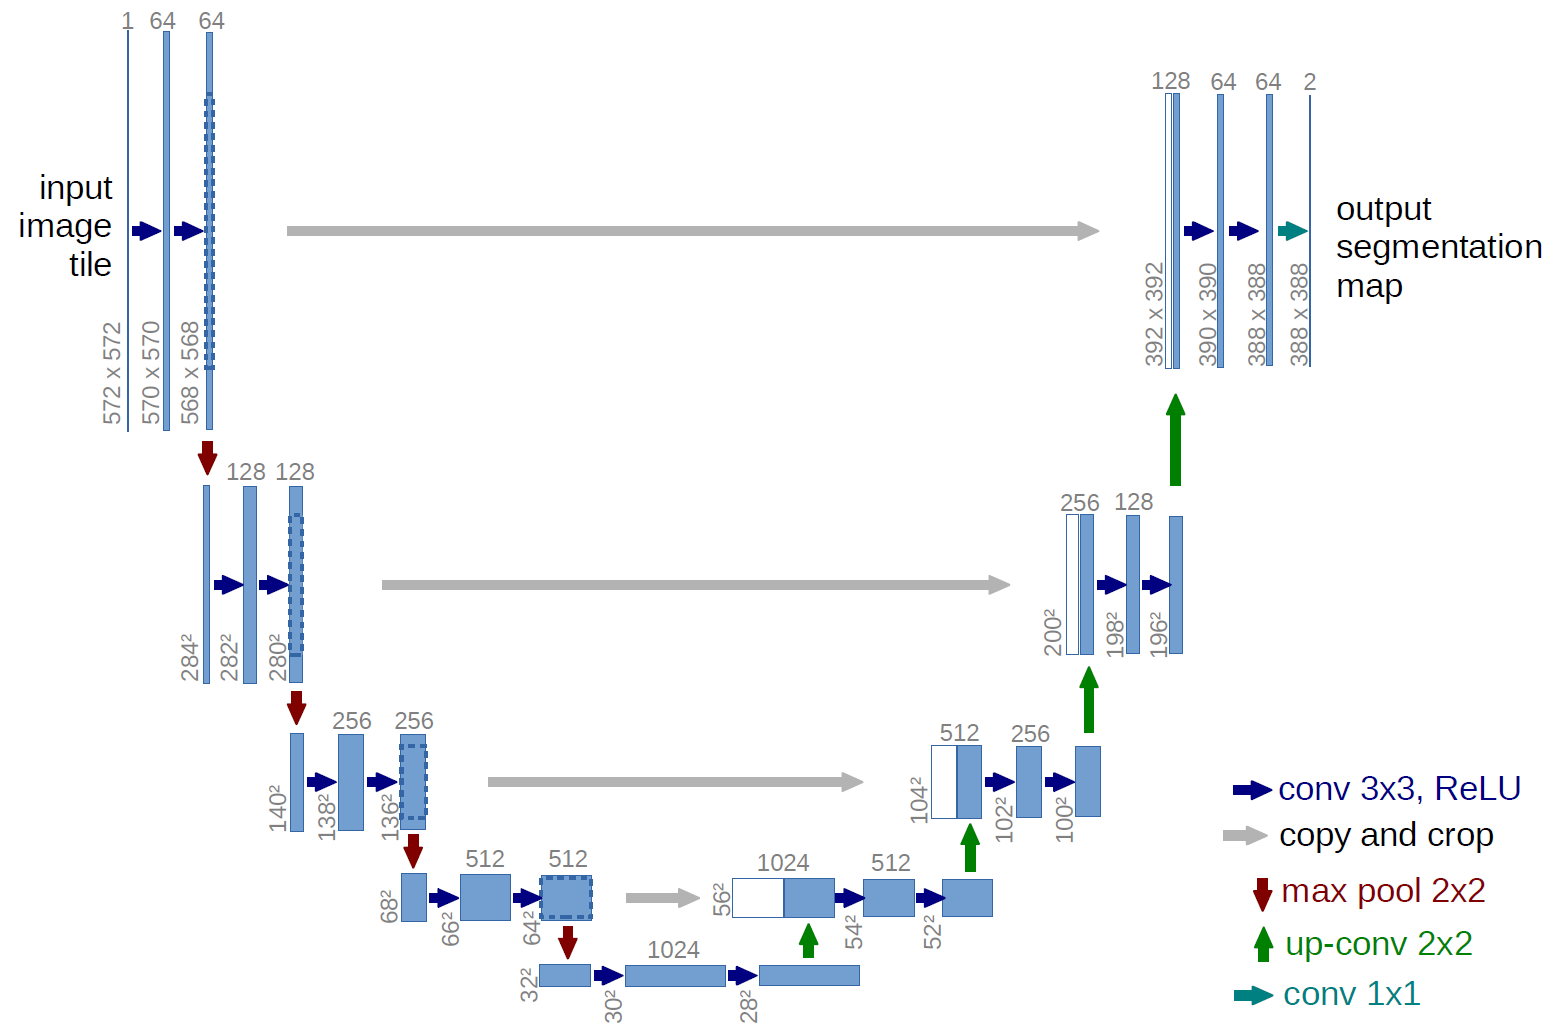
\includegraphics[width=7cm]{images/unetarchitex.png}
\caption[แบบจำลอง U-Net]{แบบจำลอง U-Net \cite{img_unet}} \label{fig:U-Net}
\end{figure}
\pagebreak

\item \textbf{Residual Attention U-Net (RA U-Net)} 
แบบจำลองที่นำคุณสมบัติของ Residual Convolution block แทนการใช้ Convolution block ใน Encoder โดยจะมีโครงสร้างแบบจำลองมีส่วนประกอบดังตารางที่ \ref{tbl:raunetarchitech} และความแตกต่างจะแสดงดังรูปที่ \ref{fig:cv2r} มาใช้ร่วมกับ Attention block แบบจำลองตามโครงสร้างจากงานวิจัยของ Qiangguo Jin และคณะ \cite{RAUNet} แสดงดังรูปที่ \ref{fig:RAUnet-arch}
\begin{figure}[!h]
    \centering
    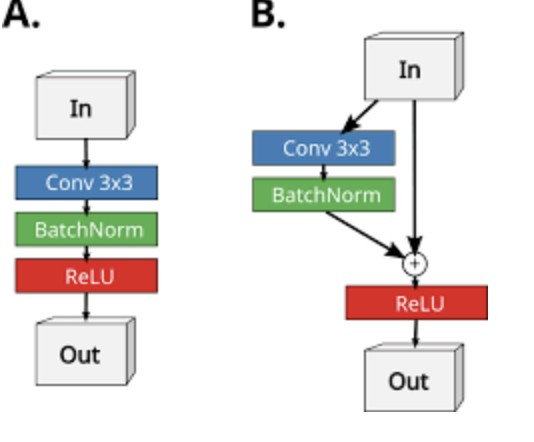
\includegraphics[scale=0.25]{images/cv2d_rs_cv2d.jpg}
    \caption[A. Convolution block, B. Residual Convolution block]{A. Convolution block, B. Residual Convolution block \cite{RAUNet}}
    \label{fig:cv2r}
\end{figure}

\begin{figure}[!h]
    \centering
    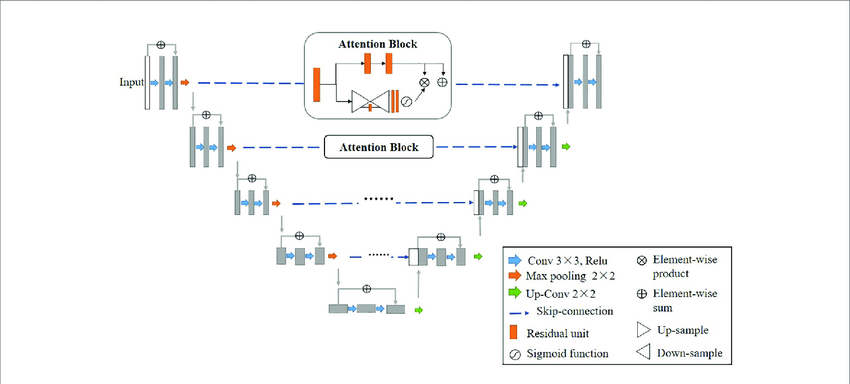
\includegraphics[scale=0.35]{images/Architecture-of-residual-attention-U-net-RA-Unet.png}
    \caption[แบบจำลอง Residual Attention U-Net]{แบบจำลอง Residual Attention U-Net \cite{RAUNet}}
    \label{fig:RAUnet-arch}
\end{figure}
\pagebreak

\begin{table}[!h]
\centering
\caption{U-Net architecture}\label{tbl:U-Netarchitech}
\begin{tabular}{p{0.3\textwidth}>{\raggedright\arraybackslash}p{0.6\textwidth}}
\toprule
layers  & Description  \\ \midrule
\textbf{Input Stage:} & \\
\quad Input layer: & shape = (batch\_size, 256, 256, 3) \\ 
\textbf{Encoding Stage:} & \\

\quad Convolutional Block: & 64 filters, 3x3 kernel size, ReLU activation, and same padding \\
\quad Max pooling layer: & 2x2 pool size \\
\quad Convolutional Block: & 128 filters, 3x3 kernel size, ReLU activation, and same padding \\
\quad Max pooling layer: & 2x2 pool size \\
\quad Convolutional Block: & 256 filters, 3x3 kernel size, ReLU activation, and same padding \\
\quad Max pooling layer: & 2x2 pool size \\
\quad Convolutional Block: & 512 filters, 3x3 kernel size, ReLU activation, and same padding \\
\textbf{Bottleneck Stage:} & \\
\quad Max pooling layer: & 2x2 pool size \\
\quad Convolutional Block: & 1024 filters, 3x3 kernel size, ReLU activation, and same padding \\
\textbf{Decoding Stage:} & \\
\quad Up-sampling layer: & 2x2 stride \\
\quad Concatenation layer: & corresponding encoding stage layer \\
\quad Convolutional Block: & 512 filters, 3x3 kernel size, ReLU activation, and same padding \\
\quad Up-sampling layer: & 2x2 stride \\
\quad Concatenation layer: & corresponding encoding stage layer \\
\quad Convolutional Block: & 256 filters, 3x3 kernel size, ReLU activation, and same padding \\
\quad Up-sampling layer: & 2x2 stride \\
\quad Concatenation layer: & corresponding encoding stage layer \\
\quad Convolutional Block: & 128 filters, 3x3 kernel size, ReLU activation, and same padding \\
\quad Up-sampling layer: & 2x2 stride \\
\quad Concatenation layer: & corresponding encoding stage layer \\
\quad Convolutional Block: & 64 filters, 3x3 kernel size, ReLU activation, and same padding \\
\quad Output layer: & appropriate number of filters and activation function \\

\hline
\end{tabular}
\end{table}

\begin{table}[!h]
\centering
\caption{RA U-Net architecture}\label{tbl:raunetarchitech}
\begin{tabular}{p{0.3\textwidth}>{\raggedright\arraybackslash}p{0.6\textwidth}}
\toprule
layers  & Description  \\ \midrule
\textbf{Input Stage:} & \\
\quad Input layer: & shape = (batch\_size, 256, 256, 3) \\ 
\textbf{Encoding Stage:} & \\
\quad Residual Convolutional Block: &  64 filters, 3x3 kernel size, and ReLU activation \\
\quad Max pooling Layer: & 2x2 pool size \\
\quad Residual Convolutional Block: &  128 filters, 3x3 kernel size, and ReLU activation \\
\quad Max pooling Layer: &  2x2 pool size \\
\quad Residual Convolutional Block: &  256 filters, 3x3 kernel size, ReLU activation, and same padding \\
\quad Max pooling Layer: &  max pooling with 2x2 pool size \\
\quad Residual Convolutional Block: &  512 filters, 3x3 kernel size, ReLU activation, and same padding \\
\textbf{Bottleneck Stage:} & \\
\quad Residual Convolutional Block: &  1024 filters, 3x3 kernel size, ReLU activation, and same padding \\
\textbf{Decoding Stage:} & \\
\quad Up-sampling layer: &  bilinear interpolation with 2x up-sampling factor \\
\quad Concatenation layer: &  corresponding encoding stage layer \\
\quad Residual Convolutional Block: &  512 filters, 3x3 kernel size, ReLU activation, and same padding \\
\quad Up-sampling layer: &  bilinear interpolation with 2x up-sampling factor \\
\quad Concatenation layer: &  corresponding encoding stage layer \\
\quad Residual Convolutional Block: &  256 filters, 3x3 kernel size, ReLU activation, and same padding \\
\quad Up-sampling layer: &  bilinear interpolation with 2x up-sampling factor \\
\quad Concatenation layer: &  corresponding encoding stage layer \\
\quad Residual Convolutional Block: &  128 filters, 3x3 kernel size, ReLU activation, and same padding \\
\quad Up-sampling layer: &  bilinear interpolation with 2x up-sampling factor \\
\quad Concatenation layer: &  corresponding encoding stage layer \\
\quad Residual Convolutional Block: &  64 filters, 3x3 kernel size, ReLU activation, and same padding \\
\textbf{Output Stage:} & \\
\quad Convolutional layer: &  appropriate number of filters and 1x1 kernel size \\
\quad Output layer: &  appropriate activation function \\
\hline
\end{tabular}
\end{table}
\item\textbf{Image Augmentation} คือเทคนิคในการเพิ่มจำนวนชุดข้อมูลซึ่งจะช่วยแก้ปัญหาในกรณีที่ชุดข้อมูลมีขนาดน้อยเกินไป ส่งผลให้เกิดการ over-fit ได้ ในการทำ Image Augmentation สามารถทำได้หลากหลายแบบ เช่น Zoom, Shear, Rotate, Flip และ Preprocessing function อื่นๆ ดังรูปภาพที่ \ref{fig:imgaug}
\begin{figure}[!h]
    \centering
    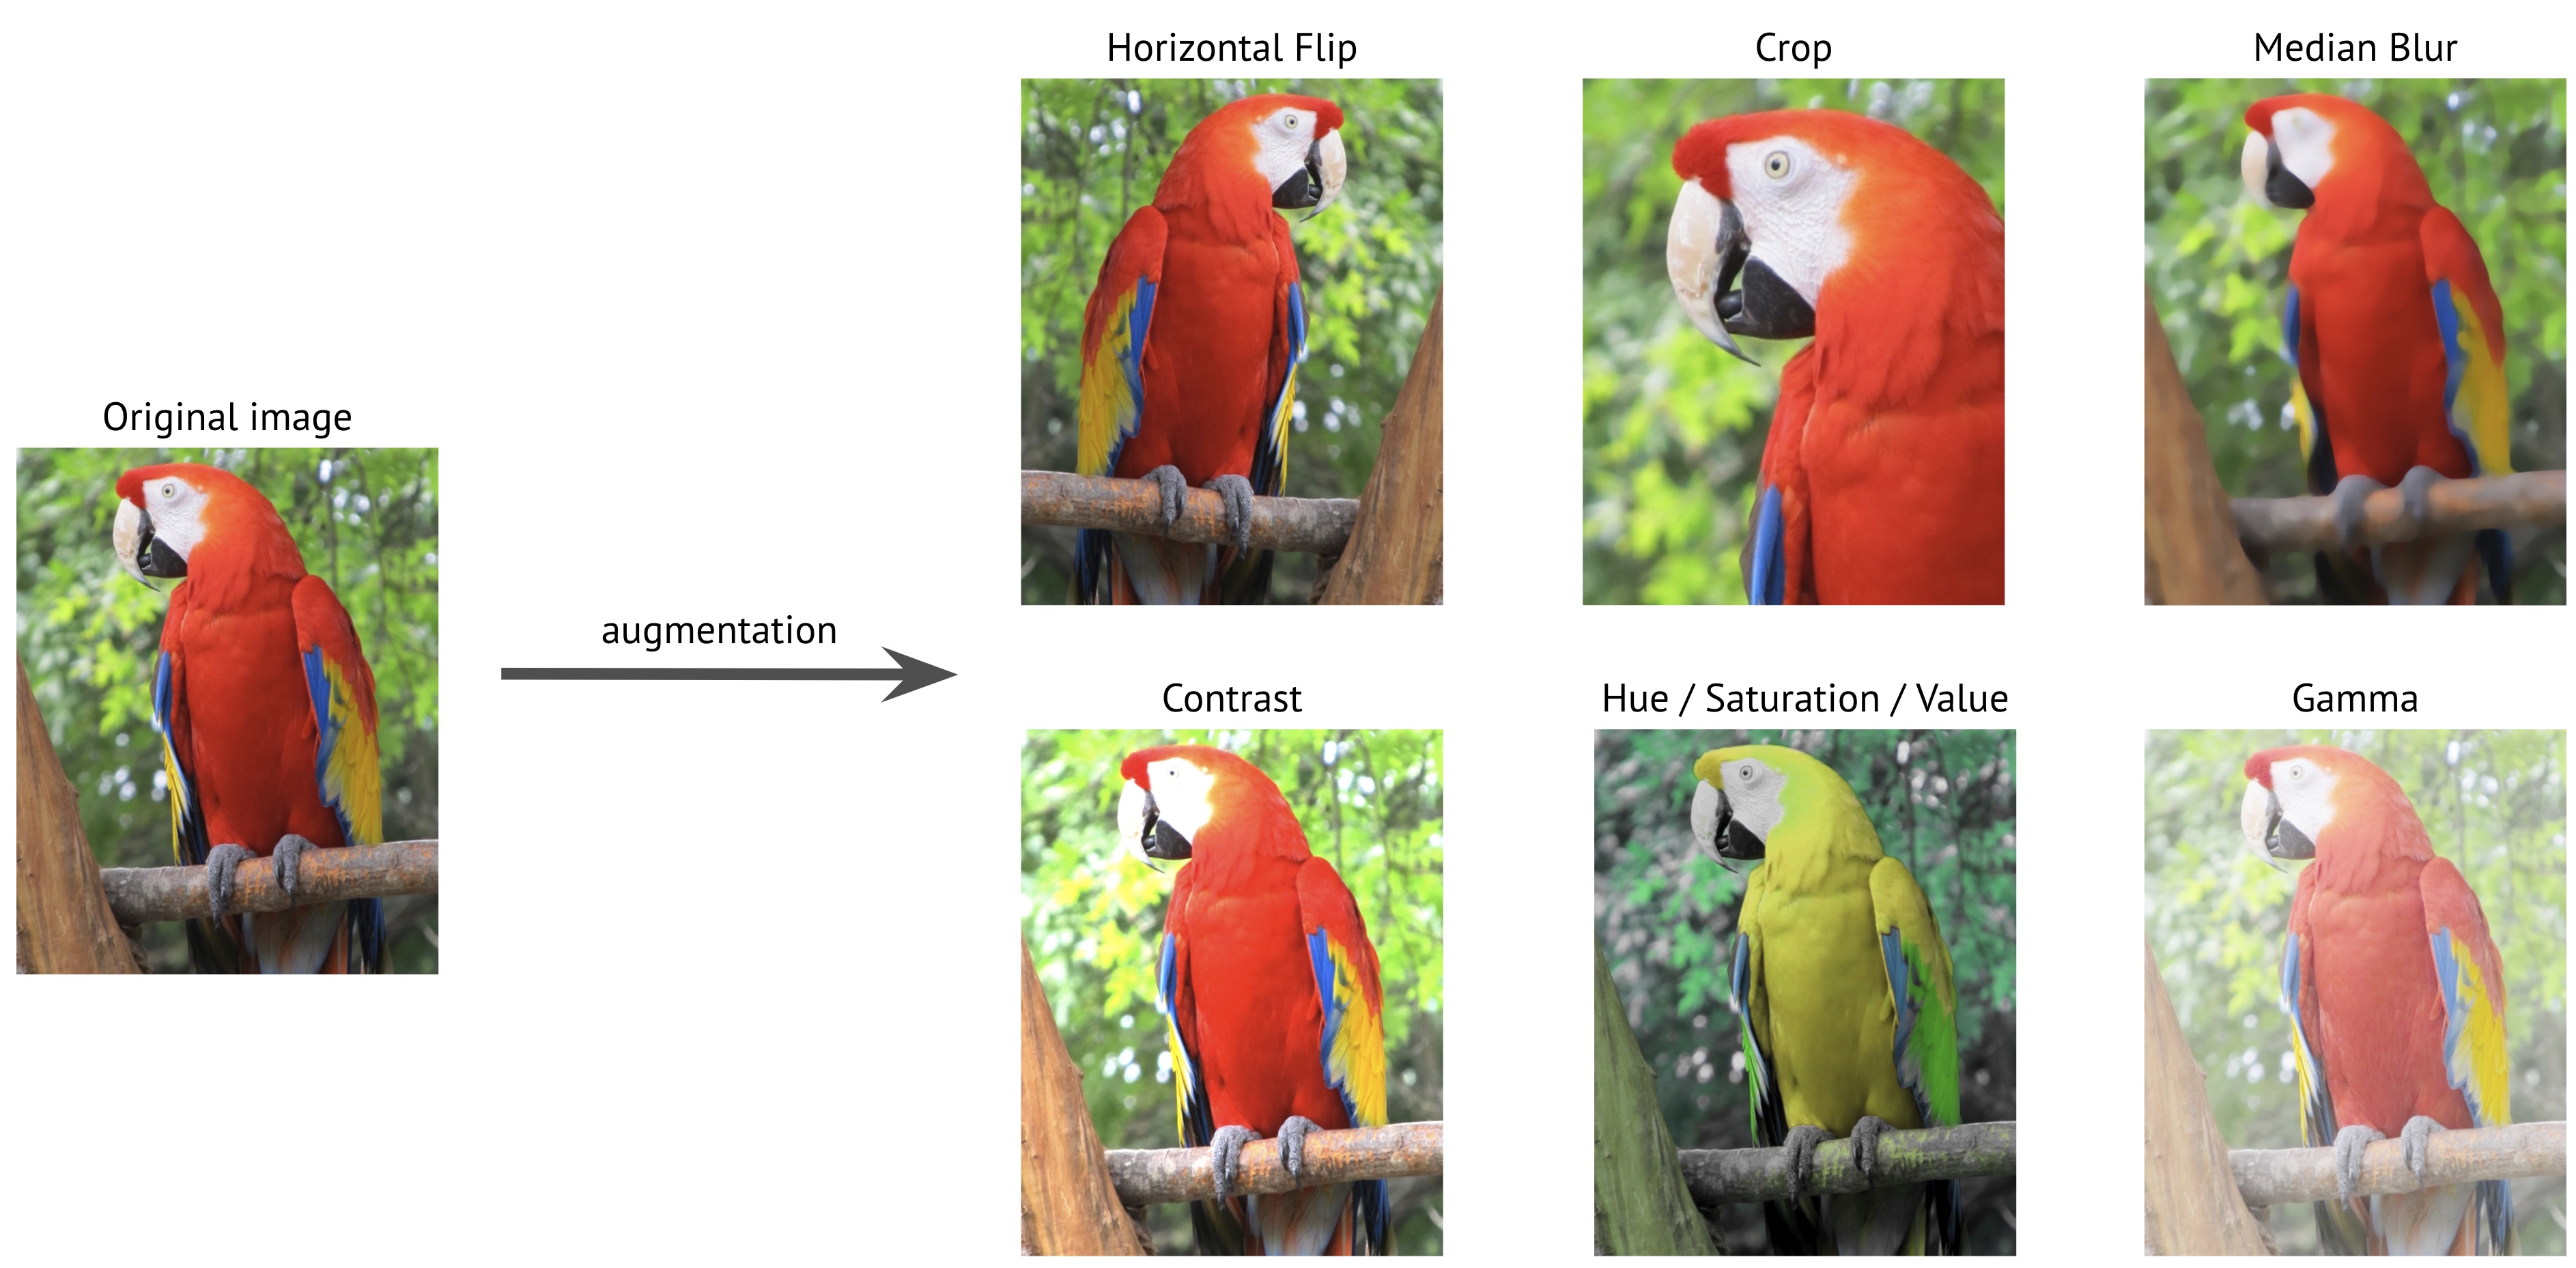
\includegraphics[scale=0.05]{images/augmentation.jpg}
    \caption[Image Augmentation]{Image Augmentation \cite{img_augment}}
    \label{fig:imgaug}
\end{figure}
\end{itemize}
\pagebreak
\section{ภาษาคอมพิวเตอร์และเทคโนโลยี}
\subsection{Python}
ภาษาการเขียนโปรแกรมที่ใช้อย่างแพร่หลายในเว็บแอปพลิเคชัน การพัฒนาซอฟต์แวร์ Data Science และการเรียนรู้ด้วยเครื่องเนื่องจากมีประสิทธิภาพสูง เรียนรู้ง่าย และสามารถทำงานบนแพลตฟอร์มต่าง ๆ ได้มากมาย ทั้งนี้ซอฟต์แวร์ ไพทอนสามารถดาวน์โหลดได้ฟรี ผสานการทำงานร่วมกับระบบทุกประเภท และเพิ่มความเร็วในการพัฒนา \cite{25}
\subsection{OpenCV}
ไลบรารีฟังก์ชันการเขียนโปรแกรมแบบข้ามแพลตฟอร์ม  โดยจะมีเป้าหมายไปที่การแสดงผลด้วยคอมพิวเตอร์แบบเรียลไทม์โดย OpenCV ถูกพัฒนาขึ้นโดย Intel และสามารถใช้งานได้ฟรีภายใต้ ลิขสิทธิ์ของ BSD แบบ Open Source โดยตัว OpenCV ยังรองรับ Deep Learning Framework เช่น TensorFlow, Torch, PyTorch เป็นต้น \cite{26}
\subsection{Scikit-image}
เป็นไลบรารี่การประมวลผลภาพที่นำอัลกอริทึมและเครื่องมือต่างๆที่จำเป็นสำหรับการวิจัย, การศึกษา และ การนำไปใช้จริง สามารถใช้งานได้ฟรีภายใต้ ลิขสิทธิ์ของ BSD แบบ Open Source \cite{scikit-image}
\subsection{Streamlit}
Open-Source Python Library ที่ใช้ในการสร้าง Custom Web Applications ที่มีประสิทธิภาพ ที่ไม่จำเป็นต้องใช้ Libraries API (เช่น Flask หรือ Django) เป็นตัวช่วยในการติดต่อ ทำให้สามารถเขียน Web Application ได้โดยตรงทำให้เหมาะสำหรับ Data Science และ Machine Learning \cite{27}
\subsection{PyTorch}
เป็นหนึ่งใน Library ของ Deep Learning ที่มีประสิทธิภาพสูง เน้นที่การใช้งานที่มีประสิทธิภาพและมีความเร็ว โดย PyTorch ถูกออกแบบจากหลักการเขียนโปรแกรมที่ imperative และ Pythonic เป็นรูปแบบการเขียนโค้ดที่เป็นส่วนเสริมให้ PyTorch ง่ายต่อการดีบัก และง่ายต่อการเชื่อมกับไลบรารีคอมพิวเตอร์อื่นๆ โดย PyTorch ยังคงมีประสิทธิภาพและสนับสนุนการเพิ่มความเร็วของฮาร์ดแวร์ เช่น GPU 
 \cite{NEURIPS2019_bdbca288}

 \subsection{TensorFlow}
 TensorFlow เป็นระบบการเรียนรู้ของเครื่องที่ทํางานได้หลากหลายและในสภาพแวดล้อมที่แตกต่างกัน แบบจำลองการคํานวณขึ้นอยู่กับกราฟ data-flow ที่มีสถานะที่ไม่แน่นอน TensorFlow รองรับแอปพลิเคชันที่หลากหลาย แต่จะมีประสิทธิภาพสูงเมื่อนำไปใช้กับ train เฉพาะจุด  และการใช้ deep neural networks โดย TensorFlow ทําหน้าที่เป็นแพลตฟอร์มสําหรับการวิจัยและการปรับใช้ระบบการเรียนรู้ของเครื่องในหลาย ๆ ด้าน เช่น การรู้จําเสียงพูด คอมพิวเตอร์วิทัศน์ หุ่นยนต์ การดึงข้อมูล และการประมวลผลภาษาธรรมชาติ 
  \cite{tensor}

\subsection{Docker}
Docker เป็นโครงการคอนเทนเนอร์แบบเปิดตามภาษา Go ระบบปฏิบัติการ Linux หลักทั้งหมดรองรับ Docker แนวคิดหลักของเทคโนโลยี Docker คือ Containerization หรือ การตระหนักถึง "สร้าง จัดส่ง และเรียกใช้แอปใดก็ได้ ทุกที่"นั่นคือ การจัดการวงจรชีวิตของแอปพลิเคชันเป็นระยะๆ เพื่อให้บรรลุวัตถุประสงค์ของการบรรจุครั้งเดียวและทํางานทุกที่ \cite{docker}

\subsection{Google Cloud Platform (GCP)}
GCP เป็น ผู้ให้บริการ Cloud Services เช่นเดียวกับ Amazon Web Services (AWS) และ Microsoft Azure ผู้ใช้งานสามารถเข้าใช้งานบริการต่างๆ เช่น พื้นที่จัดเก็บข้อมูล, databases, VM, AI platform และอื่นๆ \cite{googlecloudplatform}

\subsection{Cloud Run}
Cloud Run เป็นบริการหนึ่งใน GCP โดยมีวัตถุประสงค์เพื่อเป็น Serverless ด้วยความสามารถในการ Build และ Deploy แอพพลิเคชันที่มีพื้นฐานการพัฒนาแบบ Containerization \cite{cloudrun}

\subsection{Firebase}
Firebase หรือ Google Firebase เป็นแพลตฟอร์มการพัฒนาแอปที่ช่วยให้สร้างและขยายแอปไปยังผู้ใช้ ซึ่งสนับสนุนโดย GCP ซึ่ง Firebase ช่วยให้นักพัฒนาสามารถพัฒนานาเว็บแอปพลิเคชัน และแอปพลิเคชั่นทั้งใน IOS และAndroid อีกทั้ง Firebase มีเครื่องมือสําหรับติดตามการวิเคราะห์ การรายงาน แก้ไขข้อขัดข้องของแอป การสร้างการทดสอบการตลาดและผลิตภัณฑ์ นอกจากนั้นยังได้รับความไว้วางใจจากธุรกิจนับล้านทั่วโลก \cite{fb}
\pagebreak
\section{ทบทวนวรรณกรรม}
โดยตารางสรุปงานวิจัยที่ใช้การเรียนรู้เชิงลึก (Deep Learning) สามารถดูได้ในตารางที่ \ref{tbl:deeplearn} และในส่วนตารางสรุปงานวิจัยที่ใช้การประมวลผลภาพ (Image Processing) สามารถดูได้ในตารางที่ \ref{tbl:image processing}
\subsection{DeepHCS++: Bright-field to fluorescence microscopy image conversion using multi-task learning with adversarial losses for label-free high-content screening}
 งานวิจัยของ Gyuhyun Lee และคณะ \cite{28} ได้ศึกษาวิธีการแปลภาพถ่ายเรืองแสงจากกล้องจุลทรรศน์ส่องสว่าง ที่แตกต่างกันสามภาพเพื่อสังเกตการตายของนิวเคลียส, นิวเคลียส และไซโตพลาสซึมของนิวเคลียส โดย end-to-end CNN สามารถสร้างภาพถ่ายเรืองแสงจากกล้องจุลทรรศน์ส่องสว่างให้มีความคล้ายกับภาพถ่ายกล้องจุลทรรศน์เรืองแสง โดย Gyuhyun Lee เพิ่มแบบจำลอง multi-task learning กับ adversarial losses เพื่อเป็นการสร้างภาพจำลองที่มีความแม่นยำและสมจริงยิ่งขึ้น และGyuhyun Lee ประเมินประสิทธิภาพของแบบจำลองโดยใช้ชุดภาพถ่ายจากกล้องจุลทรรศน์แบบส่องสว่างและภาพถ่ายจากกล้องจุลทรรศน์แบบเรืองแสง และตรวจสอบความถูกต้องของวิธีการด้วยเมตริกต่าง ๆ ดังนี้ cell number correlation (CNC), peak signal-to-noise ratio (PSNR), structural similarity index measure (SSIM), cell viability correlation (CVC), error maps, และ R$^2$ correlation.

 งานวิจัยนี้ทำการวิจัยในภาพถ่ายเรืองแสงจากการแปลงภาพถ่ายจากกล้องจุลทรรศน์ส่องสว่าง  ดังรูปภาพที่ \ref{fig:DeepHCS} เพื่อให้ได้ภาพถ่ายเรืองแสงที่คล้ายกับภาพถ่ายที่ออกมาจากกล้องจุลทรรศน์เรืองแสง จาก glioblastoma cells และ cell lines of lung adenocarcinoma ซึ่งแตกต่างกับงานของคณะผู้วิจัยที่จะตรวจจับจากภาพถ่ายเนื้อเยื่อผิวหนัง แต่งานวิจัยของ Gyuhyun Lee ภาพถ่ายจะถูกย้อมสีด้วย DAPI ซึ่งมีความคล้ายกับงานวิจัยของคณะผู้วิจัย
 \begin{figure}[!h]
    \centering
    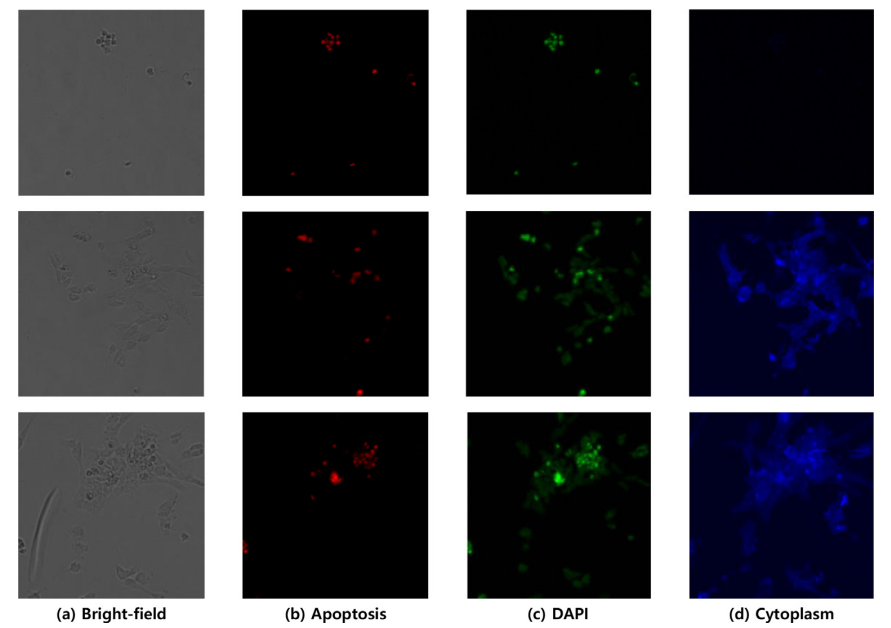
\includegraphics[scale=0.35]{images/paper-deepHDS+.png}
    \caption[รูปตัวอย่างจากเปเปอร์ DeepHCS]{ตารางแสดงรูปตัวอย่างภาพถ่ายสารเรืองแสง โดยแต่ละแถวจะแสดงพื้นที่ที่สนใจ (a) ภาพที่ถ่ายด้วยกล้องจุลทรรศน์แบบไม่มีเครื่องหมายของโปรตีน (b) ภาพสารเรืองแสง apoptosis เพื่อตรวจจับเซลล์ที่ตายแล้ว (c) ภาพเรืองแสง DAPI สำหรับนิวเคลียสของเซลล์ และ (d) ภาพสารเรืองแสงของไซโทรพลาสซึม สำหรับดูลักษณะรูปร่างของเซลล์}
    \label{fig:DeepHCS}
\end{figure}
\subsection{Tox\_(R)CNN: Deep learning-based nuclei profiling tool for drug toxicity screening}
งานวิจัยของ  Daniel Jimenez-Carretero และคณะ \cite{29} ได้ศึกษาความเป็นพิษของยาเป็นปัจจัยสำคัญในการพัฒนายา โดยนิวเคลียสจะถูกย้อมด้วยสารเรืองแสงเพื่อใช้ในการทำนายความเป็นพิษจากการจดจำลักษณะรูปแบบนิวเคลียส  ซึ่งการเรียนรู้เชิงลึกจะทำให้สามารถจำแนกรูปภาพแบบที่มีความซับซ้อนได้อย่างมีประสิทธิภาพมากยิ่งขึ้น และการใช้โครงข่ายประสาทแบบคอนโวลูชัน (deep convolutional neural networks) ถูกนำมาใช้ทำนายความเป็นพิษจากภาพนิวเคลียสที่ย้อมด้วย DAPI และแบบจำลอง nuclei-cropping-based Tox\_CNN สามารถนำมาใช้ในการจำแนกนิวเคลียส รวมถึงการดึงข้อมูลคุณลักษณะโดยอัตโนมัติและจัดกลุ่มสารประกอบตามกลไกการทำงานของยา นอกจากนี้ มีการใช้ fully automated region-based CNNs (RCNN) เพื่อตรวจจับและทำการจำแนกนิวเคลียส โดยให้ผลการทำนายความเป็นพิษของยาจากภาพได้ผลลัพธ์ที่มีความไวสูงและมีความจำเพาะสูง แบบจำลองนี้สามารถนำมาใช้สำหรับการจัดลำดับความสำคัญของการแสดงออกของยา และอาจเพิ่มประสิทธิภาพในการค้นคว้ายาได้ 

งานวิจัยนี้ทำการวิจัยในภาพถ่ายนิวเคลียสที่ถูกย้อมด้วยสารเรืองแสง DAPI ดังรูปภาพที่ \ref{fig:Tox_rcnn} รวมถึงการเลือกใช้แบบจำลองที่จะนำมาใช้เรียนรู้ให้สามารถจำแนกรูปภาพที่มีความซับซ้อนได้ ซึ่งงานวิจัยนี้มีความคล้ายคลึงกับวัตถุประสงค์ที่คณะผู้วิจัยสนใจจะทำการศึกษาคือมีภาพถ่ายนิวเคลียสที่ถูกย้อมด้วยสารเรืองแสง DAPI เช่นเดียวกัน
 \begin{figure}[!h]
    \centering
    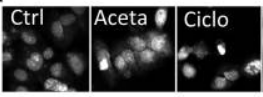
\includegraphics[scale=1]{images/paper-Tox_N(1).png} \\
    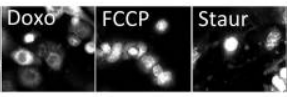
\includegraphics[scale=0.9]{images/paper-Tox_N(2).png}
    \caption[รูปตัวอย่างจากเปเปอร์ Tox\_rcnn]{ตัวอย่างภาพที่ได้จากการถ่ายด้วยกล้องจุลทรรศน์ฟลูออเรสเซนซ์ของเซลล์ที่ย้อมสีด้วย DAPI}
    \label{fig:Tox_rcnn}
\end{figure}
\subsection{A Means of Assessing Deep Learning-Based Detection of ICOS Protein Expression in Colon Cancer}
งานวิจัยของ Md Mostafa Sark และคณะ \cite{30} ได้ศึกษาตัวบ่งชี้ทางชีวภาพ Inducible T-cell COStimulator (ICOS) ที่สามารถระบุการตอบสนองของผู้ป่วยต่อการรักษา การใช้การเรียนรู้เชิงลึกจะสามารถวัดปริมาณของการตรวจตัวบ่งชี้ทางชีวภาพและการตรวจจับนิวเคลียสในสไลด์ IHC ดังรูปภาพที่ \ref{fig:A means}  เพื่อหาปริมาณตัวบ่งชี้ทางชีวภาพของการย้อมสีนิวเคลียส แบบจำลองการแบ่งนิวเคลียสและการตรวจจับ พิสูจน์ได้ว่ามีความแม่นยำมากขึ้นและใช้เวลาน้อยกว่าวิธีการแบบเดิม วิธีการนี้สามารถระบุความหมายเชิงพยากรณ์ของการแสดงออกของโปรตีน ICOS 


 งานวิจัยนี้ทำการวิจัยในภาพ Colorectal cancer เพื่อดูการแบ่งตัวของนิวเคลียสจากการตรวจหาโปรตีน immune-checkpoint ICOS ซึ่งแตกต่างกับงานของคณะผู้วิจัยที่จะตรวจจับนิวเคลียสจากภาพถ่ายเนื้อเยื่อผิวหนังที่ถูกย้อมสีด้วย DAPI ในส่วนที่เป็นนิวเคลียส

 \begin{figure}[!h]
    \centering
    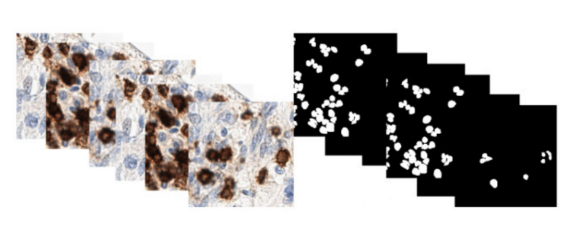
\includegraphics[scale=0.8]{images/paper-Amean.png}
    \caption[รูปตัวอย่างจากเปเปอร์ A means]{ตัวอย่างภาพนิวเคลียสในสไลด์ IHC}
    \label{fig:A means}
\end{figure}
\subsection{Breast Cancer Detection from Histopathology Images Based on YOLOv5}
งานวิจัยของ Wafaa Rajaa Drioua และคณะ \cite{yolopaper} ได้ศึกษาการตรวจหานิวเคลียสของเซลล์ การวิเคราะห์ทางจุลพยาธิวิทยาที่แสดงถึงเซลล์ของตัวอย่างเนื้อเยื่อที่ให้ชุดข้อมูล ซึ่งจําเป็นสําหรับการตรวจหาและระบุลักษณะของมะเร็ง และการเรียนรู้เชิงลึก (Deep learning) แสดงให้เห็นถึงประสิทธิภาพที่มีแนวโน้มในการวินิจฉัยมะเร็งเต้านม ดังนั้นในงานวิจัยนี้ จึงนําเสนออัลกอริทึมการตรวจหาเซลล์ตามแบบจําลอง YOLOv5 ที่เป็นเครือข่าย backbone และถูกนําไปใช้กับชุดข้อมูลสาธารณะของภาพเนื้อเยื่อย้อมสี hematoxylin และ eosin (H\&E) ซึ่งสามารถช่วยแยกนิวเคลียร์ภายในเซลล์  เพื่อประเมินผลการแบ่งจากอัลกอริทึม

 งานวิจัยนี้มีความคล้ายคลึงกับวัตถุประสงค์ที่คณะผู้วิจัยสนใจจะทำการศึกษาคือในส่วนของการตรวจจับนิวเคลียสภายในภาพถ่ายเนื้อเยื่อ แต่งานวิจัยนี้ทำการวิจัยในรูป breast cancer histopathology ที่ถูกย้อมสีด้วย hematoxylin และ eosin (H\&E) ดังรูปภาพที่ \ref{fig:breast} โดยงานของคณะผู้วิจัยจะตรวจจับจากภาพถ่ายเนื้อเยื่อผิวหนังที่ถูกย้อมสีด้วย DAPI

 \begin{figure}[!h]
    \centering
    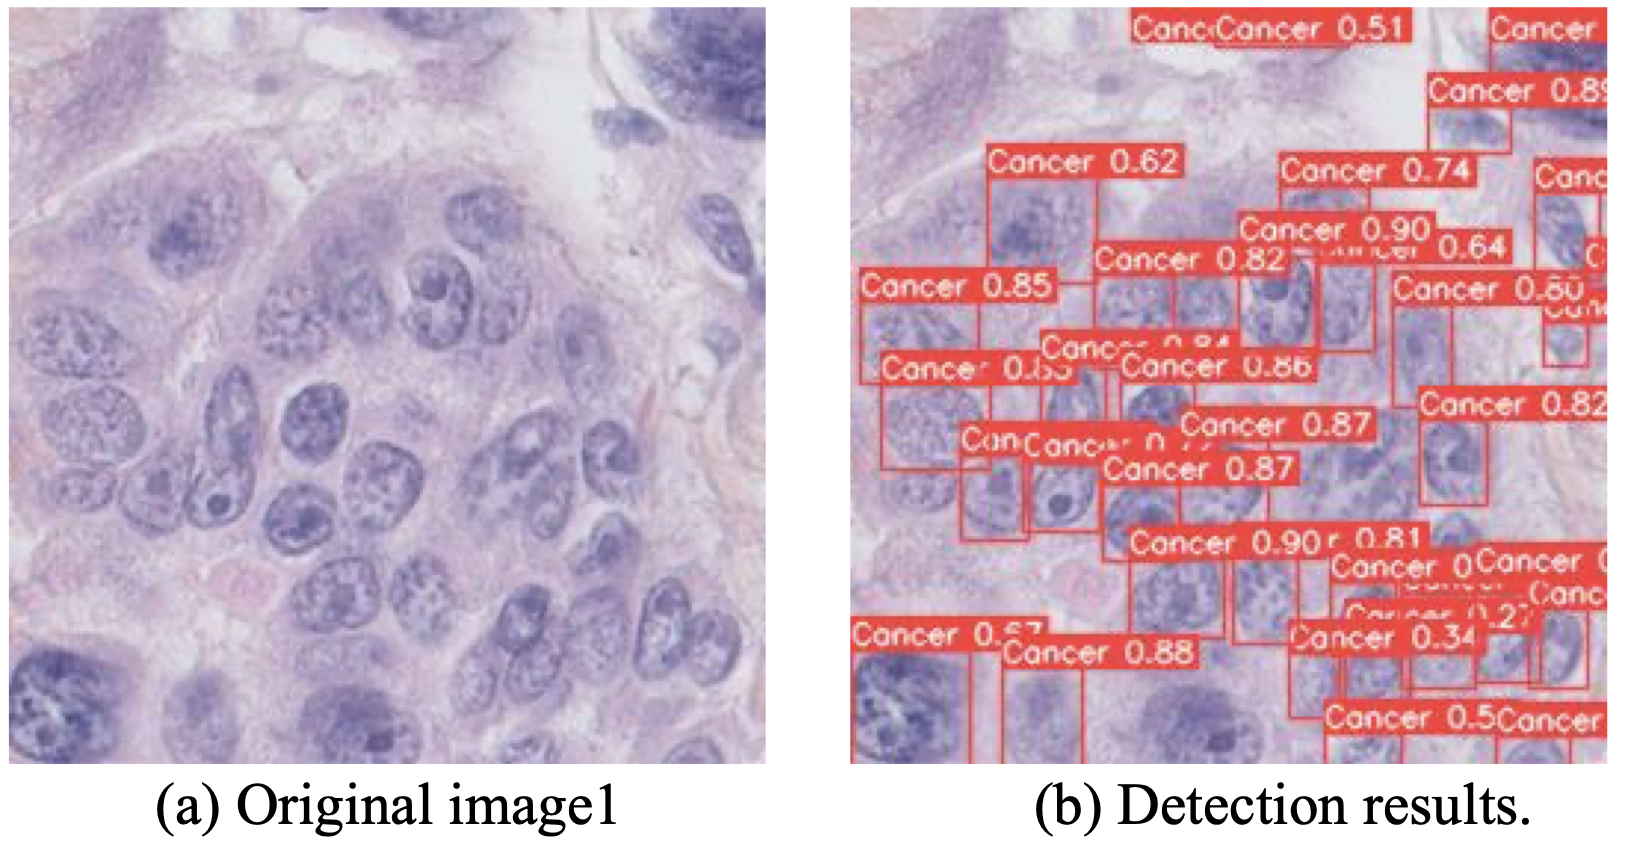
\includegraphics[width=8cm]{images/yolo.png}
    \caption{ตัวอย่างภาพถ่ายนิวเคลียสในงานวิจัยของ Wafaa Rajaa Drioua และคณะ}
    \label{fig:breast}
\end{figure}

\subsection{Automated segmentation of overlapped nuclei using concave point detection and segment grouping}
งานวิจัยของ  Wanjun Zhang และคณะ \cite{31} ได้ทำการประเมินหรือแบ่งส่วนของนิวเคลียสในงานทางชีววิทยา โดยวัตถุประสงค์คือการแบ่งนิวเคลียสที่มีการทับซ้อนกัน ในงานวิจัยนี้นำเสนอวิธีการทั้ง 4 ขั้นตอน ประกอบด้วย การสกัดหาขอบของวัตถุ (Contour Extraction), การหาส่วนเว้าโค้ง (Concave Point Detection), การจัดกลุ่มของขอบวัตถุ (Contour Segment Grouping) และ การวงตำแหน่งนิวเคลียส (Ellipse Fitting) ดังรูปภาพที่ \ref{fig:automated segment}  ซึ่งการจะแบ่งภาพถ่ายนิวเคลียสที่มีความเบลอออกจากกันและภาพถ่ายนิวเคลียสที่หาขอบได้ยากเป็นปัญหาหลักในการแบ่งนิวเคลียสอยู่เสมอ โดยการลดระดับความเบลอด้วยพารามิเตอร์สามารถเพิ่มความแม่นยำในการแบ่งนิวเคลียสที่มีความเบลอออกจากกันได้ และมีการเสนอวิธีการแบ่งด้วยจุดตัดเว้าโค้งในกลุ่มนิวเคลียส ในการสกัดหาส่วนเว้าโค้งของนิวเคลียสที่เห็นได้ชัดเจนและไม่ชัดเจน 
 \begin{figure}[!h]
    \centering
    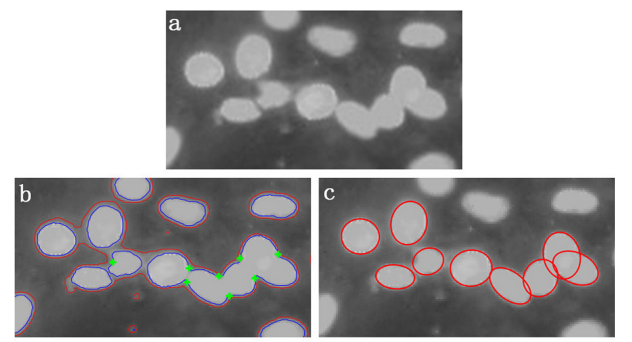
\includegraphics[scale=0.8]{images/paper-Automated segmentation.png}
    \caption[รูปตัวอย่างจากเปเปอร์ automated segment]{ตัวอย่างวิธีการแยกนิวเคลียสที่มีการซ้อนทับกัน โดย (a) รูปภาพต้นฉบับ (b) การสกัดรูปร่างและจุดเว้าของนิวเคลียส (c) ผลลัพธ์ที่ได้}
    \label{fig:automated segment}
\end{figure}
\subsection{Automated image processing workflow for morphological analysis of fluorescence microscopy cell images}
งานวิจัย Sven P. Voigt และคณะ \cite{32} การวิเคราะห์ภาพด้วยคอมพิวเตอร์ของนิวเคลียสและเนื้อเยื่อทางชีวภาพเป็นส่วนเสริมที่จำเป็นสำหรับกล้องจุลทรรศน์ที่มีความเร็วสูง ที่จะช่วยให้นักวิจัยสามารถวิเคราะห์ข้อมูลภาพถ่ายนิวเคลียสที่มีปริมาณมากได้อย่างมีประสิทธิภาพ การศึกษานี้นำเสนอเวิร์กโฟลว์ใหม่สำหรับการวิเคราะห์ผลแบบอัตโนมัติของภาพถ่ายจากกล้องจุลทรรศน์ฟลูออเรสเซนซ์ ซึ่งได้ประโยชน์จากการรันเวิร์กโฟลว์ที่มีการแบ่งส่วนออกเป็นหลาย ๆ ส่วนและนำมารวมเข้าด้วยกันเพื่อสร้างการแบ่งส่วนสุดท้ายที่ดีที่สุด ซึ่งมีการทดสอบโดยใช้ชุดข้อมูลของภาพนิวเคลียสที่ได้จากกล้องจุลทรรศน์ฟลูออเรสเซนซ์ จำนวน 42 นิวเคลียส ประเมินเทียบกับชุดข้อมูลที่แบ่งส่วนด้วยมือ โดยทำการประเมินผลด้วยวิธี F1 score และเปรียบเทียบกับเวิร์กโฟลว์การแบ่งส่วนเดียวซึ่งทำหน้าที่เป็นตัวควบคุม ค่าความแม่นยำและความน่าเชื่อถือของเวิร์กโฟลว์ใหม่นั้นแสดงให้เห็นแล้วว่ามีความสามารถมากกว่าเวิร์กโฟลว์แบบควบคุม ซึ่งได้ค่า F1 score ที่ 0.845 และ 0.608 ตามลำดับ


\subsection{Automated cell counting and cluster segmentation using concavity detection and ellipse fitting techniques}
งานวิจัยของ onal Kothari และคณะ \cite{33} การศึกษานี้เป็นการนำเสนอวิธีการใหม่ ที่มีความรวดเร็ว และกึ่งอัตโนมัติสำหรับการแบ่งกลุ่มนิวเคลียสและการนับจำนวนนิวเคลียสของตัวอย่างภาพเนื้อเยื่อที่มีความแม่นยำ ซึ่งในทางพยาธิวิทยา ส่วยใหญ่มักจะพบกลุ่มนิวเคลียสที่มีความซับซ้อน ซึ่งพบได้ในตัวอย่างเนื้อเยื่อ การแบ่งกลุ่มของคลัสเตอร์เหล่านี้ที่เป็นเรื่องยากสำหรับการพัฒนาวิธีการนับจำนวนนิวเคลียสให้มีความแม่นยำ ดังนั้นเราจึงแก้ไขปัญหาการแบ่งกลุ่มคลัสเตอร์โดยทำตามขั้นตอนสามขั้นตอนนี้ คือ ขั้นตอนแรกจะเกี่ยวข้องกับการประมวลผลล่วงหน้าที่จำเป็น เพื่อให้ได้ภาพขอบเขตของคลัสเตอร์นิวเคลียสที่เหมาะสมจากตัวอย่างเนื้อเยื่อ RGB ขั้นตอนที่สองเกี่ยวข้องกับการตรวจจับความเว้าที่ขอบของคลัสเตอร์เพื่อค้นหาจุดที่ทับซ้อนกันระหว่างสองนิวเคลียส ขั้นตอนที่สามเกี่ยวข้องกับการแบ่งส่วนที่เว้าเหล่านี้โดยใช้เทคนิคการวงรีแบบพอดี เมื่อแบ่งกลุ่มแล้ว แต่ละนิวเคลียสจะถูกนำมานับเพื่อให้ได้จำนวนนิวเคลียส ดังนั้น วิธีการนี้ได้รับการทดสอบกับตัวอย่างเนื้อเยื่อมะเร็ง 4 ชนิดที่แตกต่างกัน และแสดงผลลัพธ์ที่มีเปอร์เซ็นต์ความผิดพลาดต่ำ true positive rate ที่สูง และ false discovery rate ต่ำ

\begin{sidewaystable}
    \centering
\caption{ตารางสรุปงานวิจัยที่ใช้ Deep Learning}\label{tbl:deeplearn}
\begin{tabular}[!h]{p{0.35\textwidth}>{\centering}p{0.2\textwidth}>{\raggedright}p{0.3\textwidth}>{\centering\arraybackslash}p{0.1\textwidth}}
\toprule
Papers                                                                                                                                                       & Method    & Dataset        & Accuracy \\ \midrule
DeepHCS++: Bright-field to fluorescence microscopy image conversion using multi-task learning with adversarial losses for label-free high- content screening \cite{28} & CNN       &   
bright-field and fluorescence microscopy image datasets from patient-driven samples of a glioblastoma & 0.91     \\&&&\\
Tox\_(R)CNN: Deep learning-based nuclei profiling tool for drug toxicity screening \cite{29}                                                                          & CNN, R-CNN     &   
datasets of healthy and toxicity affected labeled nuclei    & 0.90      \\&&&\\
A Means of Assessing Deep Learning-Based Detection of ICOS Protein Expression in Colon Cancer\cite{30}                                                                & U-Net, Mask R-CNN &   
immunohistochemistry-stained slides as a basis for quantifying nuclear staining biomarkers
& 0.98     \\&&&\\
Breast Cancer Detection from Histopathology Images Based on YOLOv5\cite{yolopaper}                                                                & YOLOv5 &   
the breast cancer histopathology image dataset (BNS) and the annotated dataset. 
& 0.86     \\ \bottomrule
\end{tabular}\\
    \centering
\caption{ตารางสรุปงานวิจัยที่ใช้ Image Processing}\label{tbl:image processing}
\begin{tabular}[!h]{p{0.25\textwidth}>{\raggedright}p{0.35\textwidth}>{\raggedright}p{0.25\textwidth}>{\centering\arraybackslash}p{0.1\textwidth}}

\toprule
Papers                                                                                                    & Method  & Dataset & Accuracy  \\ \midrule
Automated segmentation of overlapped nuclei using concave point detection and segment grouping   \cite{31}         & 1. Three-phase level set formulation \\2. Candidate point detection \\3. Concave point detection\\4. Segment grouping and Ellipse fitting   & Nucleus images in two kinds of polyacrylamide substrates, there are lots of fuzzy nuclei.      & 0.98      \\&&&\\
Automated Image Processing Workflow for Morphological Analysis of Fluorescence Microscopy Cell Images \cite{32}    & 1. smoothing intensity values and contrast enhancement \\2. local average threshold and remove small objects\\3. generate markers from peaks for separate touching nuclei\\4.reassigning labels and generate relabeled markers    & Fluorescence microscopy images of biological cells, with image variations arising from differences in cell phenotype & 0.85     \\&&&\\
Automated cell counting and cluster segmentation using concavity detection and ellipse fitting techniques \cite{33} &1. Preprocessing \\2. Concavity or Notch Detection \\3. Segmentation    &  H\&E stained tissue images from three subtypes and IHC stained head and neck cancer tissue image      & 0.91      \\ \bottomrule
\end{tabular}
\end{sidewaystable}
\section{ผลิตภัณฑ์ที่เกี่ยวข้อง}
\subsection{An ImageJ plugin for the high throughput image analysis of in vitro scratch wound healing assays}
งานวิจัยของ C. Igathinath และคณะ \cite{34} การศึกษานี้เป็นการพัฒนา plugin ที่ใช้สำหรับโปรแกรม ImageJ เพื่อจดจำขนาดการรักษาบาดแผลแบบ อัตโนมัติ แก้ไขความกว้างของบาดแผลโดยเฉลี่ยโดยพิจารณาจากความเอียงและหาค่าพารามิเตอร์ที่สำคัญอื่นๆ เช่น พื้นที่ เศษส่วนของพื้นที่แผล ความกว้างของแผลเฉลี่ย และส่วนเบี่ยงเบนความกว้างของภาพบาดแผลที่ได้ จากการทดสอบรอยขีดข่วน/การรักษาบาดแผล ในการพัฒนาอัลกอริทึมนี้มีการแบ่งส่วนการมองเห็นด้วย 
คอมพิวเตอร์แบบคลาสสิกที่เน้นการประเมินความแปรปรวนของความเข้มพิกเซลที่อยู่ใกล้เคียงด้วยการ ตรวจสอบอย่างรอบคอบของภาพระดับสีเทาที่ได้จากการทดสอบการสมานของบาดแผล 
\subsection{Shape identification and particles size distribution from basic shape parameters using ImageJ}
งานวิจัยของ  H.S. Kim และคณะ  \cite{35} วัตถุประสงค์ของงานวิจัยนี้คือการวิเคราะห์การกระจายขนาดอนุภาคที่รวดเร็วและแม่นยำ ซึ่งเป็นสิ่งที่ต้องการวิเคราะห์ในด้านเทคนิคต่างๆ ที่จัดการกับวัตถุที่มีขนาดเล็กหรืออนุภาค รวมทั้งการลดขนาด นักวิจัยได้พัฒนาปลั๊กอิน ImageJ ที่แยกมิติออกจากภาพดิจิทัลของวัตถุที่ไม่ปะติดปะต่อกัน หลังจากระบุรูปร่างและกำหนดการกระจายขนาดวัตถุแล้ว นักวิจัยจึงทำการกำหนดแกนหลักและแกนรองของ ImageJ พร้อมกับปัจจัยการแก้ไขที่พัฒนาขึ้นซึ่งกำหนดขนาดของวัตถุได้อย่างมีประสิทธิภาพ งานวิจัยนี้ได้อธิบายการพัฒนาปลั๊กอินและการประยุกต์ใช้กับธัญพืชอาหารและชีวมวลบด โดยใช้คอมพิวเตอร์สร้างรูปทรงเรขาคณิตเป็นวัตถุอ้างอิง กลยุทธ์การระบุรูปร่างที่กล่าวถึงรูปทรงเรขาคณิตทั่วไป เช่น สี่เหลี่ยมจัตุรัส สี่เหลี่ยมจัตุรัสเอียง สี่เหลี่ยมผืนผ้า สี่เหลี่ยมผืนผ้าเอียง วงกลม วงรี และวงรีเอียงได้รับการพัฒนา กลยุทธ์นี้ใช้พารามิเตอร์รูปร่างที่กำหนดใหม่เพียงสามตัวในการระบุวัตถุ เช่น อัตราส่วนส่วนกลับ สี่เหลี่ยม และอัตราส่วนแกนหลัก Feret จากเอาต์พุตมาตรฐานที่สร้างโดย ImageJ การประเมินผลกระทบของรูปร่าง ขนาด และทิศทางของวัตถุบนความเบี่ยงเบนจากความยาวและความกว้างของวัตถุอ้างอิง บ่งชี้ว่าค่าเบี่ยงเบนสัมบูรณ์เฉลี่ยของปัจจัยทั้งหมดเหล่านี้น้อยกว่า 1.3\% ปลั๊กอินที่พัฒนาแล้วถูกนำไปใช้อย่างประสบความสำเร็จในการวิเคราะห์ขนาดและการกระจายขนาดของเมล็ดอาหารและภาพอนุภาคมิสแคนทัสบด ปลั๊กอินนี้สร้างการกระจายขนาดอนุภาคที่รวดเร็วและแม่นยำจากภาพดิจิทัล และสามารถนำไปใช้กับแอปพลิเคชันการวิเคราะห์อนุภาคต่างๆ
\subsection{Columbus Image Data Storage and Analysis System}
งานวิจัยของ PerkinElmer และคณะ \cite{11} ได้อธิบายไว้ว่า Columbus เป็นแพลตฟอร์มที่ใช้ในการจัดเก็บและวิเคราะห์ภาพสำหรับภาพที่มีเนื้อหาหรือรายละเอียดสูง ซึ่งในปัจจุบันมีการใช้แบบจำลองของโรคที่มีความซับซ้อนและสัมพันธ์กันทางสรีรวิทยามากขึ้น เครื่องมือที่มีความซับซ้อนมากขึ้นจึงมีความจำเป็นในการอธิบายนิวเคลียสและฟีโนไทป์ของพวกมันอย่างครอบคลุม แพลตฟอร์ม Columbus เป็นระบบจัดเก็บและวิเคราะห์ข้อมูลภาพเพียงระบบเดียวที่รองรับรูปแบบไฟล์ที่หลากหลาย โดยแพลตฟอร์ม Columbus สามารถเข้าถึงการจัดเก็บ และการสำรวจข้อมูล โดยสามารถนำเข้ารูปภาพจากเครื่องมือสร้างภาพที่มีรายละเอียดสูงสำหรับโซลูชันเดียว สำหรับการจัดเก็บข้อมูลและการวิเคราะห์รูปภาพ และการวิเคราะห์ภาพสำหรับการคัดกรองฟีโนไทป์ สร้างข้อมูลที่มีนัยสำคัญทางสถิติ เชิงปริมาณ และแบบหลายพารามิเตอร์จากภาพนิวเคลียสเพื่อให้ได้ผลลัพธ์ที่มีประสิทธิภาพ \cite{11}
\subsection{Validation and Automation of Phenotypic Profiling Across Multiple Cell Lines}
งานวิจัยของ  D.Y. Eun และคณะ \cite{36} จุดประสงค์ของการสัมมนานี้คือการนำเสนอการทดสอบ Autophagy ในกลุ่มนิวเคลียสมะเร็งทั้งหมด 3 กลุ่ม เพื่อทำการตรวจสอบและทำให้กระกวนการวิเคราะห์ฟีโนไทป์ HCS เป็นไปได้อย่างอัตโนมัติ โดยแพลตฟอร์ม Columbus และ Spotfire High Content Profiler โดยแพลตฟอร์ม Columbus จะเป็นแพลตฟอร์มที่ใช้ในการจัดเก็บข้อมูล จัดการข้อมูล และวิเคราะห์ภาพที่ได้จากเครื่องมือ HCS ทั้งหมด รวมถึงลำดับการวิเคราะห์ที่มีความซับซ้อนก็สามารถวิเคราะห์ได้โดยใช้แนวทางการ Building Block ทำให้ผลลัพธ์จากการวิเคราะห์รูปภาพนั้น สามารถเลือกได้โดยตรงภายใน Spotfire High Content Profiler (HCP) สำหรับการวิเคราะห์และการแสดงภาพข้อมูล HCS แบบหลายพารามิเตอร์ 

\begin{table}[ht!]
% \vspace{-7.5in}
\caption{ตารางสรุปผลิตภัณฑ์ที่เกี่ยวข้อง}\label{tbl:product}
\begin{tabular}{p{0.4\textwidth}>{\centering}p{0.2\textwidth}>{\raggedright\arraybackslash}p{0.35\textwidth}}
\toprule
Papers          & Product    & Limitation \\ \midrule
An ImageJ plugin for the high throughput image analysis of in vitro scratch wound healing assays \cite{34} & ImageJ      &  ใช้เวลาในการประมวลผลนานและจำกัดปริมาณรูปที่สามารถประมวลผลได้     \\&&\\
Shape identification and particles size distribution from basic shape parameters using ImageJ \cite{35} & ImageJ       & ในการวัดค่าจะต้องทำการกำหนดขอบเขตที่จะให้โปรแกรมตรวจหาด้วยตัวเอง     \\
&&\\ Columbus Image Data Storage and Analysis System \cite{11}       & Columbus     & ไม่สามารถหาบริเวณที่นิวเคลียสทรงกลม 2 อันซ้อนทับกันไม่สนิท เพราะทำให้รูปทรงที่มองเห็นไม่เป็นทรงกลมจริง ๆ      \\&&\\
Validation and Automation of Phenotypic Profiling Across Multiple Cell Lines    \cite{36}               & Columbus   & ภาพ Immunofluorescence Tissue ไม่สามารถใช้งานโปรแกรม Columbus ได้     \\ \bottomrule
\end{tabular}
\end{table}

%%%%%%%%%%%%%%%%%%%%%%%%%%%%%%%%%%%%%%%%%%%%%%%%%%%%%55
%%%%%%%%%%%%%%%%%%%%%%%%%%%%%%%%%%%%%%%%%%%%%%%%%%%%%
%%%%%%%%%%%%%%%%%%%%%%%%%%%%%%%%%%%%%%%%%%%%%%%%%%%%%
\chapter{วิธีการดำเนินงาน}
ในบทนี้จะกล่าวถึงภาพรวมการดำเนินงานวิจัยเรื่อง เว็บแอปพลิเคชันสำหรับการตรวจนับนิวเคลียสจากภาพถ่ายเนื้อเยื่อจากการย้อมด้วยสารเรืองแสง รวมถึงวิธีการดำเนินงาน กระบวนการที่จะใช้ในการดำเนินงาน และการออกแบบงานวิจัยโดยมีเนื้อหา ดังนี้ 

\section{รายละเอียดภาพรวมการดำเนินงานวิจัย}
งานวิจัยในครั้งนี้มุ่งเน้นพัฒนาระบบที่สามารถนับจำนวนนิวเคลียสจากภาพถ่ายเนื้อเยื่อจากการย้อมด้วยสารเรืองแสง เพื่อช่วยลดภาระของนักพยาธิวิทยาที่ต้องทำการนับจำนวนนิวเคลียสภายในภาพถ่ายด้วยตนเอง ซึ่งการนับจำนวนนิวเคลียสเองนั้นต้องใช้ความพยายามในการคัดแยกและระยะเวลาต่อหนึ่งภาพที่สูงเป็นอย่างมาก ดังนั้นคณะผู้วิจัยจึงตัดสินใจที่จะออกแบบแนวทางการนับจำนวนของนิวเคลียสภายในภาพถ่ายเนื้อเยื่อจากการย้อมด้วยสารเรืองแสง โดยการดำเนินงานวิจัยจะเริ่มจากการเตรียมภาพและ label ตำแหน่งของนิวเคลียส หลังจากนั้นนำเข้าแบบจำลองทั้ง 4 แบบเพื่อหาแบบจำลองที่ดีที่สุดที่จะนำมาใช้ในการพัฒนาเว็บแอปพลิเคชัน ตามแผนภาพรายละเอียดภาพรวมการดำเนินงานวิจัยดังรูปภาพที่ \ref{fig:Flowchart3}

\begin{figure}[!h]
    \centering
    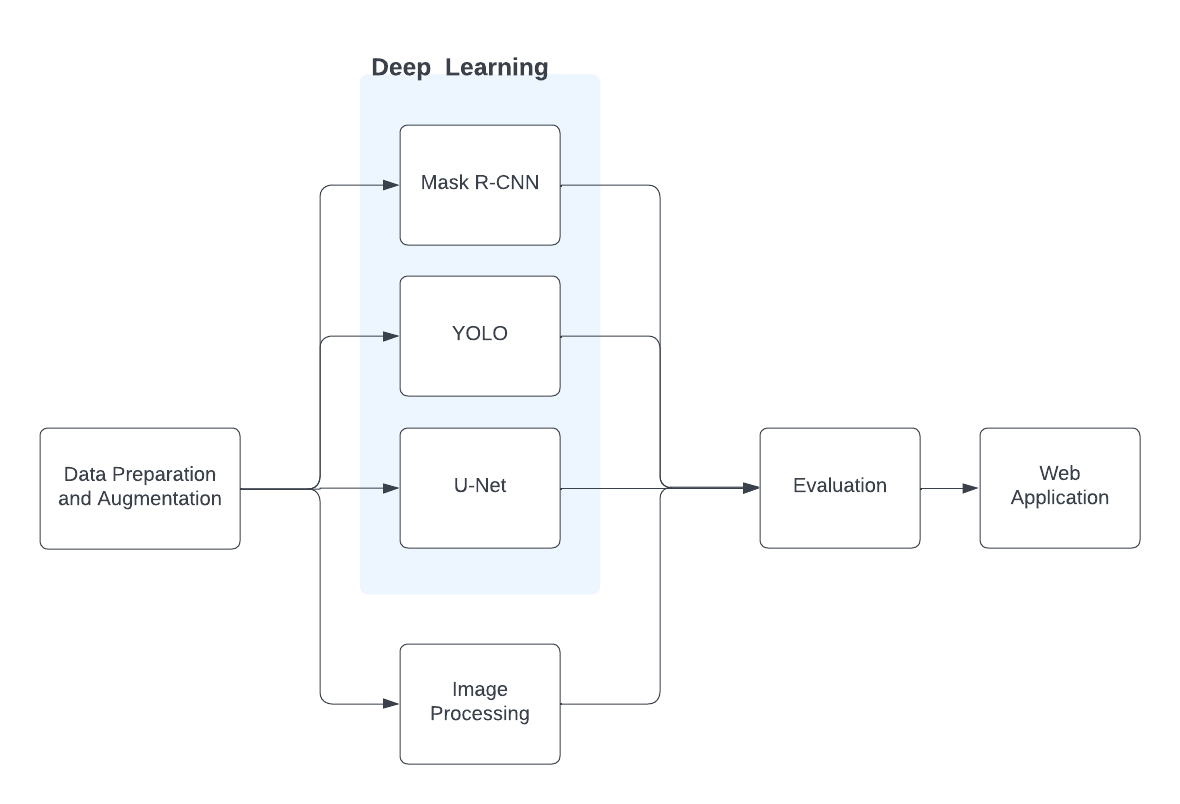
\includegraphics[scale=0.3]{images/Flowchart3.png}
    \caption{แผนภาพรายละเอียดภาพรวมการดำเนินงานวิจัย}
    \label{fig:Flowchart3}
\end{figure}
\section{ความต้องการของนักพยาธิวิทยา}
หลังจากที่คณะผู้วิจัยได้วิเคราะห์ความต้องการของนักพยาธิวิทยาที่ต้องการวิเคราะห์ภาพถ่ายเนื้อเยื่อจากการย้อมด้วยสารเรืองแสง มีรายละเอียดดังนี้
\begin{enumerate}
    \item เว็บแอปพลิเคชันที่สามารถอัปโหลดรูปที่ต้องการวิเคราะห์
	\item จำนวนนิวเคลียสจากภาพถ่ายเนื้อเยื่อจากการย้อมด้วยสารเรืองแสง
	\item ภาพผลลัพธ์ที่มีการ label ตำแหน่งของนิวเคลียส
    \item ตารางสรุปตำแหน่งของนิวเคลียส
    \item สามารถบันทึกรูปภาพผลลัพธ์และตารางสรุปตำแหน่งของนิวเคลียส
\end{enumerate}
\section{การออกแบบระบบซอฟต์แวร์}
\subsection{การพัฒนาแบบจำลองในการนับจำนวนนิวเคลียส}
เนื่องจากงานวิจัยที่ได้ศึกษามามีวิธีการที่ใช้ 2 แบบ ได้แก่ การเรียนรู้เชิงลึก (Deep Learning) และ การประมวลผลภาพ (Image Processing) คณะผู้วิจัยจึงทำการทดลองเปรียบเทียบผลลัพธ์ เพื่อเลือกวิธีที่ดีที่สุดมาใช้เป็นอัลกอริทึมของเว็บแอปพลิเคชัน
% \subsubsection\titleformat{\subsubsection}
% {\makebox[0.5in]{\textbf\thesubsubsection}\textbf{Deep Learning}}

\subsubsection{การเรียนรู้เชิงลึก (Deep Learning)}
จากการศึกษางานวิจัยที่เกี่ยวข้องในตารางที่ \ref{tbl:deeplearn} มีตัวอย่างของงานวิจัยที่ใช้แบบจำลอง Mask R-CNN, YOLO และ U-Net สำหรับนับจำนวนนิวเคลียส คณะผู้วิจัยจึงมีความสนใจที่จะทำการศึกษาและพัฒนาด้วยแบบจำลองเหล่านี้
\begin{itemize}[listparindent=\parindent]
% \setlength{\itemindent}{.3in}
\item \textbf{ชุดข้อมูลที่ใช้ในการพัฒนาแบบจำลอง} 
จากชุดข้อมูลภาพถ่ายเนื้อเยื่อจากการย้อมด้วยสารเรืองแสงทั้งหมด 197 รูป นักพยาธิวิทยาได้ทำการเลือก 5 รูปที่มีขนาด 1920 × 1536 พิกเซล จากนั้นทำการแบ่งเป็นรูปเล็ก ๆ ได้รูปขนาด 319 × 255 พิกเซล เพื่อให้ง่ายต่อการทำ label และลดขนาดของ Neural Network โดยจะแบ่งเป็นรูปละ 36 รูปเล็ก เพราะฉะนั้นจะได้ทั้งหมด 180 รูป เจากนั้นให้นักพยาธิวิทยา label นิวเคลียสภายในรูป ดังรูปที่ \ref{fig:img_train} ต่อมาผู้วิจัยได้นำรูปที่มีพื้นหลังสีดำซึ่งไม่มีนิวเคลียสภายในรูปออกจากชุดข้อมูลทั้งหมด ซึ่งเหลือผลลัพธ์ทั้งหมดจำนวน 122 รูป ค่าเฉลี่ยจำนวนนิวเคลียสในแต่ละรูปคือ 26 เซลล์ ผู้วิจัยได้ทำการแบ่งชุดข้อมูลจากกระบวนการก่อนหน้าออกเป็น 3 ชุด คือ ชุดข้อมูลที่ใช้ในการเรียนรู้ของแบบจำลอง (Train Dataset) จำนวน 87 รูป, ชุดข้อมูลที่ใช้ในการปรับปรุงประสิทธิภาพของแบบจำลอง (Validation Dataset) จำนวน 23 รูป และ ชุดข้อมูลที่ใช้ในการวัดผลความสามารถของแบบจำลอง (Test Dataset) จำนวน 12 รูป ตามอัตราส่วน 70:20:10 ตามลำดับ เนื่องจาก Train dataset มีขนาดที่น้อยเกินไป จึงจำเป็นที่ต้องทำ Image Augmentation ได้ผลลัพธ์รูปที่นำไปใช้ทั้งหมด 820 รูปซึ่งวิธีการประกอบด้วย ปรับขนาดรูป (Resize) เป็น 512 × 512 พิกเซล, พลิกแนวนอน (Horizontal flip) ความน่าจะเป็นที่ 0.5, พลิกแนวตั้ง (Vertical flip) ความน่าจะเป็นที่ 0.5, การหมุน (Rotate) หมุน 45 องศา ที่ความน่าจะเป็นที่ 0.5 และ Contrast Limited Adaptive Histogram Equalization ความน่าจะเป็นที่ 0.5 เมื่อได้รูปผลลัพธ์จากการทำ Image Augmentation จึงนำ label ที่ได้จากนักพยาธิวิทยาแปลงเป็นรูปแบบไฟล์ (Annotation) ตามแต่ละแบบจำลองต้องการ ดังรูปที่ \ref{fig:img_augment_example}

\begin{figure}[h!]
\centering
\begin{subfigure}{.45\textwidth}
  \centering
  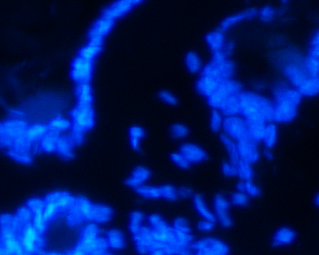
\includegraphics[width=4cm]{images/ADT_2_0.png} \caption{ภาพต้นฉบับ}
  \label{fig:img_original}
\end{subfigure}%
\begin{subfigure}{.45\textwidth}
  \centering
  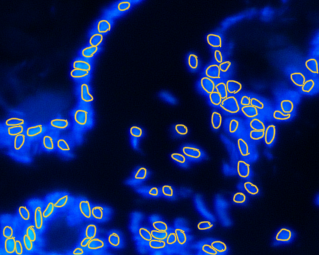
\includegraphics[width=4cm]{images/ADT_2_0_label.png} \caption{ภาพ label ตำแหน่งนิวเคลียสโดยนักพยาธิวิทยา}
  \label{fig:img_label}
\end{subfigure}
\caption{ภาพที่ใช้ในการพัฒนาแบบจำลอง}
\label{fig:img_train}
\end{figure}
\begin{figure}[!h]
    \centering
    \captionsetup{justification=centering}
    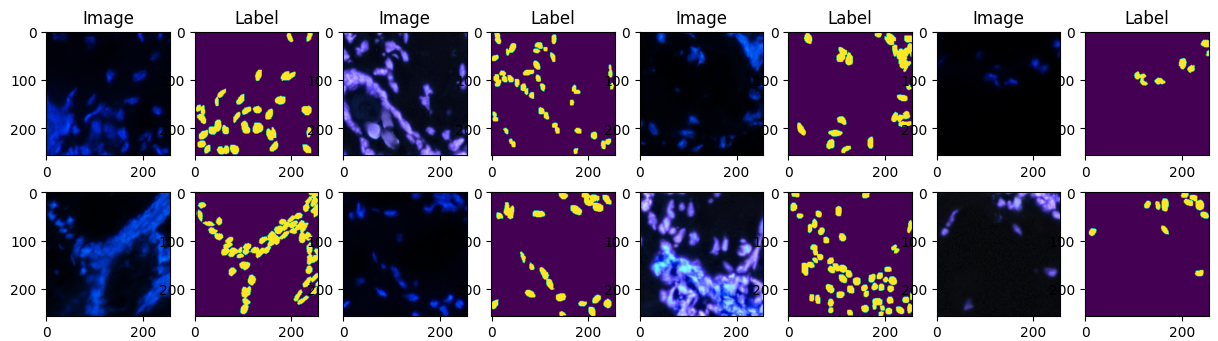
\includegraphics[scale=0.45]{images/data_aug_edit.png}
    \caption[รูปตัวอย่างจาก augment ]{ภาพผลลัพธ์จากกระบวนการ Augmentation}
    \label{fig:img_augment_example}
\end{figure}
\pagebreak
\item \textbf{Mask R-CNN} 
คณะผู้วิจัยได้ทำการทดลองกับแบบจำลอง Mask R-CNN มาใช้ฝึกกับชุดข้อมูลที่ใช้ในการพัฒนาแบบจำลองที่ได้กล่าวไว้ก่อนหน้านี้ โดยทำการปรับค่าพารามิเตอร์ ดังนี้ Backbone เท่ากับ Restnet101, Epochs เท่ากับ 100 ซึ่งจะเลือกเอาเฉพาะ epochs ที่ได้ค่าดีที่สุด และ Input size เท่ากับ 512 × 512 พิกเซล นอกจากนี้คณะผู้วิจัยทดลองปรับค่าพารามิเตอร์เพิ่มเพื่อให้ได้ค่า precision และ recall ที่สูงที่สุด โดยค่าของพารามิเตอร์ที่ทำให้ precision และ recall สูงที่สุดจะแสดงในตาราง \ref{tbl:maskrcnnpara} การทดลองนี้จะใช้ทั้งหมด 2 พารามิเตอร์คือ Non-maximum Suppression (NMS) และ ค่า Momentum โดยพารามิเตอร์ Non-maximum Suppression (NMS) ถูกปรับเพื่อให้การทำนายการตรวจหาตำแหน่งของนิวเคลียสดียิ่งขึ้น\cite{k_2019} โดยปรับจาก 0.3 เป็น 0.5 และปรับค่าพารามิเตอร์ momentum จาก 0.9 เป็น 0.3 ซึ่งการลดค่า momentum นั้นจะเป็นการลดความเร็วในการเรียนรู้ของแบบจำลองลง \cite{momentum} 

\begin{table}[!h]
\caption{ตารางการปรับพารามิเตอร์ของแบบจำลอง Mask R-CNN}\label{tbl:maskrcnnpara}
\begin{tabular}{>{\centering}p{0.2\textwidth}>{\centering}p{0.4\textwidth}>{\centering\arraybackslash}p{0.3\textwidth}}
\toprule
Model      & Parameter & Value\\ \midrule
  Mask R-CNN & Non-maximum Suppression (NMS) & 0.5  \\ 
 & momentum & 0.3  \\ \bottomrule
\end{tabular}
\end{table}
\item \textbf{YOLO} 
คณะผู้วิจัยใช้แบบจำลองจาก Glenn Joche \cite{yolo-repo} มาใช้ฝึกกับชุดข้อมูลที่ใช้ในการพัฒนาแบบจำลองที่ได้กล่าวไว้ก่อนหน้านี้ โดยทำการปรับค่าพารามิเตอร์ ดังนี้ Batch size เท่ากับ 32, Epochs เท่ากับ 100 ซึ่งจะเลือกเอาเฉพาะ epochs ที่ได้ค่าดีที่สุด และ Input size เท่ากับ 640x640 พิกเซล นอกจากนี้คณะผู้วิจัยทดลองปรับค่าพารามิเตอร์เพิ่มเพื่อให้ได้ค่า precision และ recall ที่สูงที่สุดโดยค่าของพารามิเตอร์ที่ทำให้ precision และ recall สูงที่สุดจะแสดงในตาราง \ref{tbl:YOLOpara} การทดลองนี้จะใช้ทั้งหมด 6 พารามิเตอร์ พารามิเตอร์ที่ 1 Dropout ซึ่งคือการสุ่มลด node ของแบบจำลองโดยจะใส่ค่าความน่าจะเป็นเพื่อลดความ Overfit ของแบบจำลอง \cite{Dropout2d} พารามิเตอร์ที่ 2 Leaky เพื่อเปลี่ยนค่าสัมประสิทธิ์ความชันในช่วงติดลบตั้งแต่ 0 ลงไปซึ่งการลดค่าสัมประสิทธิ์ความชันจะทำให้แบบจำลองลดความซับซ้อนลง โดยแบบจำลองเดิมจะมีค่า Default 0.3  \cite{LeakyReLU} พารามิเตอร์ที่ 3 Hardswish จะเป็นการเปิดใช้งานที่ใช้การคำนวณด้วยอะนาล็อกเชิงเส้นแบบแยกส่วน ซึ่งจะช่วยให้แบบจำลองคำนวนช้าลง \cite{Hardswish} พารามิเตอร์ที่ 4 การปรับค่า momentum โดยจากแบบจำลองเดิมจะมีค่าอยู่ที่ 0.937 ซึ่งการลดค่าของ momentum คือการลดความเร็วในการเรียนรู้ของแบบจำลองลง \cite{momentum} พารามิเตอร์ที่ 5 การปรับค่า scale image จากแบบจำลองเดิมจะตั้งค่าไว้ที่ 0.5 โดยการเพิ่มค่าให้เพิ่มขึ้นจะเพิ่มขนาดของภาพเพิ่มขึ้นก่อนเข้าแบบจำลอง และพารามิเตอร์ที่ 6 object loss การลดค่า object loss คือการลดค่า loss ในแต่ละพิกเซล โดยจากแบบจำลองเดิมตั้งค่าไว้ที่ 1.0\cite{scale} 

\begin{table}[!h]
\caption{ตารางการปรับพารามิเตอร์ของแบบจำลอง YOLO}\label{tbl:YOLOpara}
\begin{tabular}{>{\centering}p{0.2\textwidth}>{\centering}p{0.4\textwidth}>{\centering\arraybackslash}p{0.3\textwidth}}
\toprule
Model      & Parameter & Value\\ \midrule
 & Dropout & 0.1  \\ 
 & Leaky & 0.1  \\ 
 YOLO & momentum & 0.9  \\ 
 & scale image & 0.8    \\ 
 & object loss & 0.5   \\  \bottomrule
\end{tabular}
\end{table}
\pagebreak
\item \textbf{U-Net}

คณะผู้วิจัยได้แบ่งการทดลองออกเป็น 3 แบบจำลอง ประกอบด้วย U-Net คือ แบบจำลองตามโครงสร้างเดิมจากงานวิจัยของ Olaf Ronneberger และคณะ \cite{unet-model}, InceptionResNetV2 U-Net (IRNV2 U-Net) คือ แบบจำลองที่ใช้ส่วน Encoder ด้วย Pre-train weights ของ InceptionResNetV2 และคงส่วนของ Bottleneck และ Decoder ไว้เช่นเดิม และ Residual Attention U-Net (RA U-Net) ทั้ง 3 แบบจำลองคณะผู้วิจัยได้ทำการปรับค่าพารามิเตอร์ดังนี้ Batch size เท่ากับ 8, Epochs เท่ากับ 100 ซึ่งจะเลือกเอาเฉพาะ epochs ที่ได้ค่าดีที่สุด และ Input size 512x512 พิกเซล โดยตั้งค่า Earlystopper และใช้ Epochs ที่ให้ค่า Validation loss น้อยที่สุด ซึ่งคณะผู้วิจัยได้เลือกใช้ Adam และ Stochastic Gradient Descent (SGD) สำหรับ Optimizer ควบคู่กับ Binary Cross-Entropy (BCE) และใช้ Jaccard Coefficient ร่วมกับ Dice Coefficient สำหรับ Loss function สรุปได้ดังตารางที่ \ref{tab:unetconf}

\begin{table}[!h]
    \centering
    \caption{ตารางการปรับพารามิเตอร์ของแบบจำลอง U-Net}
    \label{tab:unetconf}
    \begin{tabular}{>{\centering}p{0.2\textwidth}>{\centering}p{0.4\textwidth}>{\centering\arraybackslash}p{0.3\textwidth}}
\toprule
Model  & Optimizer & Loss Function\\ \midrule
 U-Net & Adam  & BCE  \\
 &  & Dice+Jaccard  \\
 & SGD & BCE  \\ 
 &  & Dice+Jaccard  \\ 
IRNV2 U-Net & Adam & BCE  \\ 
 &  & Dice+Jaccard  \\
 & SGD & BCE  \\ 
 &  & Dice+Jaccard  \\ 
 RA U-Net & Adam & BCE  \\ 
 &  & Dice+Jaccard  \\
 & SGD & BCE  \\ 
 &  & Dice+Jaccard  \\  \bottomrule
    \end{tabular}
\end{table}

จากผลลัพธ์ของแบบจำลอง U-Net ทั้งหมดจะได้เป็นพื้นที่นิวเคลียสที่ไม่ได้แบ่งแยกกัน จึงจำเป็นต้องมีกระบวนการในการแบ่งนิวเคลียสที่ติดกันและนับจำนวนนิวเคลียส จากงานวิจัยของ Md Mostafa Sark และคณะ \cite{30}  ได้ใช้กระบวนการ Distance transform ควบคู่กับ Watershed เพื่อแบ่งนิวเคลียสที่ติดกันและ label นิวเคลียสออกจากกัน ทำให้ได้ผลลัพธ์เป็นตำแหน่งและจำนวนของแต่ละนิวเคลียส โดยตัวอย่างผลลัพธ์แสดงดังรูปภาพที่ \ref{fig:unet-pred}
\begin{figure}[!h]
    \centering
    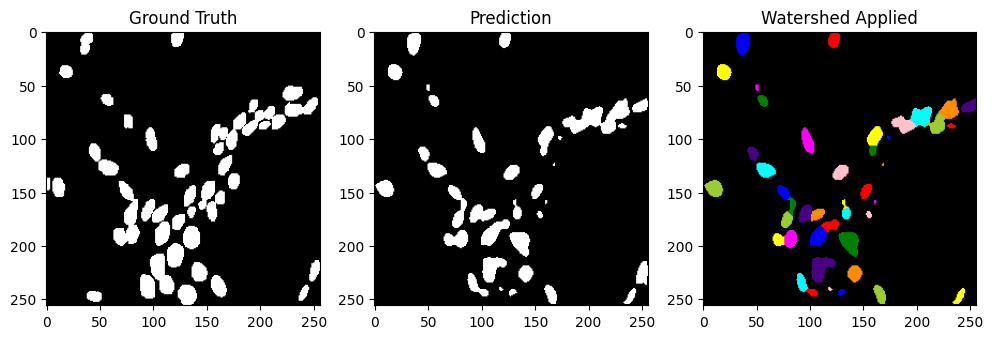
\includegraphics[scale=0.5]{images/unet_pred.png}
    \captionsetup{justification=centering}
    \caption{ค่าพื้นที่จริงของนิวเคลียส (ซ้าย), ผลลัพธ์จากแบบจำลอง U-Net (กลาง) และ ผลลัพธ์จาก Watershed (ขวา)}
    \label{fig:unet-pred}
\end{figure}

\end{itemize}
\pagebreak
\subsubsection{การประมวลผลภาพ (Image Processing)}
จากการศึกษางานวิจัยที่เกี่ยวข้องในตารางที่ \ref{tbl:image processing} คณะผู้วิจัยสรุปขั้นตอนโดยแบ่งออกเป็น 3 ขั้นตอนหลัก ประกอบด้วย การแยกวัตถุออกจากพื้นหลัง (Thresholding), การแบ่งนิวเคลียสที่ซ้อนทับกัน (Split touching Nucleus) และ การนับจำนวนนิวเคลียส (Nucleus counting) ตัวอย่างผลลัพธ์จากขั้นตอนแสดงดังรูปภาพที่ \ref{fig:imks-process}
\begin{figure}[!h]
    \centering
    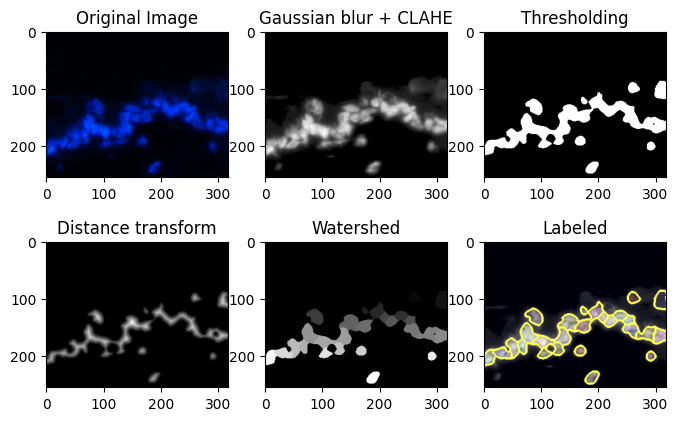
\includegraphics[scale=0.6]{images/imks_process.png}
    \caption[imks-process]{ผลลัพธ์จากการใช้กระบวนการของ Image Processing ในแต่ละขั้นตอน}
    \label{fig:imks-process}
\end{figure}
\begin{itemize}[listparindent=\parindent]
% \setlength{\itemindent}{.3in}
\item \textbf{Preprocessing} 
กระบวนการก่อนการประมวลผลภาพนั้นประกอบด้วยการแปลงรูปภาพสีให้อยู่ในช่วงสีเทา (RGB to Grayscale) แล้วทำการลดสัญญาณรบกวนด้วย Gaussian Blur จากนั้นปรับปรุงค่า Contrast ของรูปด้วย Contrast Limited Adaptive Histogram Equalization เพื่อดึงความสว่างของนิวเคลียสให้ชัดเจนยิ่งขึ้น

\item \textbf{Thresholding} 
เราใช้การแยกวัตถุออกจากพื้นหลังด้วย Short range \& Long range Local Average Threshold \cite{28} เนื่องจากรูป Datasets ประกอบด้วยช่วงความสว่างแสงที่แตกต่างกัน โดย Short range Thresholding จะทำ Thresholding ที่ค่าต่ำ ซึ่งจะได้ผลลัพธ์เป็นขอบของนิวเคลียส แต่อาจจะมีวัตถุชิ้นเล็กๆที่ไม่ใช่นิวเคลียสถูก Thresholding มาด้วย ดังนั้นการทำ Long range Thresholding จะทำ Thresholding ที่ค่าสูงกว่า เมื่อนำค่าทั้งสองมารวมกันจะทำให้สามารถลบช่วงสว่างที่ไม่ใช่นิวเคลียสออกไปได้ เหลือเพียงขอบของนิวเคลียสที่สนใจ

\item \textbf{Split touching Nucleus} 
ซึ่งทั้งงานวิจัยของ Wanjun Zhang \cite{28} และ Sonal Kothari \cite{30} ได้ใช้ขั้นตอนที่คล้ายกันนั่นคือการหา Concave point \cite{28} ด้วย Harris Corner Detection และ Notch detection \cite{30} เพื่อใช้ในการระบุจุดที่เป็นมุมที่เกิดจากซ้อนทับกัน ซึ่งสามารถนำไปสู่กระบวนการ Ellipse fitting เพื่อทำการวงขอบนิวเคลียส และในส่วนของงานวิจัยของ Sven P. Voigt \cite{32} ได้ใช้กระบวนการที่คล้ายกับงานวิจัยที่กล่าวมาก่อนหน้านี้และเพิ่มกระบวนการ Distance Transform เพื่อนำไปใช้ Watershed ในการแบ่งส่วนนิวเคลียสที่ทับซ้อนกัน ซึ่งคณะผู้วิจัยได้ใช้วิธีของ Sven P. Voigt \cite{32} ในขั้นตอนนี้ ซึ่งผลลัพธ์ของ Watershed คือ Label ของแต่ละนิวเคลียส

\item \textbf{Nucleus counting} 
จากงานวิจัยของ Sven P. Voigt \cite{32} ได้พัฒนาขั้นตอนของตัวเองจาก scikit-image โดยการนับจำนวน Label ซึ่งจะได้ผลลัพธ์จำนวนนิวเคลียสจากขั้นตอนก่อนหน้าและยังคำนวนพื้นที่ของแต่ละนิวเคลียสที่นับได้จากการคำนวนพื้นที่ของแต่ละ Label ซึ่งคณะผู้วิจัยได้ใช้วิธีนี้สำหรับขั้นตอนนี้
\end{itemize}
\pagebreak
\subsection{การประเมินผลแบบจำลอง (Evaluation plans)}
\subsubsection{ประเภทของผลลัพธ์จากการเรียนรู้เชิงลึก (Deep Learning) และ การประมวลผลภาพ (Image Processing)}
ในกระบวนการวัดผลของทั้งการเรียนรู้เชิงลึก (Deep Learning) และ การประมวลผลภาพ (Image Processing) จะนำผลลัพธ์ที่ได้จากทั้ง 2 กระบวนการ มานับจำนวนนิวเคลียส โดยผลลัพธ์ที่ได้นั้นประกอบด้วย
\begin{itemize}
% \setlength{\itemindent}{.3in}
    \item \textbf{Ground Truth Number (GT)} หรือ ค่าที่ได้จากการ label ด้วยนักพยาธิวิทยา
    \item \textbf{True Positive (TP)} หรือ ค่าที่ได้จากการทำนายว่า พื้นที่นิวเคลียสนั้นได้คำตอบเป็นพื้นที่นิวเคลียส
    \item \textbf{False Positive (FP)} หรือ ค่าที่ได้จากการทำนายว่า พื้นหลังนั้นได้คำตอบเป็นพื้นที่นิวเคลียส
    \item \textbf{Flase Negative (FN)} หรือ ค่าที่ได้จากการทำนายว่า พื้นที่นิวเคลียสนั้นได้คำตอบเป็นพื้นหลัง
%    \item \textbf{Predict Combined (PC)} หรือ ค่าที่ได้จากการทำนายว่า พื้นที่นิวเคลียส 2 นิวเคลียสหรือมากกว่านั้นที่อยู่ติดกันได้คำตอบเป็นพื้นที่นิวเคลียสเดียว
%    \item \textbf{Object Combined (OC)} หรือ จำนวนนิวเคลียสของ Ground Truth Number ที่ถูกรวมในเงื่อนไขของ Predict Combined
    \item \textbf{Estimate Number (EN)} หรือ ค่าผลลัพธ์จำนวนนิวเคลียสทั้งหมดที่ได้มาจากการทำนาย
\end{itemize}
\subsubsection{วิธีการวัดผลที่นำมาใช้}
หลังจากที่ได้ผลลัพธ์ในรูปแบบข้างต้นจึงสามารถเลือกวิธีการวัดผลที่เหมาะสมได้ ซึ่งวิธีการวัดผลที่เราเลือกใช้จะประกอบด้วย
\begin{itemize}
% \setlength{\itemindent}{.3in}
\item \textbf{Precision} หรือ ค่าความแม่นยำของตำแหน่งพื้นที่นิวเคลียสจริงเทียบกับผลการทำนายตำแหน่งพื้นที่นิวเคลียสทั้งหมด เมื่อ Precision เท่ากับ 1 หมายความว่าความแม่นยำของการทำนายสูงที่สุด หรือ ผลลัพธ์มีค่า FP เท่ากับ 0 และเมื่อ Precision เท่ากับ 0 หมายความว่าความแม่นยำของการทำนายต่ำที่สุด หรือ ผลลัพธ์มีค่า TP เท่ากับ 0 โดยค่า Precision สามารถคำนวนได้ดังสมการ \ref{Eq:Precision}
    \begin{equation}
        Precision = \frac{TP}{TP + FP} \label{Eq:Precision}
    \end{equation}
    where:  $0 \leq Precision \leq 1$
    
\item \textbf{Recall} หรือ ค่าความครอบคลุมของตำแหน่งพื้นที่นิวเคลียสจริงเทียบกับผลการทำนายตำแหน่งพื้นที่ทั้งหมด เมื่อ Recall เท่ากับ 1 หมายความว่าความครอบคลุมของการทำนายสูงที่สุด หรือ ผลลัพธ์มีค่า FN เท่ากับ 0 และเมื่อ Recall เท่ากับ 0 หมายความว่าความครอบคลุมของการทำนายต่ำที่สุด หรือ ผลลัพธ์มีค่า TP เท่ากับ 0 โดยค่า Recall สามารถคำนวนได้ดังสมการ \ref{Eq:Recall}
    \begin{equation}
        Recall = \frac{TP}{TP + FN} \label{Eq:Recall}
    \end{equation}
    where:  $0 \leq Recall \leq 1$
    
\item \textbf{F1 Score} หรือ ค่าเฉลี่ยฮาร์โมนิคของ Precision และ Recall เมื่อ F1 Score เท่ากับ 1 หมายความว่า Precision และ Recall เท่ากับ 1 ทั้งคู่ และเมื่อ เมื่อ F1 Score เข้าใกล้ 0 หมายความว่า Precision และ Recall เข้าใกล้ 0 ทั้งคู่ ในกรณีที่ Precision และ Recall เท่ากับ 0 จะไม่สามารถคำนวนค่า F1 Score ได้ ซึ่งอนุมาณได้ว่าแบบจำลองนั้นไม่มีความสามารถในการทำนายเลย โดยค่า F1 Score สามารถคำนวนได้ดังสมการ \ref{Eq:F1}
    \begin{equation}
        F1 = \frac{2 \times Precision \times Recall}{Precision + Recall} \label{Eq:F1}
    \end{equation}
    where:  $0 < F1 \leq 1$  \\
    and: $Precision, Recall \neq 0$
    
\item \textbf{Estimate Number ratio (ENr)} หรือ อัตราส่วนระหว่าง EN เทียบกับ GT เมื่อ Estimate Number ratio เท่ากับ 1 หมายความว่าแบบจำลองทำนายผลลัพธ์ได้คำตอบเท่ากับค่าที่ได้จากการ label ด้วยนักพยาธิวิทยา ซึ่งอนุมาณว่าได้ผลลัพธ์จำนวนนิวเคลียสถูกต้อง, เมื่อ Estimate Number ratio มากกว่า 1 หมายความว่าแบบจำลองทำนายผลลัพธ์ได้คำตอบมากกว่าค่าที่ได้จากการ label ด้วยนักพยาธิวิทยา และเมื่อ Estimate Number ratio น้อยกว่า 1 หมายความว่าแบบจำลองทำนายผลลัพธ์ได้คำตอบน้อยกว่าค่าที่ได้จากการ label ด้วยนักพยาธิวิทยา โดยค่า Estimate Number ratio สามารถคำนวนได้ดังสมการ \ref{Eq:ENR}
    \begin{equation}
        ENr = \frac{EN}{GT} \label{Eq:ENR}
    \end{equation}
    where:  $0 \leq ENr \leq \infty$
    
\item \textbf{Dice Similarity Coefficient (DSC)} เป็นวิธีการวัดผลที่ใช้ในการวัดความเหมือนกันระหว่างตำแหน่งนิวเคลียสที่ได้จากนักพยาธิวิทยาและผลลัพธ์จากแบบจำลอง เป็นวิธีวัดผลที่ได้รับความนิยมในด้านการวิเคราะห์ภาพทางการแพทย์ \cite{DSC} เมื่อ DSC เท่ากับ 1 หมายความว่า พื้นที่ทำนายซ้อนทับกับพื้นที่จริงพอดี หรืออนุมาณได้ว่า แบบจำลองทำนายผลลัพธ์ได้ตำแหน่งถูกต้องทั้งหมด และเมื่อ DSC เท่ากับ 0 หมายความว่า พื้นที่ทำนายไม่มีการซ้อนทับกับพื้นที่จริงใดๆ หรืออนุมาณได้ว่า แบบจำลองไม่สามารถทำนายผลลัพธ์ได้ตำแหน่งที่ถูกต้องเลย สามารถคำนวนได้ดังสมการ \ref{Eq:DSC}
    \begin{equation}
        DSC = \frac{2 |A \cap B|}{|A| + |B|} \label{Eq:DSC}
    \end{equation}
    where: $0 \leq DSC \leq 1$ \\
    and: $A =$ Area of Ground Truth, $B =$ Area of Predicted

% \item \textbf{Intersection over Union (IoU)} เป็นวิธีการวัดผลที่ใช้ในการวัดการซ้อนทับกันระหว่างตำแหน่งนิวเคลียสที่ได้จากนักพญาธิวิทยาและผลลัพธ์จากแบบจำลอง สามารถคำนวนได้ดังสมการ \ref{Eq:IoU}
%     \begin{equation}
%         IoU = \frac{|A \cap B|}{|A\cup B|} \label{Eq:IoU}
%     \end{equation}
%     where:  $A =$ Ground Truth, $B =$ Predicted
    
\end{itemize}
\section{การพัฒนาเว็บแอปพลิเคชัน}
\subsection{แผนภาพสถาปัตยกรรมของระบบ}
คณะผู้วิจัยได้พัฒนาเว็บแอปพลิเคชันบนพื้นฐานของภาษา Python ด้วย Framework ต่าง ๆ เข้าด้วยกัน ซึ่งเว็บแอปพลิเคชันสามารถแปลงให้อยู่ในรูปแบบของ Containerization ได้และ deploy ได้บน Web Serverless services ซึ่งคณะผู้วิจัยได้แยกการพัฒนาออกเป็นสองส่วน ประกอบด้วย การพัฒนาแบบจําลองในการนับจํานวนนิวเคลียสที่กล่าวในหัวข้อก่อนหน้า และ การพัฒนาเว็บแอปพลิเคชัน แล้วนำอัลกอริทึมที่ดีที่สุดเป็นเบื้องหลังของการนับจำนวนนิวเคลียส จากนั้นแปลง source code ให้อยู่ในรูปแบบของ Docker Image เพื่อนำไป deploy บน Firebase ซี่งทำหน้าที่เป็น Web hosting ทำงานร่วมกับ Cloud Run ซี่งทำหน้าที่เป็น Web Serverless services โดยโครงสร้างของเว็บแอปพลิเคชันแสดงดังรูปที่ \ref{fig:Webapparch}
\begin{figure}[!h]
    \centering
    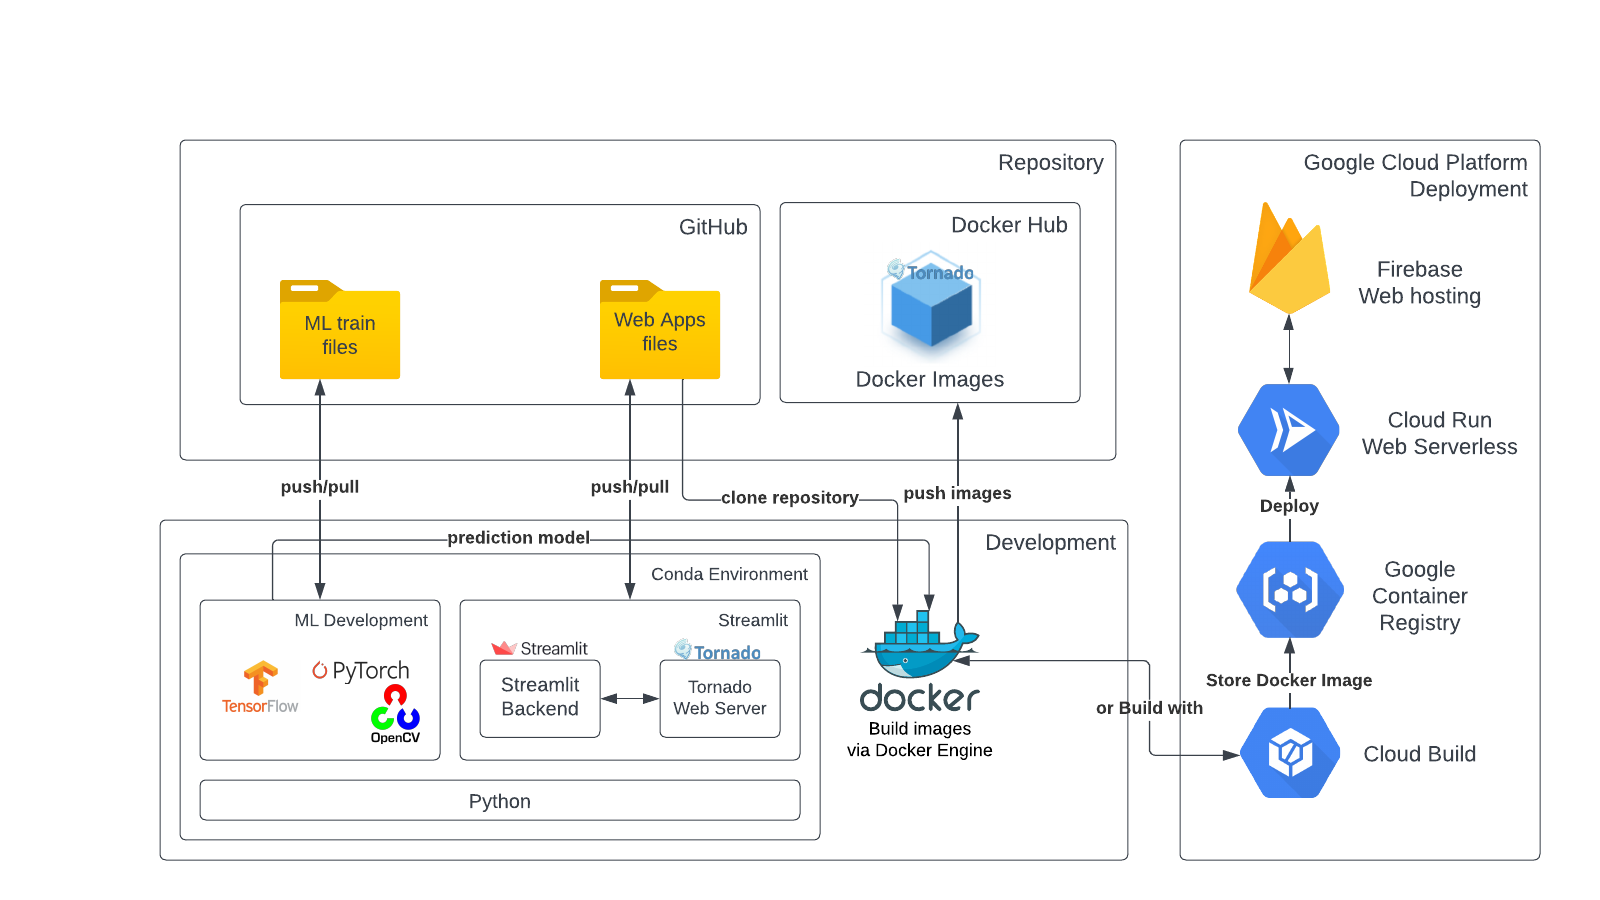
\includegraphics[width=11cm]{images/Webappstr.png}
    \caption{โครงสร้างของเว็บแอปพลิเคชัน}
    \label{fig:Webapparch}
\end{figure}
\subsection{ส่วนต่อประสานกับผู้ใช้ (User Interface Design)}
ใช้ Streamlit และภาษา Python ในการออกแบบสร้างเว็บแอปพลิเคชัน โดยหน้าเว็บแอปพลิเคชันจะมีส่วนต่าง ๆ ประกอบด้วยสองส่วน 

\textbf{ส่วนหน้าแรก}
ส่วนหน้าแรกของเว็บแอปพลิเคชัน จะมีรายละเอียดโดยย่อ ดังแสดงในรูปที่~\ref{fig:web_home1} และขั้นตอนใช้งานของเว็บแอปพลิเคชัน ดังแสดงในรูปที่~\ref{fig:web_home2}
\begin{figure}[!h]
\centering
    \begin{subfigure}[b]{0.42\textwidth}
      \centering
        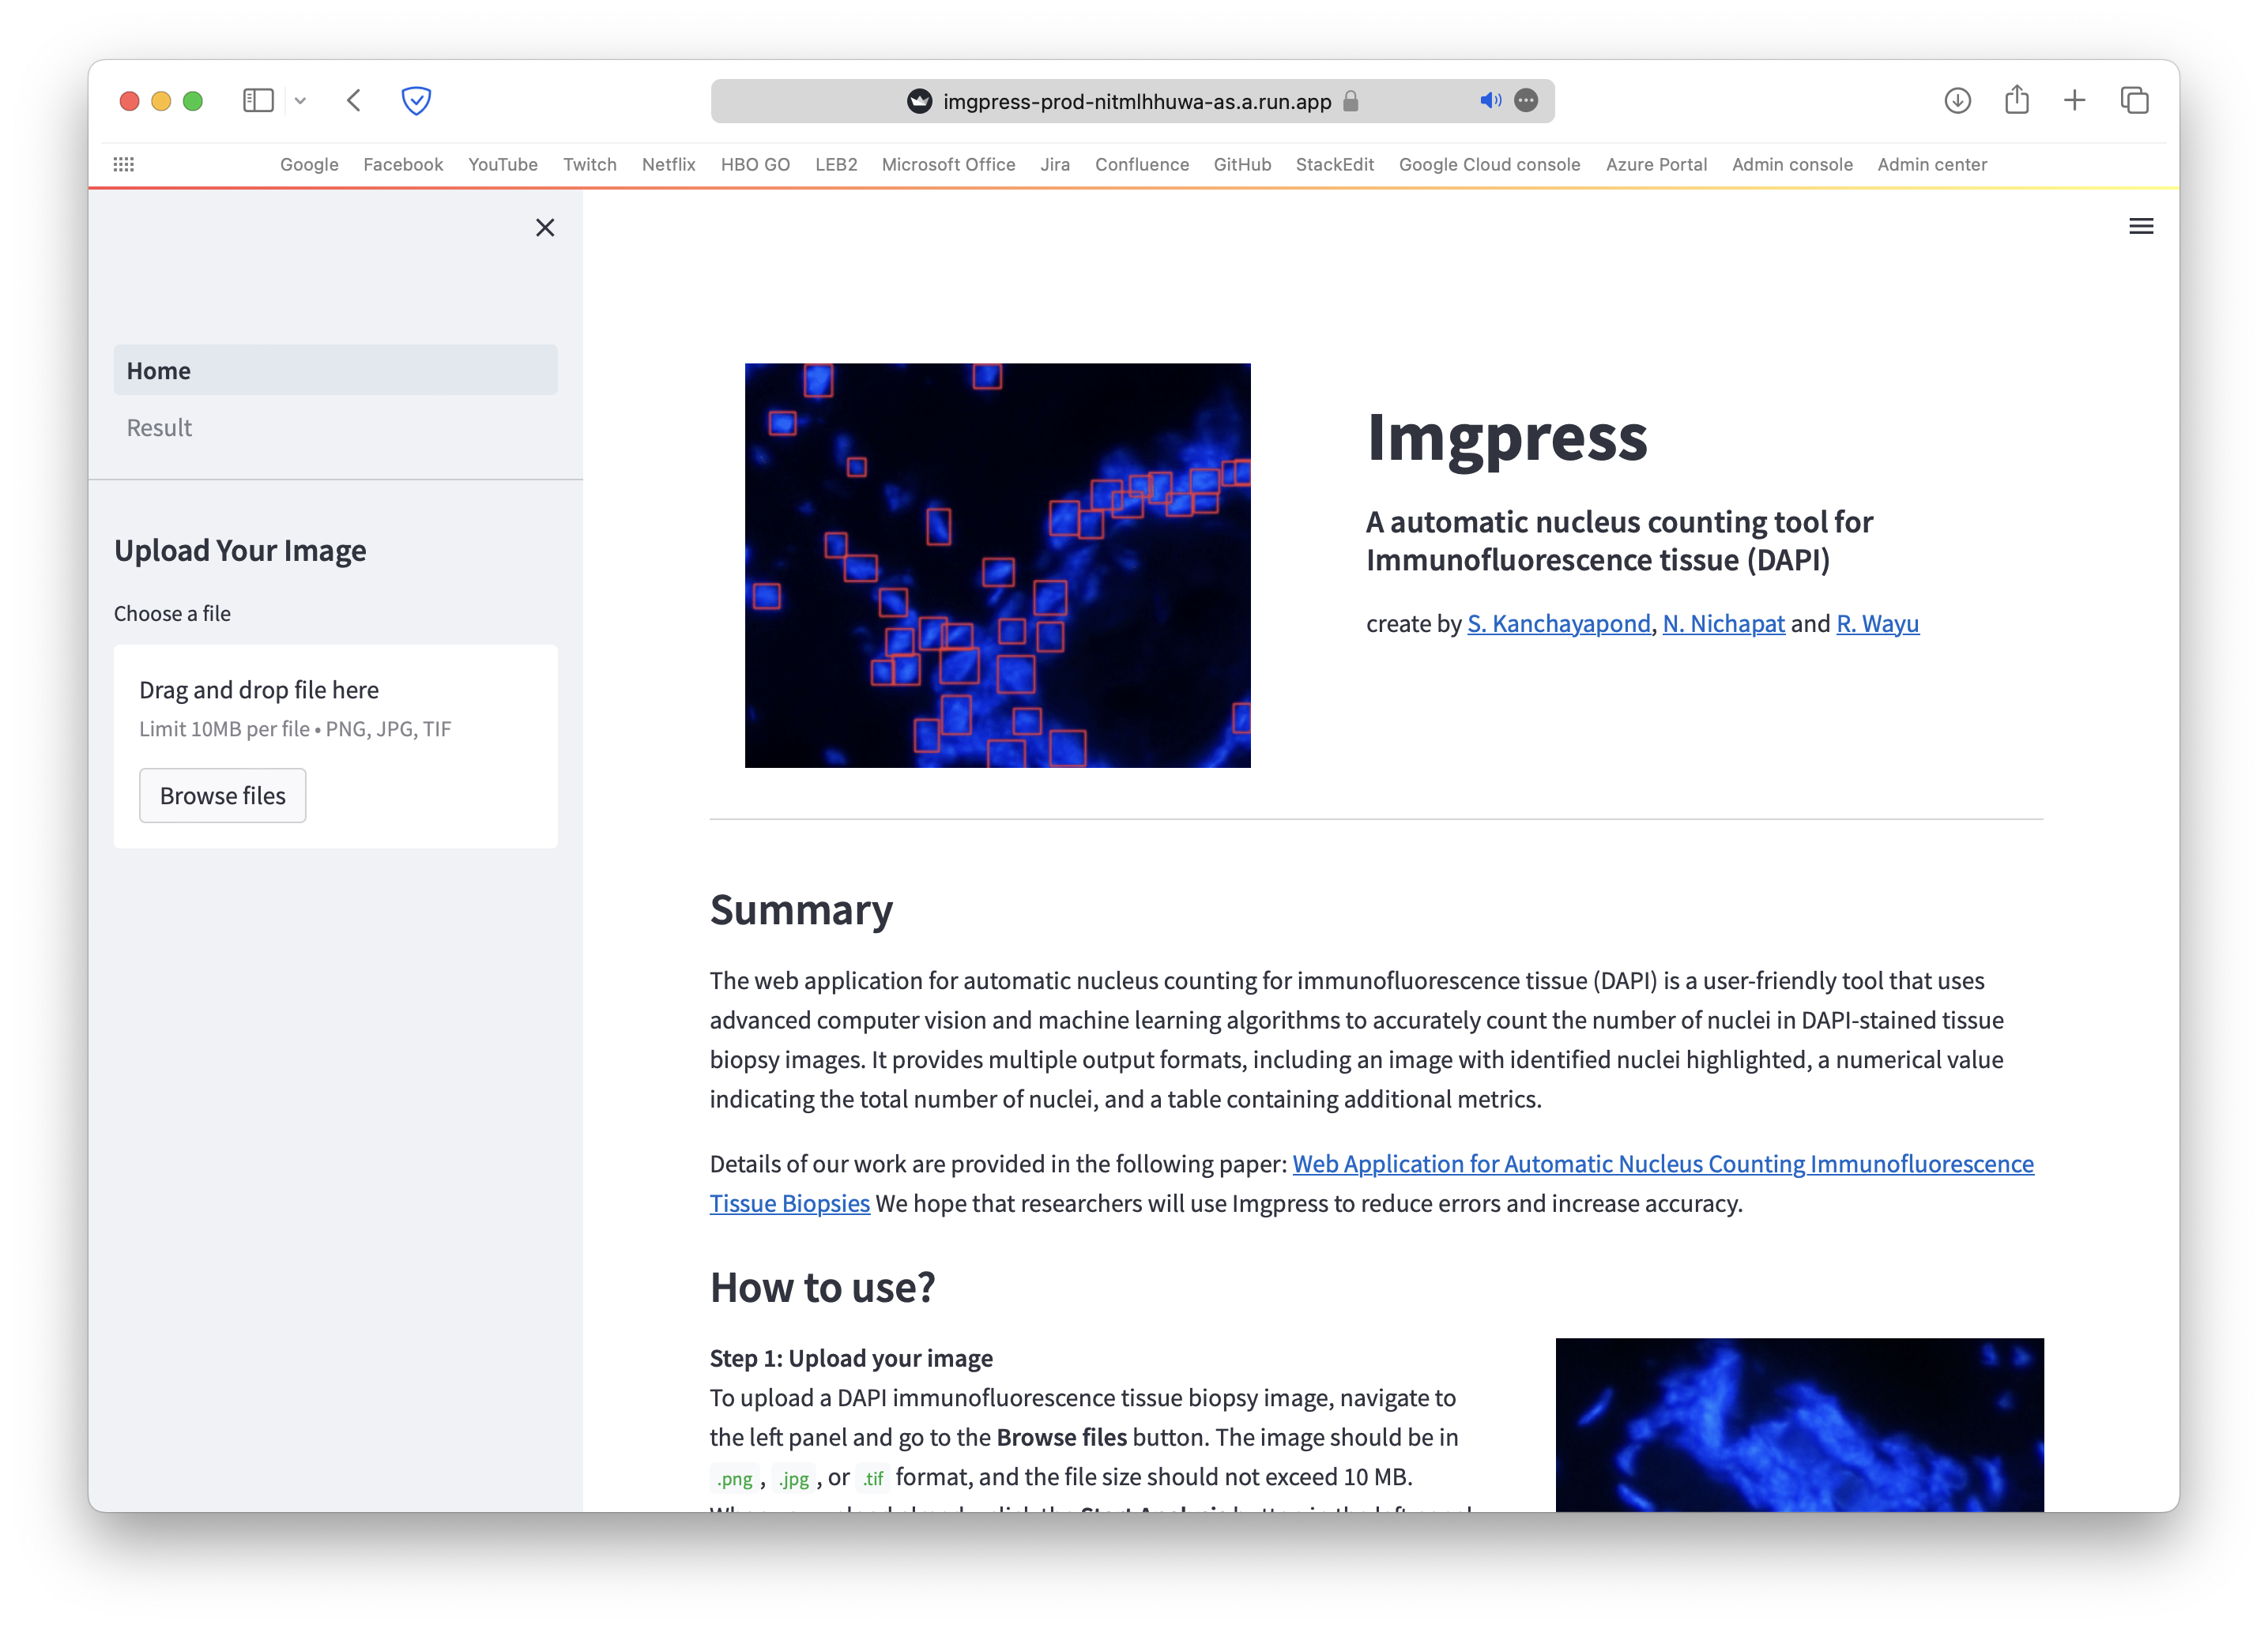
\includegraphics[width=\textwidth]{images/homepage.png}
        % \captionsetup{justification=centering}
        \caption{ส่วนหน้าแรกของเว็บแอปพลิเคชัน}\label{fig:web_home1}
    \end{subfigure}
    \begin{subfigure}[b]{0.42\textwidth}
        \centering
        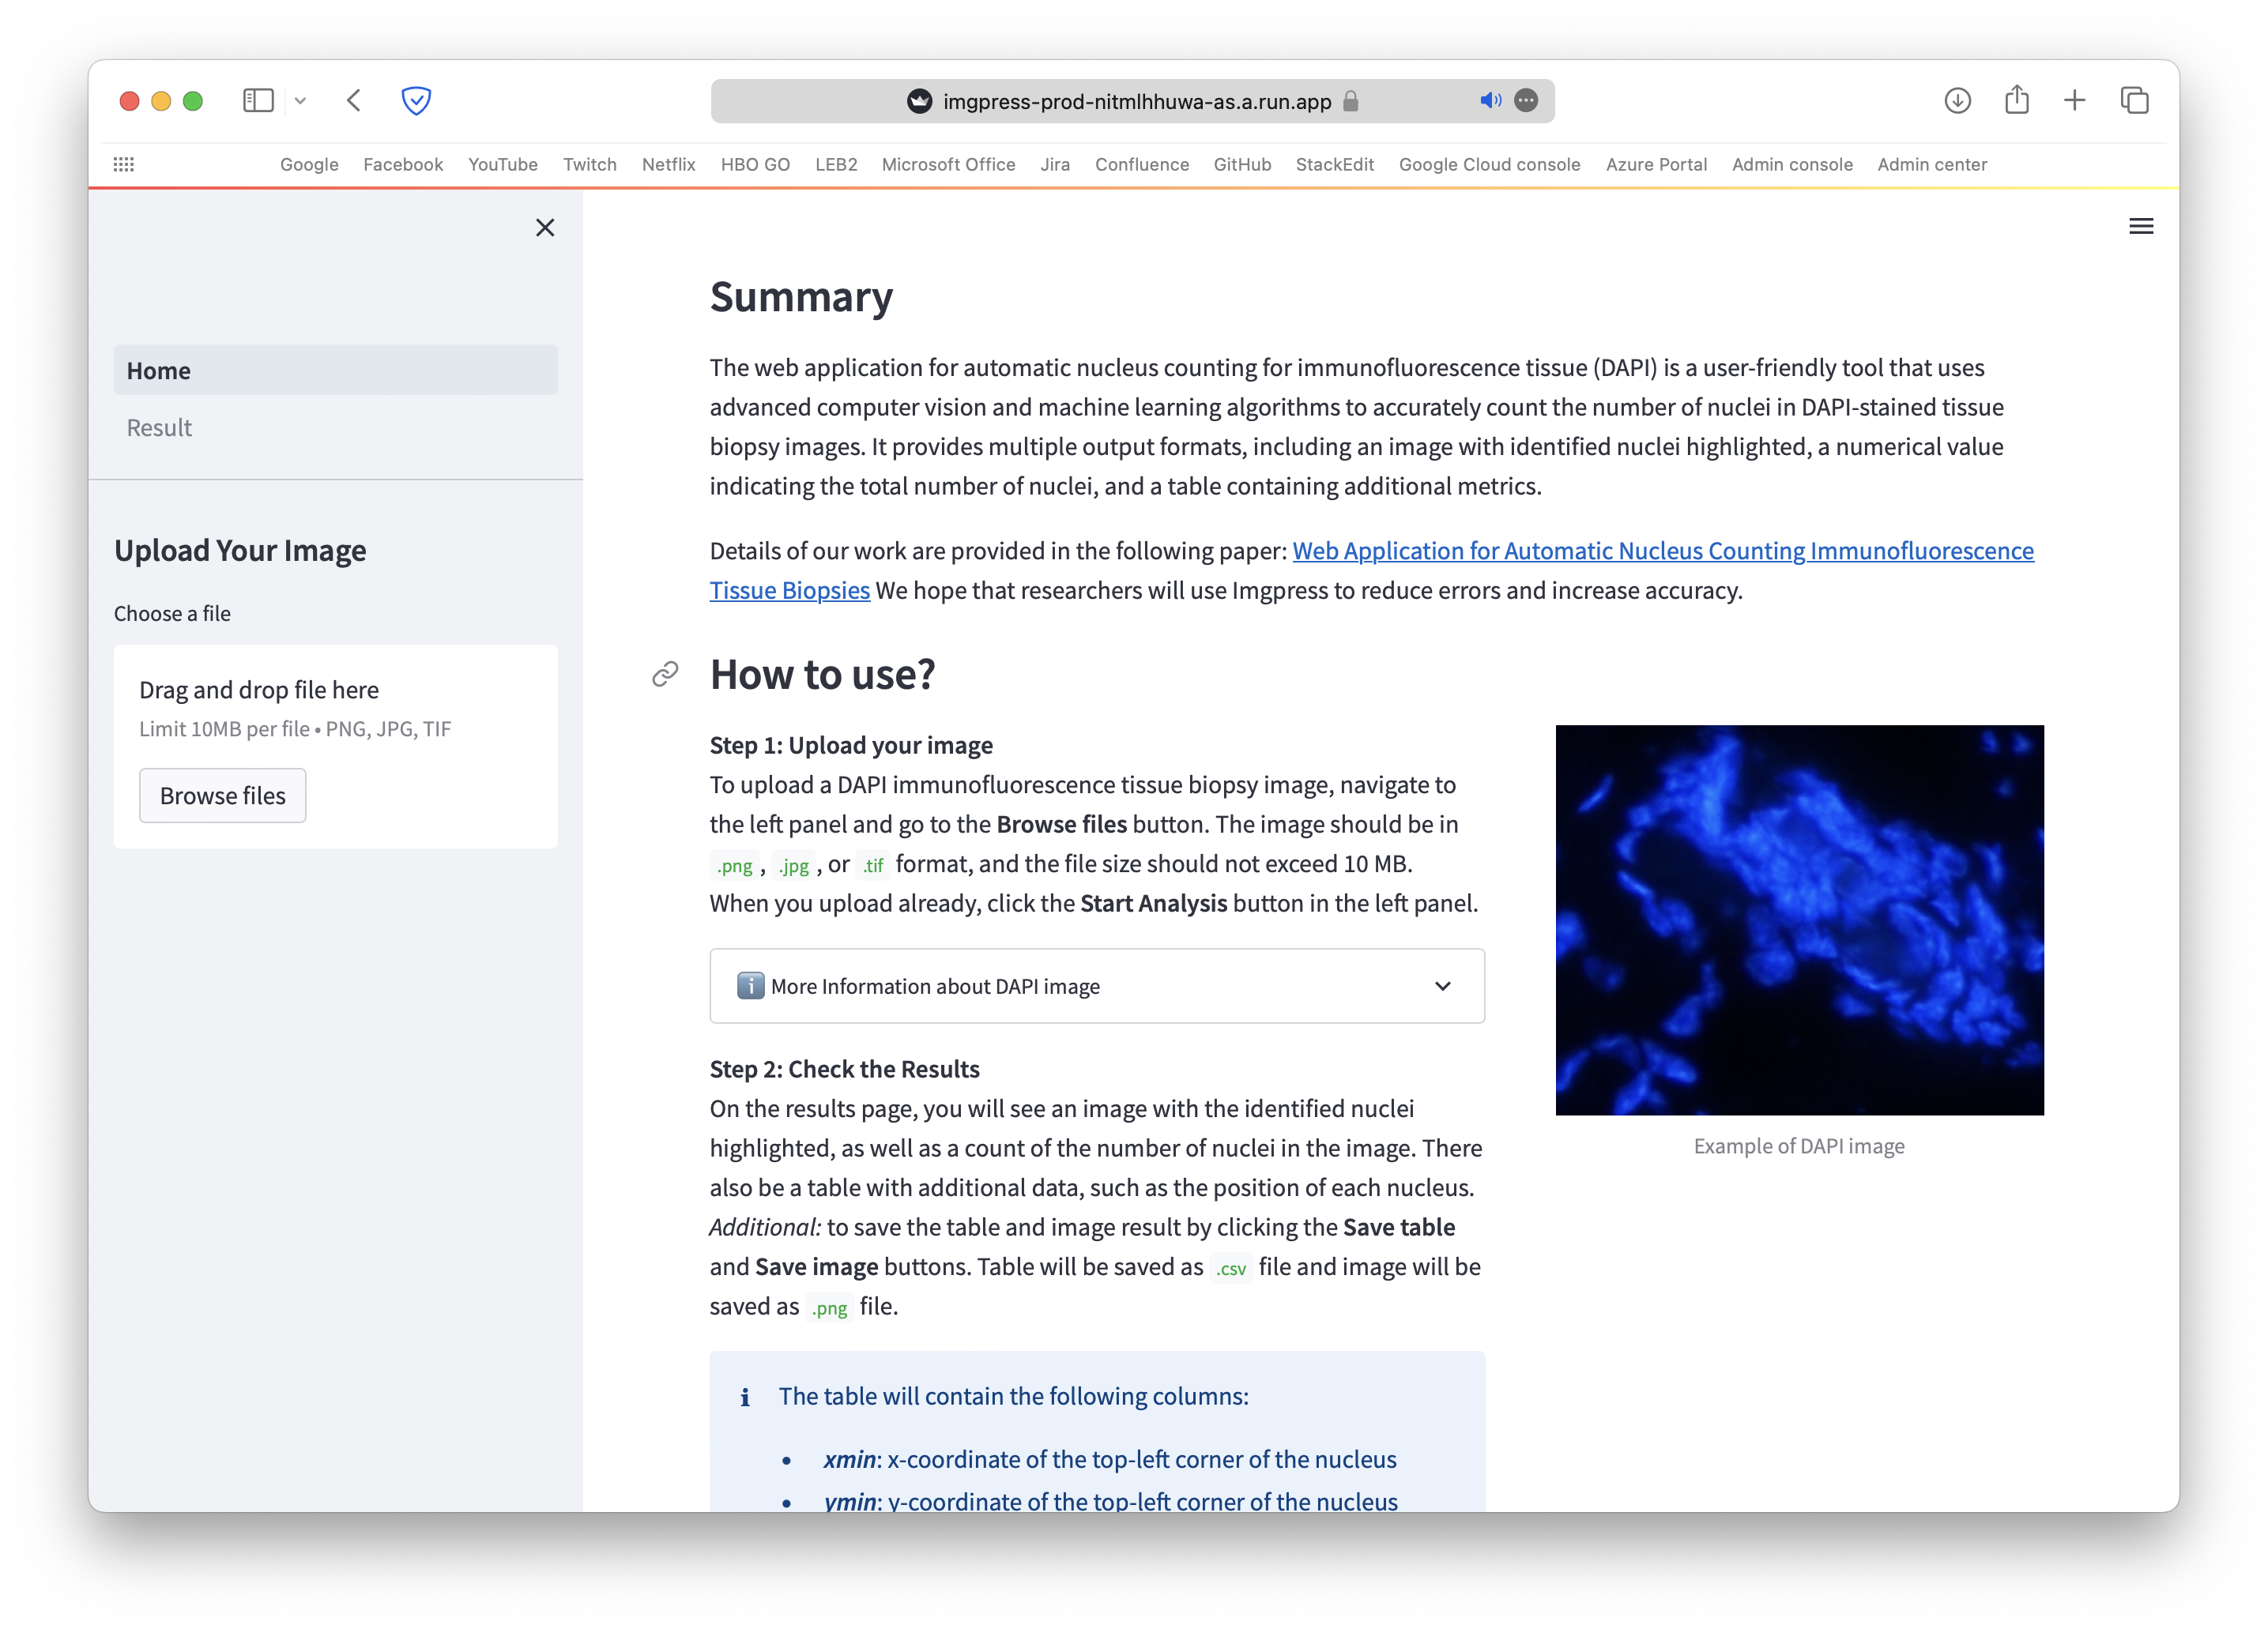
\includegraphics[width=\textwidth]{images/usage.png}
        % \captionsetup{justification=centering}
        \caption{ขั้นตอนใช้งานของเว็บแอปพลิเคชัน}\label{fig:web_home2}
    \end{subfigure}
    \caption{ส่วนหน้าแรกของเว็บแอปพลิเคชัน}
    \label{fig:uploadweb}
\end{figure}
\pagebreak

\textbf{ส่วนอัปโหลดรูป}

ส่วนอัปโหลดรูปจะมีคำอธิบายเกี่ยวกับรูปที่จะสามารถอัปโหลดและรูปตัวอย่างบริเวณด้านล่างของปุ่ม Browse files ดังแสดงในรูปหน้าแรกของเว็บแอปพลิเคชันรูปที่~\ref{fig:web_home1} ซึ่งปุ่ม Browse files จะใช้ในการอัปโหลดรูปที่ต้องการทราบตำแหน่งของนิวเคลียสเมื่อกดปุ่มแล้วจะขึ้นโฟลเดอร์เพื่อให้เลือกรูปที่จะอัปโหลดดังแสดงในรูปที่~\ref{fig:web_upload1}  และเมื่ออัพโหลดรูปที่ต้องการแล้วรูปที่อัปโหลดจะแสดงที่บริเวณทางด้านล่างของปุ่ม Browse files ดังแสดงในรูปที่~\ref{fig:web_upload2} 
\begin{figure}[!h]
\centering
    \begin{subfigure}[b]{0.42\textwidth}
      \centering
        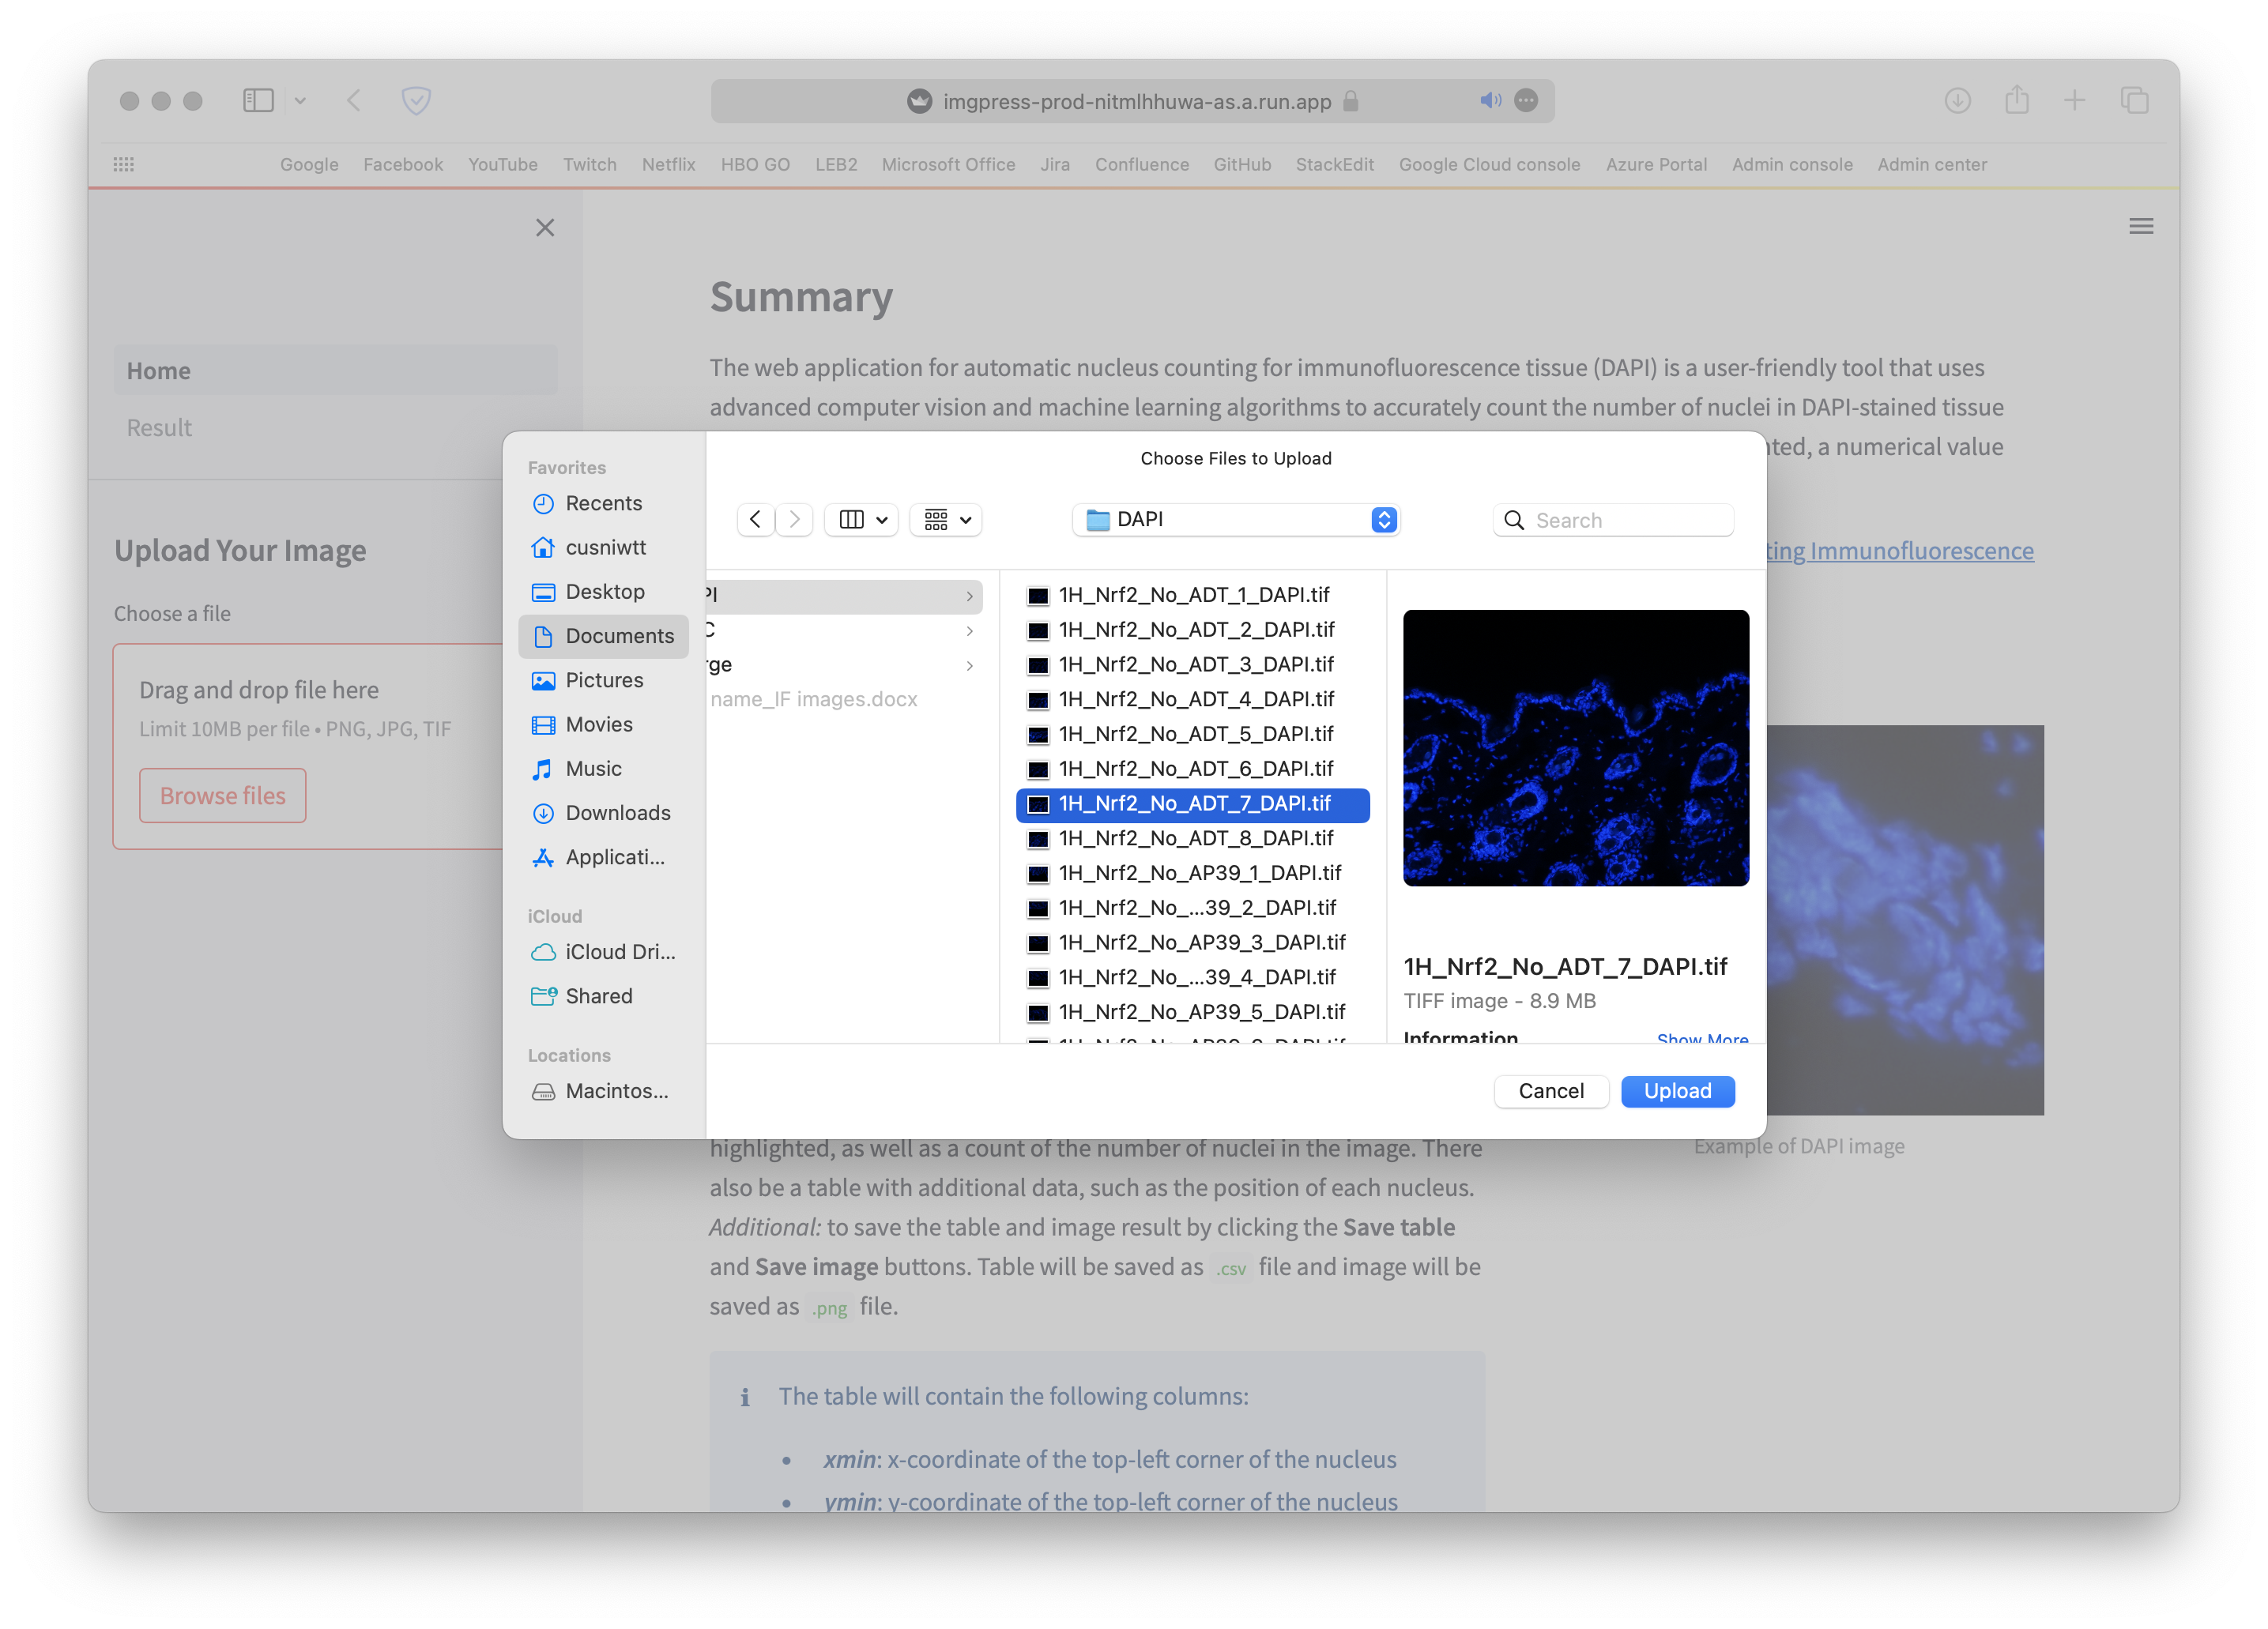
\includegraphics[width=\textwidth]{images/upload.png}
        % \captionsetup{justification=centering}
        \caption{หลังจากกดปุ่ม Browse files จะให้้เลือกไฟล์ภาพจาก}\label{fig:web_upload1}
    \end{subfigure}
    \begin{subfigure}[b]{0.42\textwidth}
        \centering
        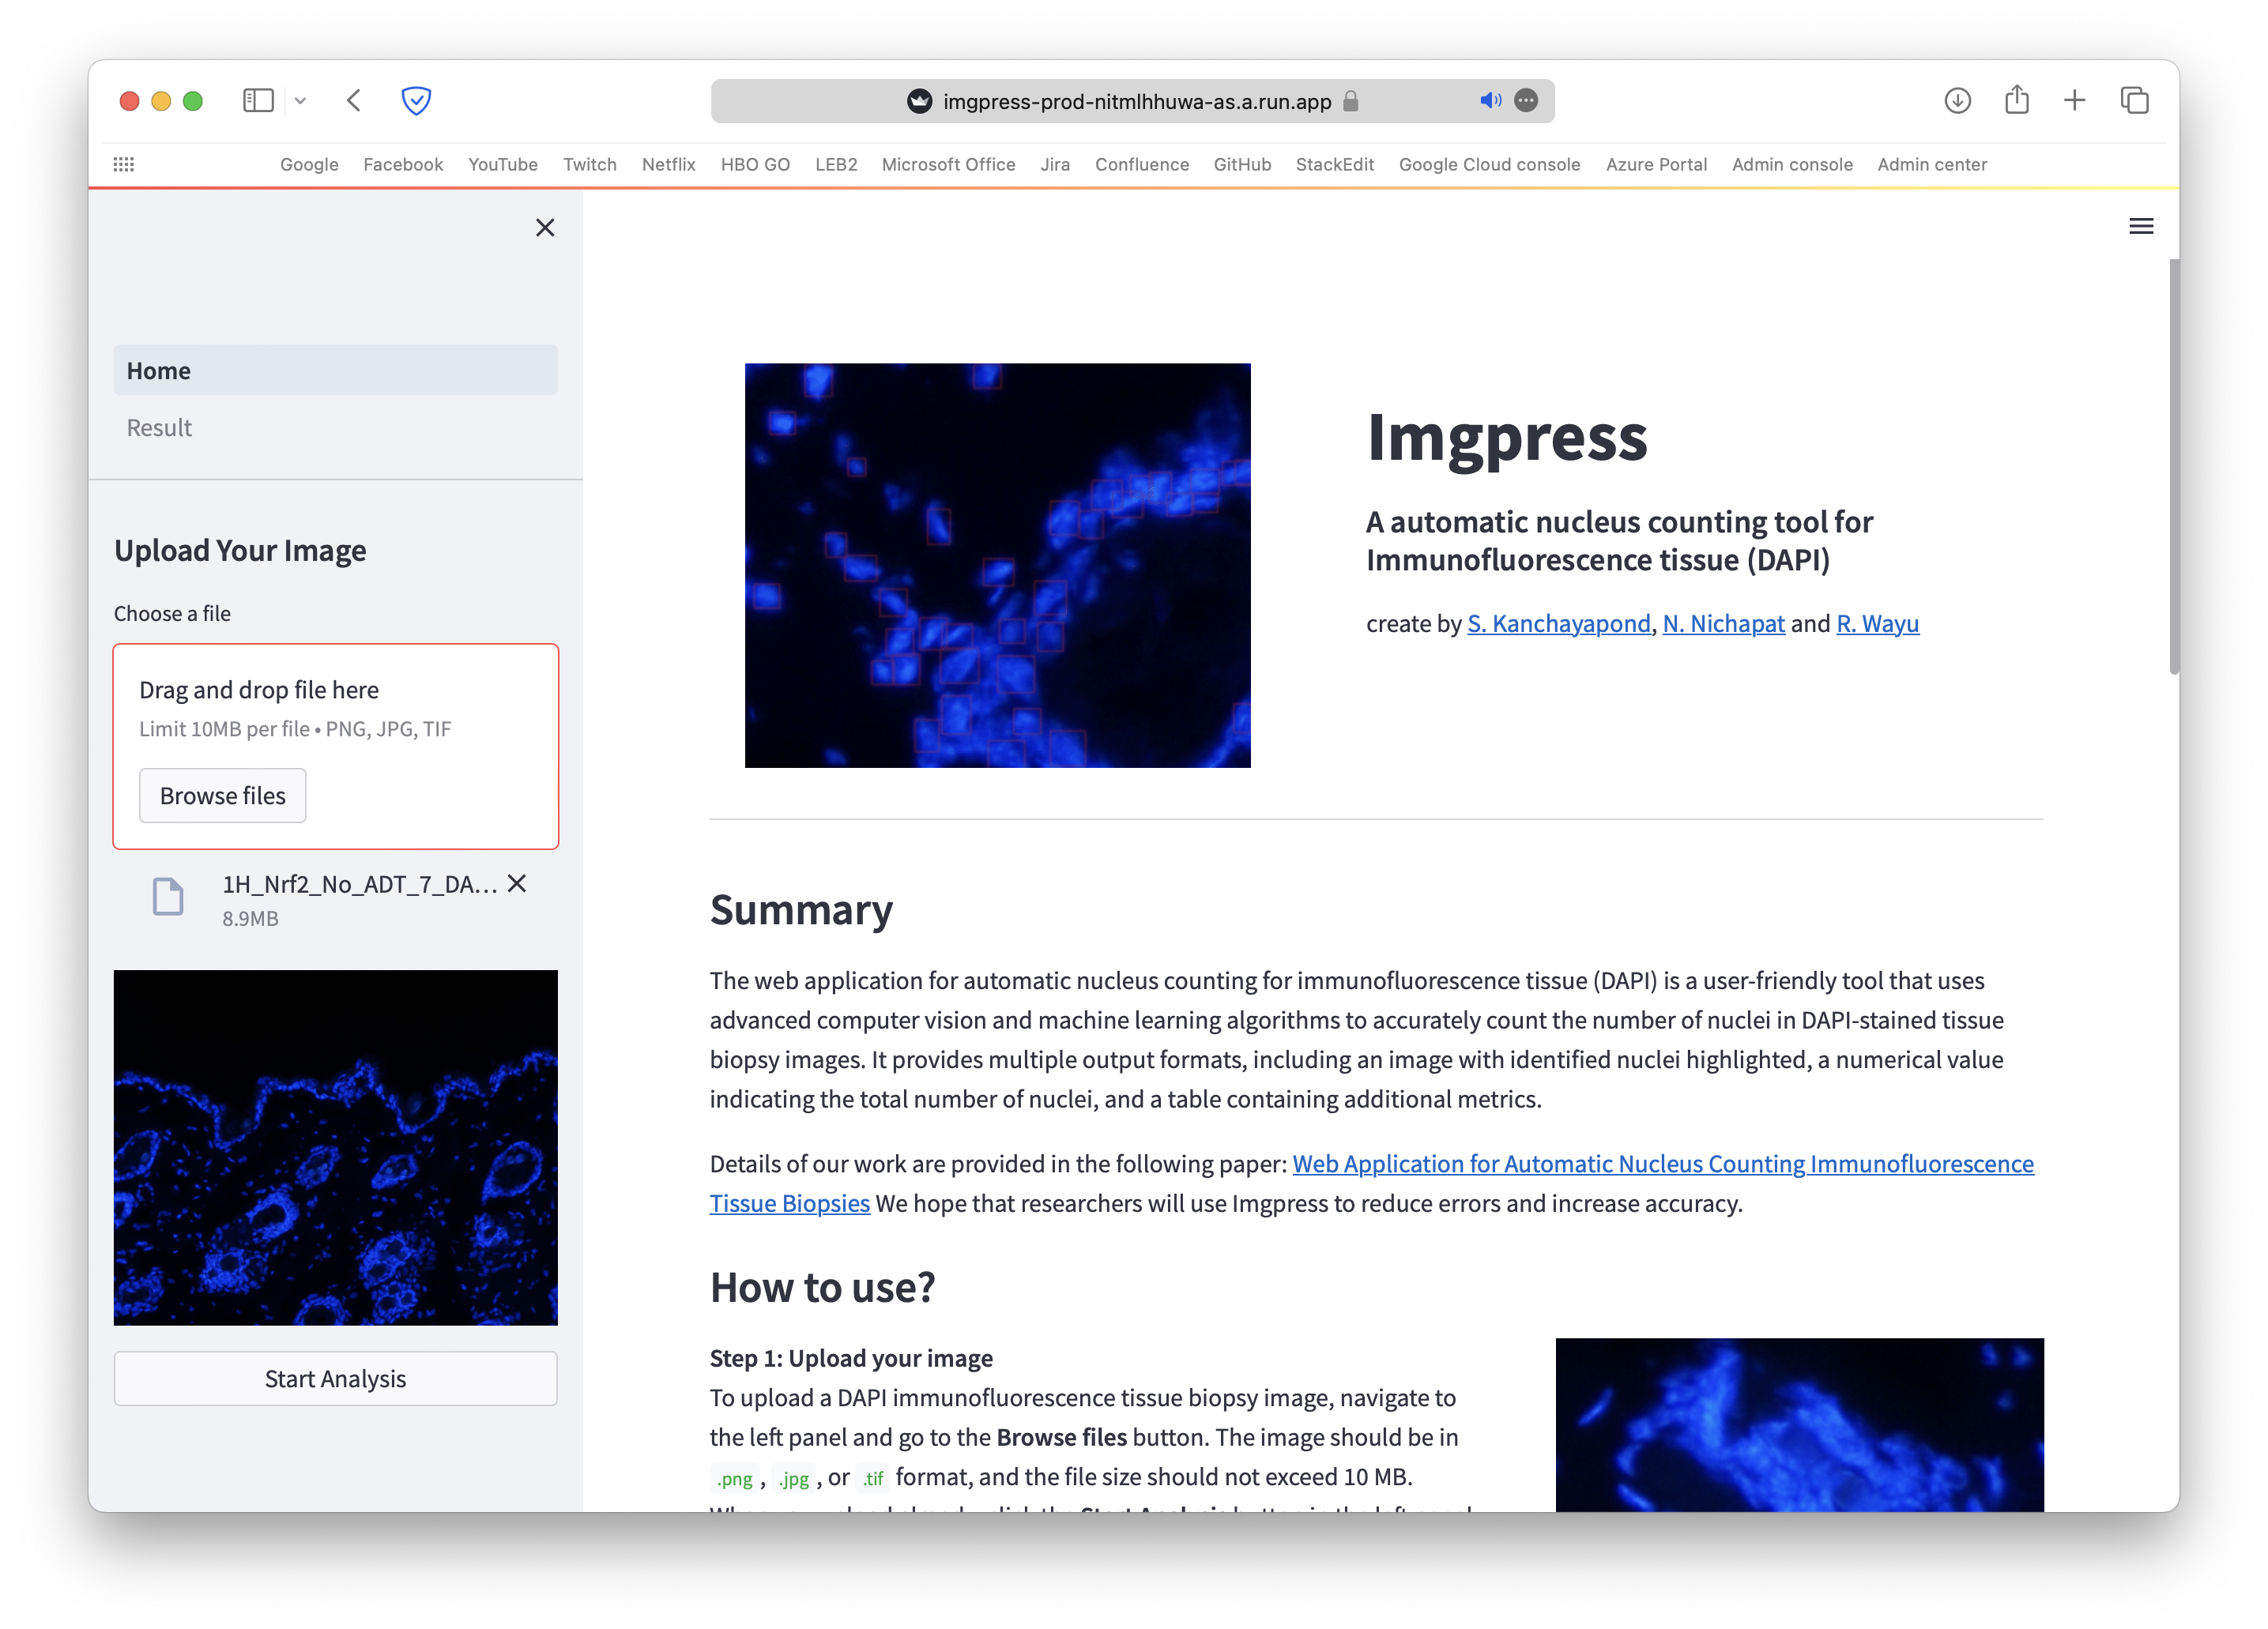
\includegraphics[width=\textwidth]{images/upload_success.png}
        % \captionsetup{justification=centering}
        \caption{รูปที่อัปโหลดจะแสดงที่บริเวณทางด้านล่าง}\label{fig:web_upload2}
    \end{subfigure}
    \caption{ส่วนอัปโหลดของเว็บแอปพลิเคชัน}
    \label{fig:uploadweb}
\end{figure}

\textbf{ส่วนผลลัพธ์}
หลังจากอัปโหลดรูป จะแสดงแถบความคืบหน้าของการทำงานของเว็บ ดังแสดงดังรูปที่~\ref{fig:web_result1} เมื่อประมวลผลเสร็จสิ้นจะนำผู้ใช้งานเข้าสู่หน้าผลลัพธ์ จะมีการบอกจำนวนของนิวเคลียสที่นับได้ทั้งหมดจากแบบจำลองอยู่บริเวณด้านบนของรูปภาพผลลัพธ์ โดยภาพผลลัพธ์จะแสดงด้านขวา และ ตารางผลลัพธ์จะแสดงในด้านซ้าย ซึ่งจะประกอบด้วย พิกัด (x, y) และ intensity ของแต่ละนิวเคลียส ดังแสดงในรูปที่~\ref{fig:web_result2} ซึ่งผู้ใช้งานสามารถย่อขยายในกรณีที่รูปมีขนาดใหญ่ สามารถครอปเลือกเพื่อขยายขนาดรูป ดังแสดงในรูปที่~\ref{fig:web_table} ผู้ใช้งานสามารถบันทึกผลลัพธ์ทั้งหมดได้ จากปุ่ม Save table และ Save Image โดยภาพผลลัพธ์จะเป็นสกุลไฟล์ png และตารางจะเป็นสกุลไฟล์ csv แต่ถ้าหากผู้ใช้งานยังไม่ได้อัปโหลดรูปในหน้าแรกของเว็บแอปพลิเคชัน หน้าผลลัพธ์จะขึ้นแจ้งเตือนให้กลับไปอัปโหลดรูปที่หน้าแรกดังแสดงในรูปที่~\ref{fig:web_warnn}
\begin{figure}[!h]
\centering
    \begin{subfigure}[b]{0.42\textwidth}
      \centering
        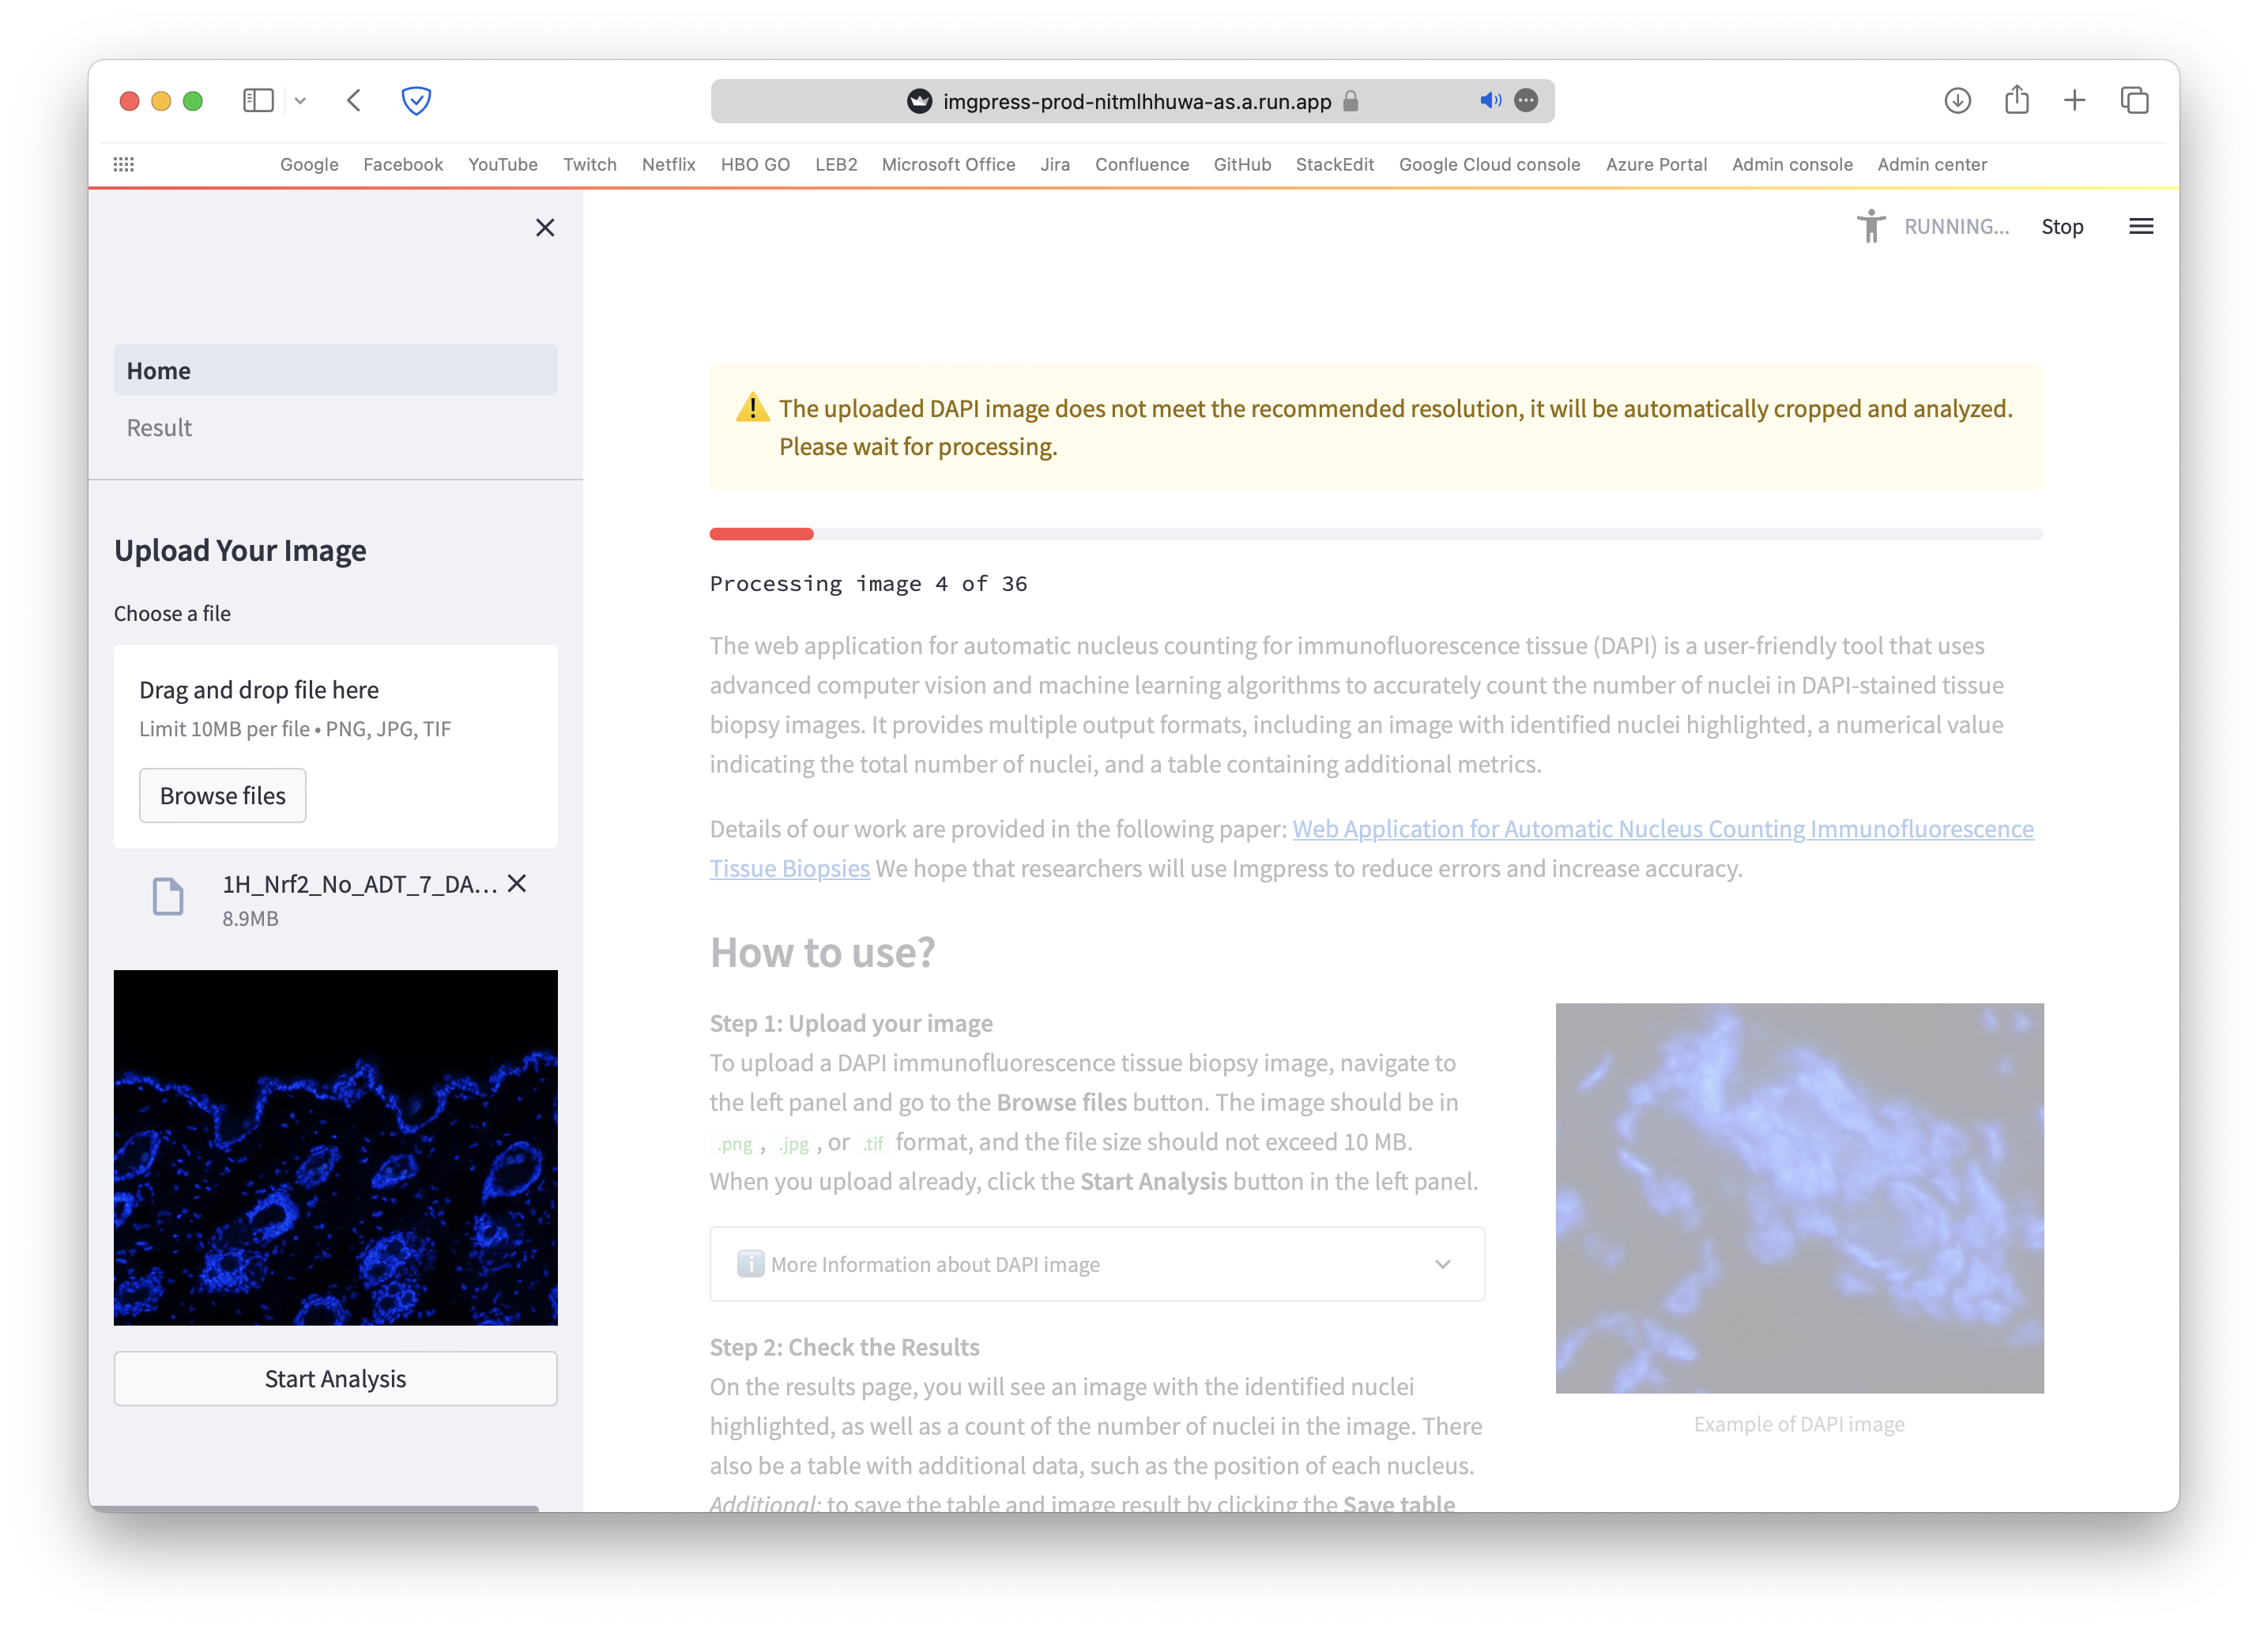
\includegraphics[width=\textwidth]{images/processing.png}
        % \captionsetup{justification=centering}
        \caption{แถบความคืบหน้าเมื่อกำลังประมวลผล}\label{fig:web_result1}
    \end{subfigure}
    \begin{subfigure}[b]{0.42\textwidth}
      \centering
        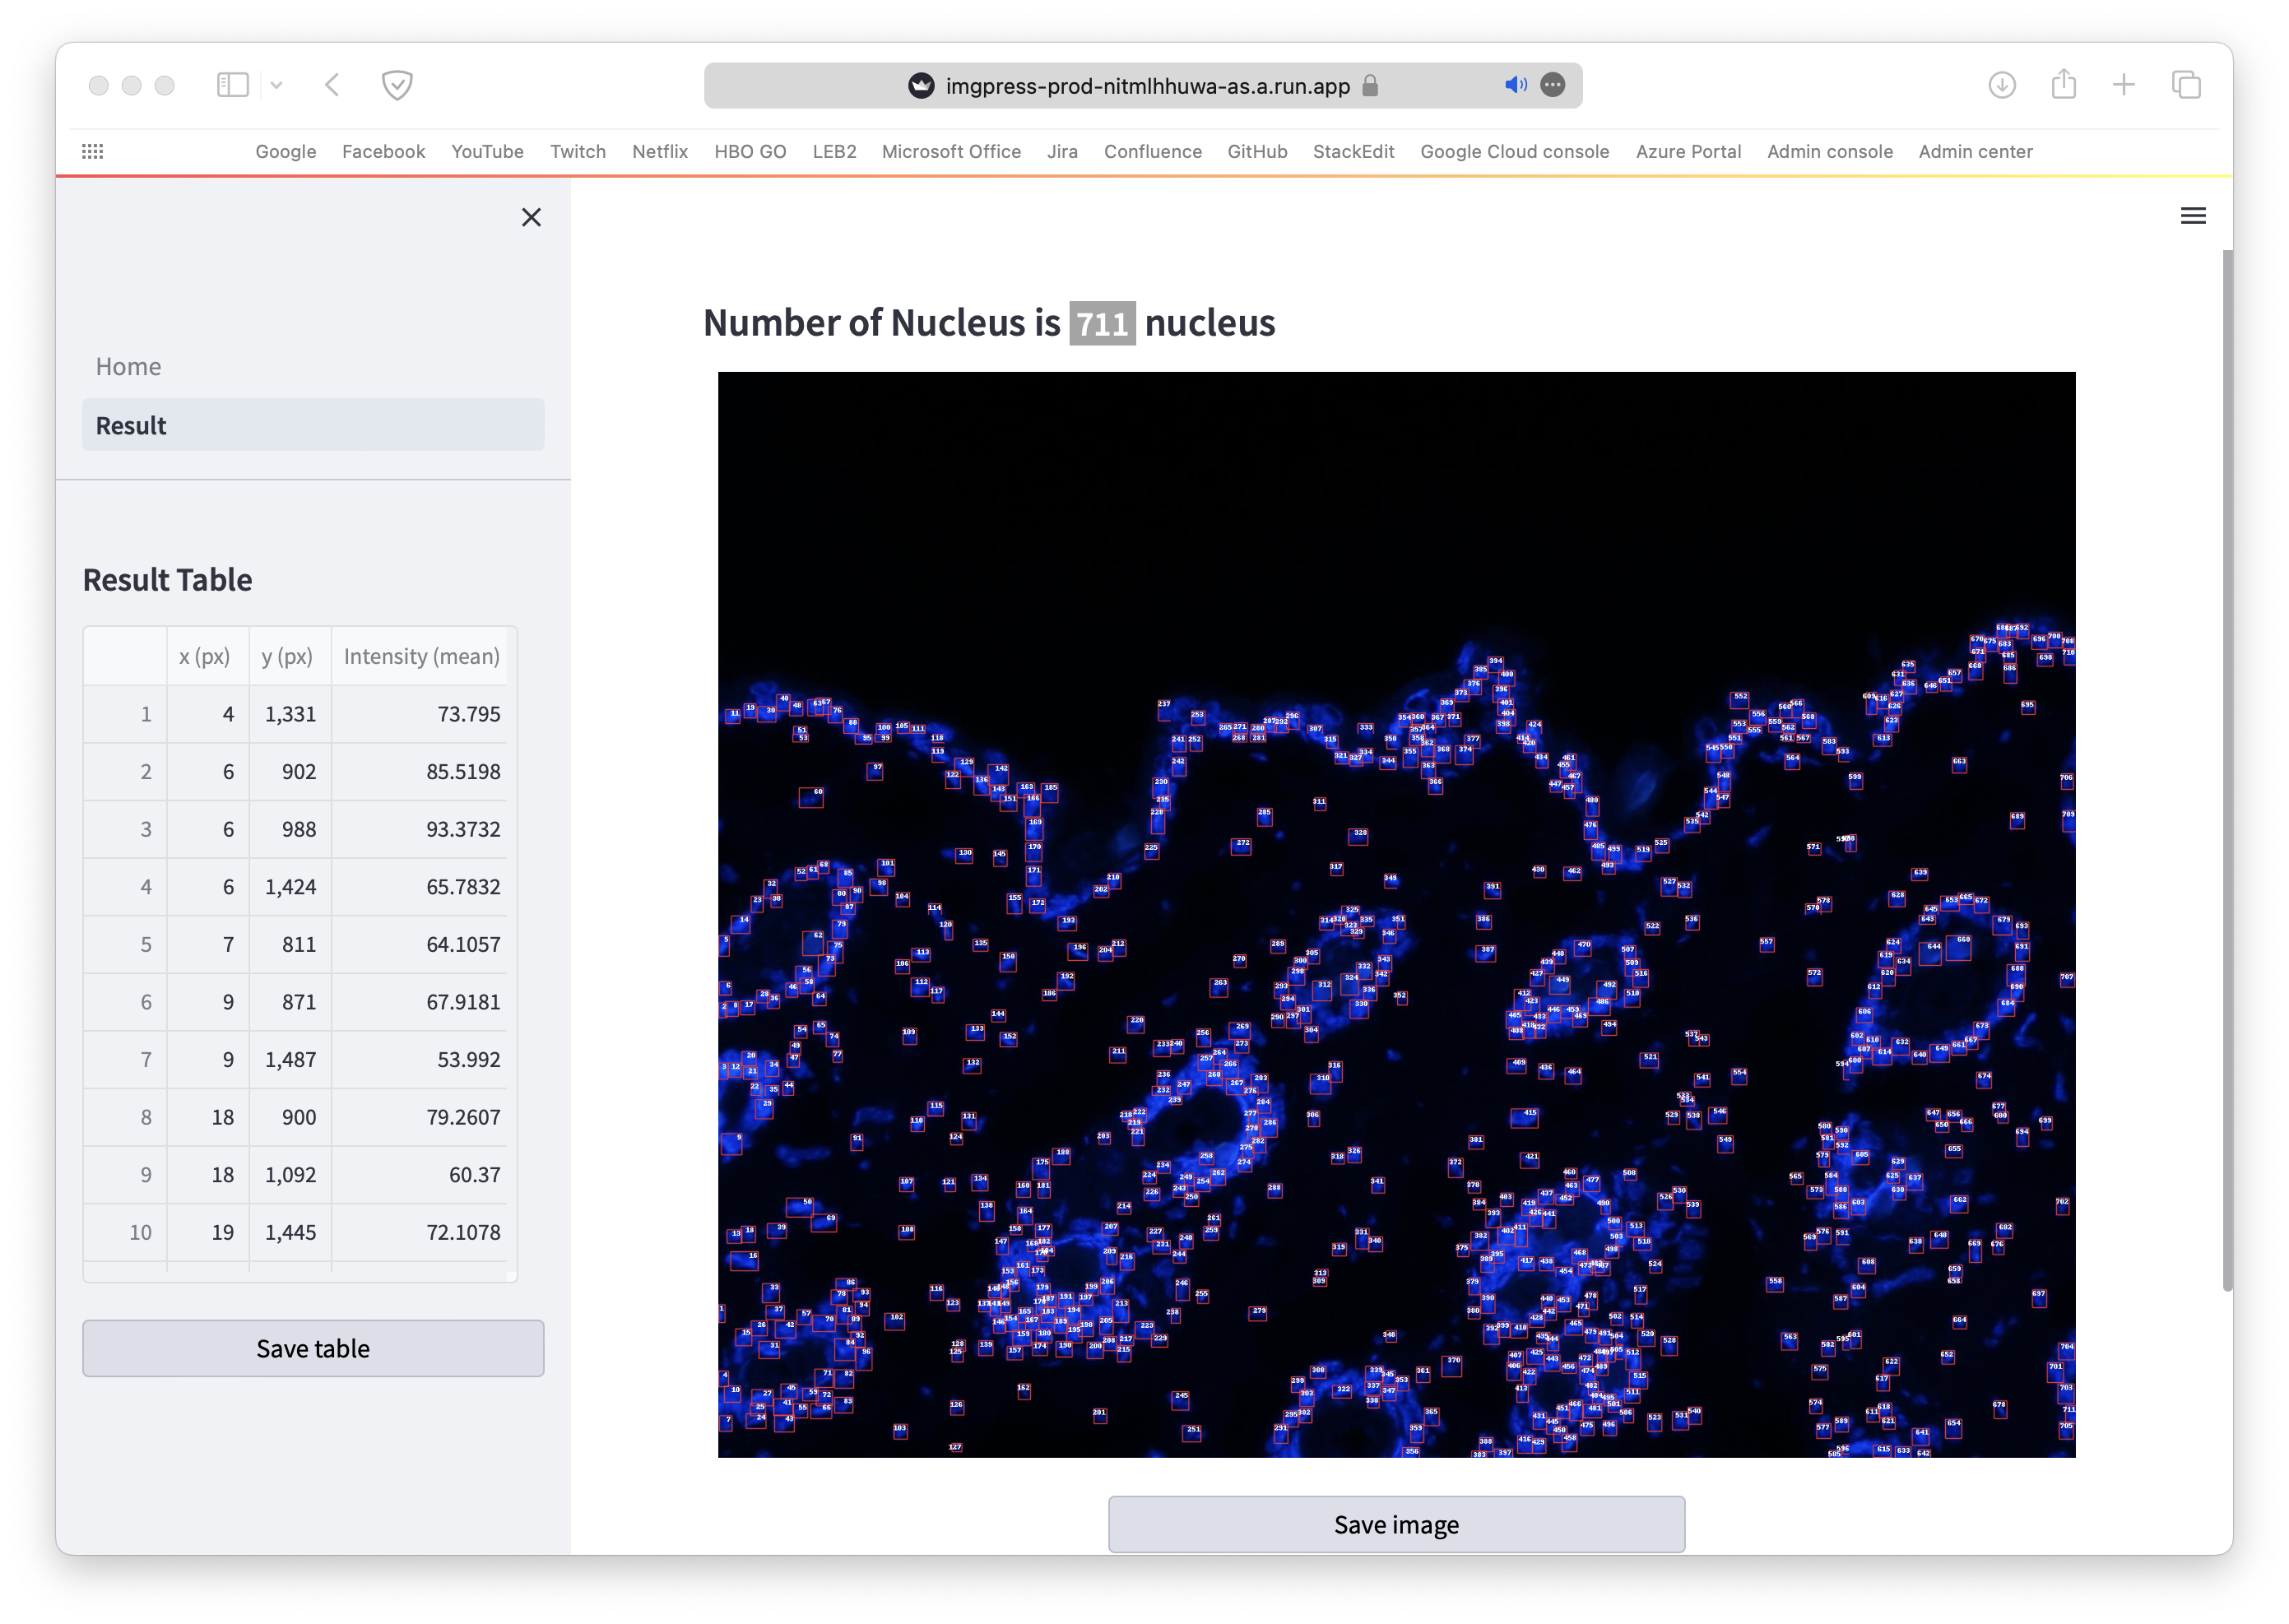
\includegraphics[width=\textwidth]{images/result.png}
        % \captionsetup{justification=centering}
        \caption{ผลลัพธ์หลังการประมวลผลเสร็จสิ้น}\label{fig:web_result2}
    \end{subfigure}
    \\[1ex]
    \begin{subfigure}[b]{0.42\textwidth}
      \centering
        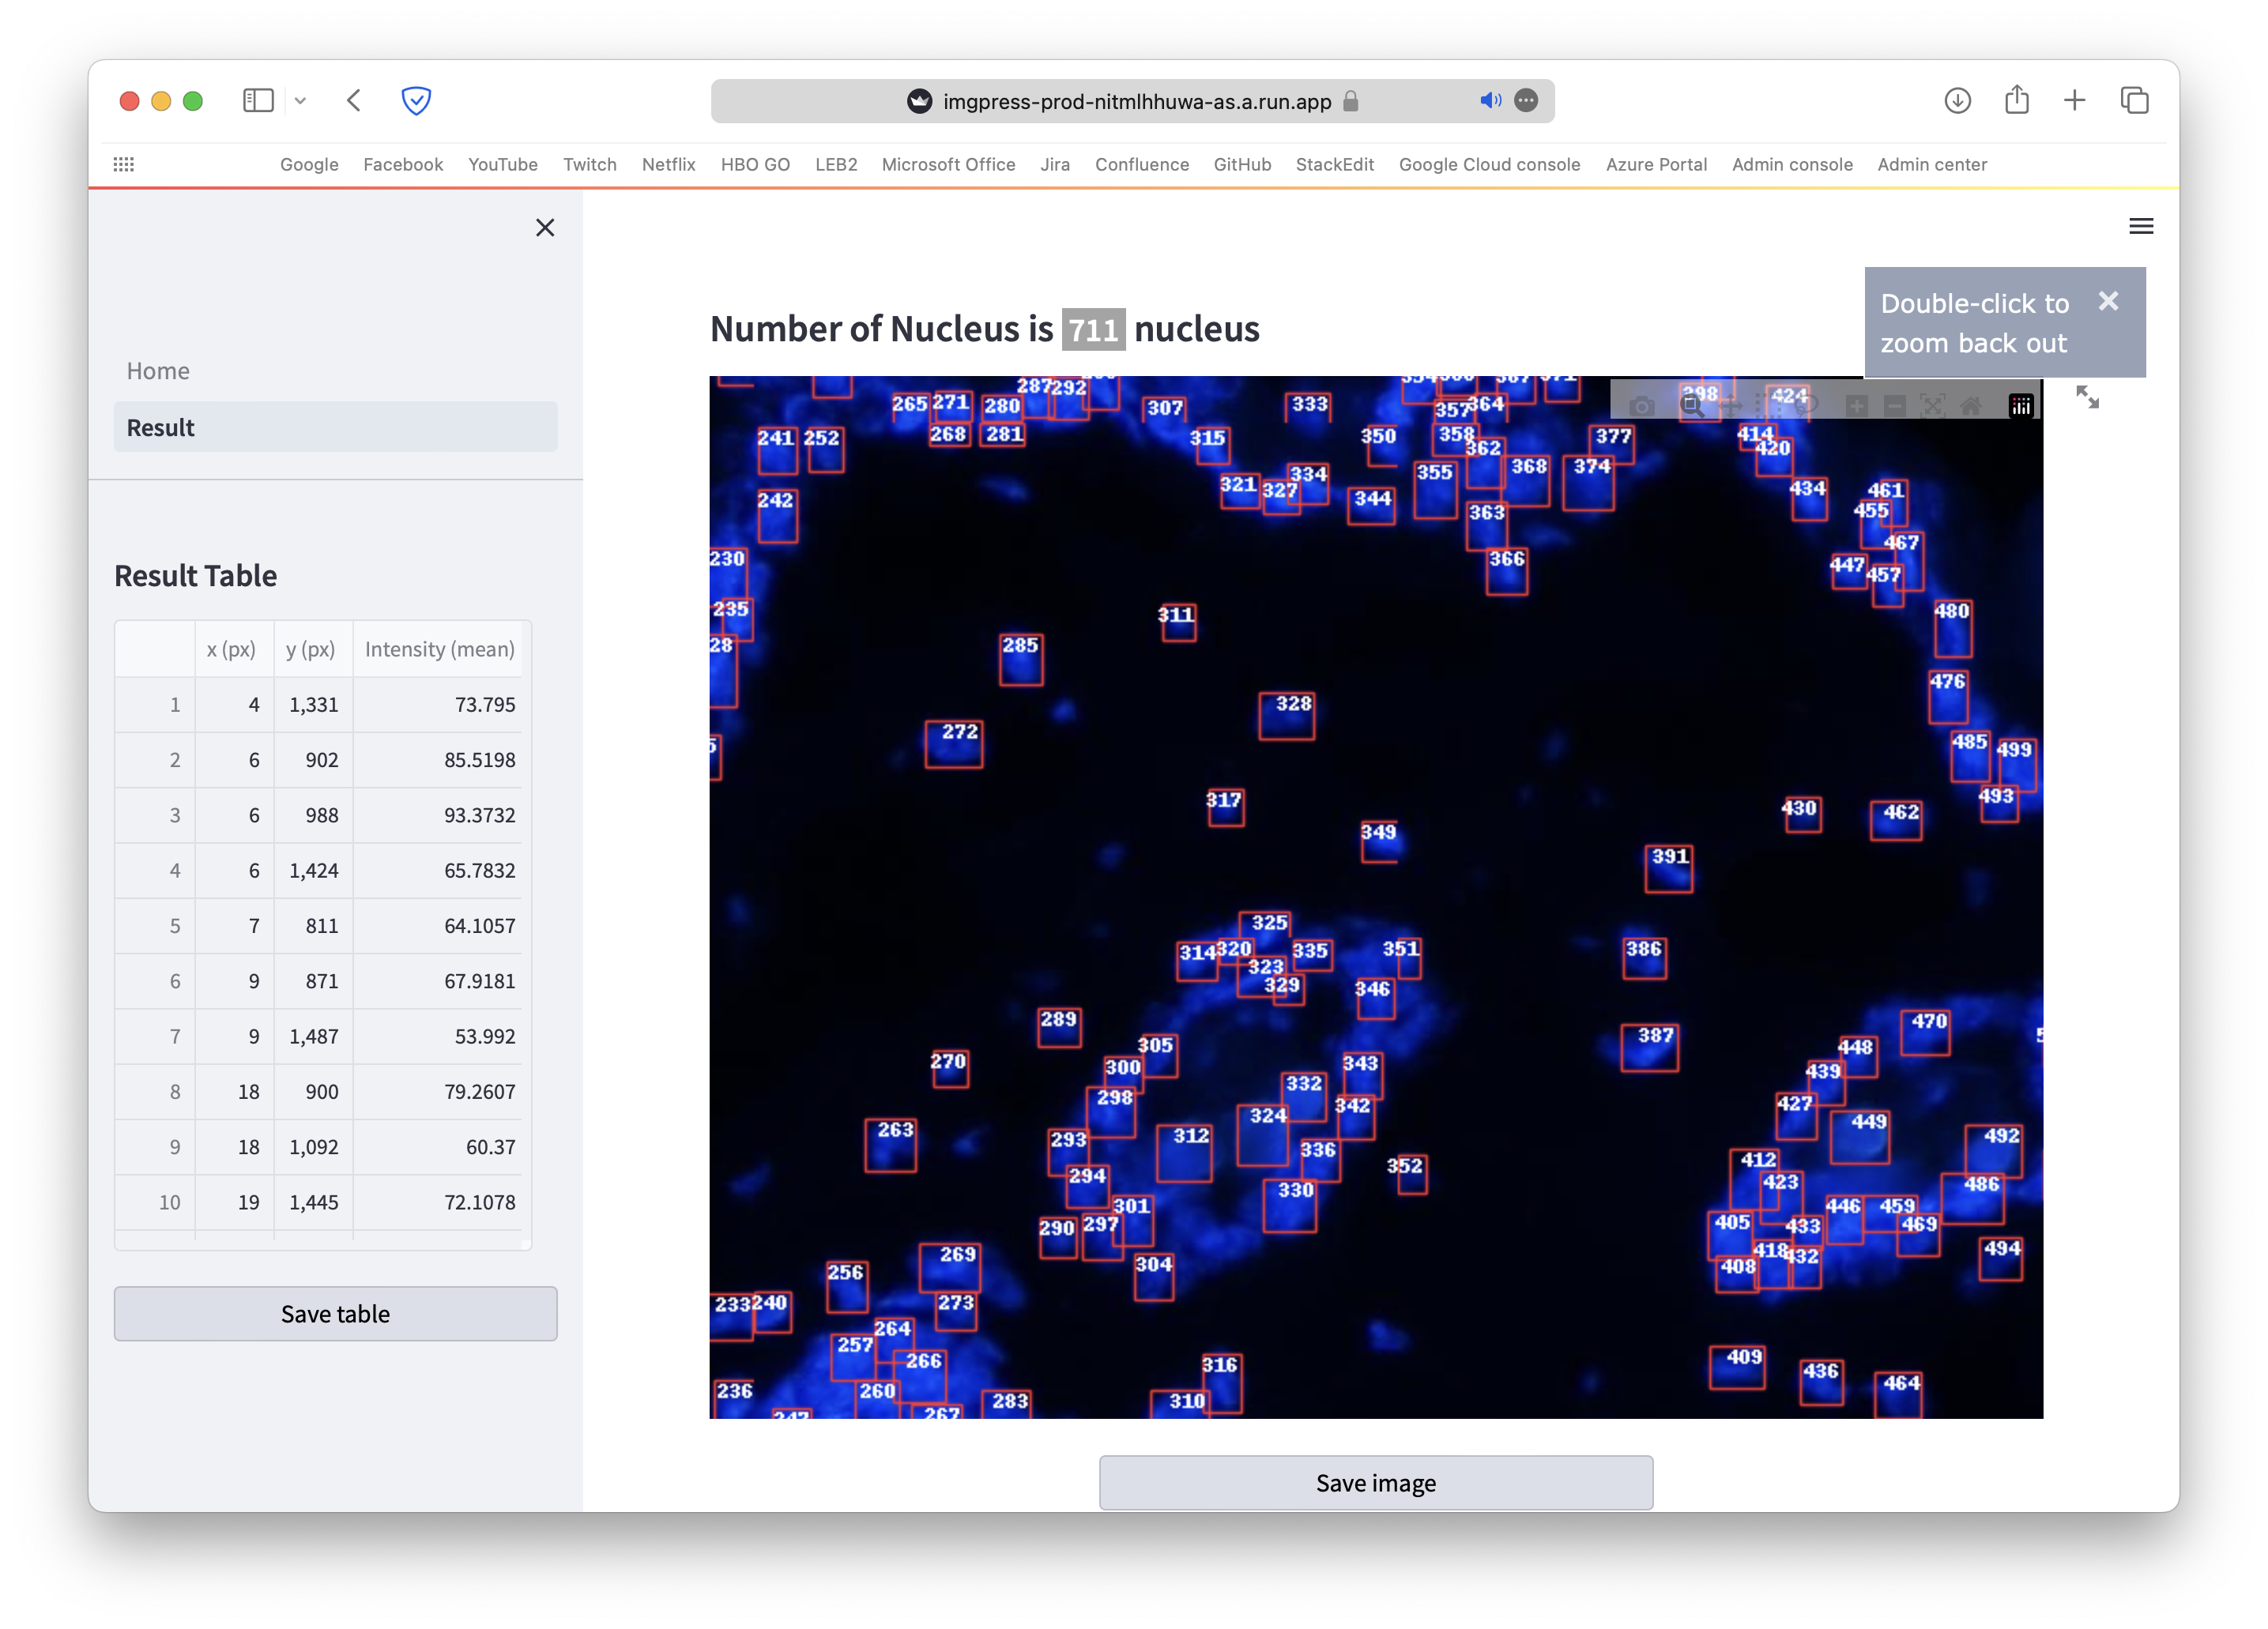
\includegraphics[width=\textwidth]{images/zoomable.png}
        % \captionsetup{justification=centering}
        \caption{ตัวอย่างการขยายภาพ}\label{fig:web_table}
    \end{subfigure}
    \begin{subfigure}[b]{0.42\textwidth}
      \centering
        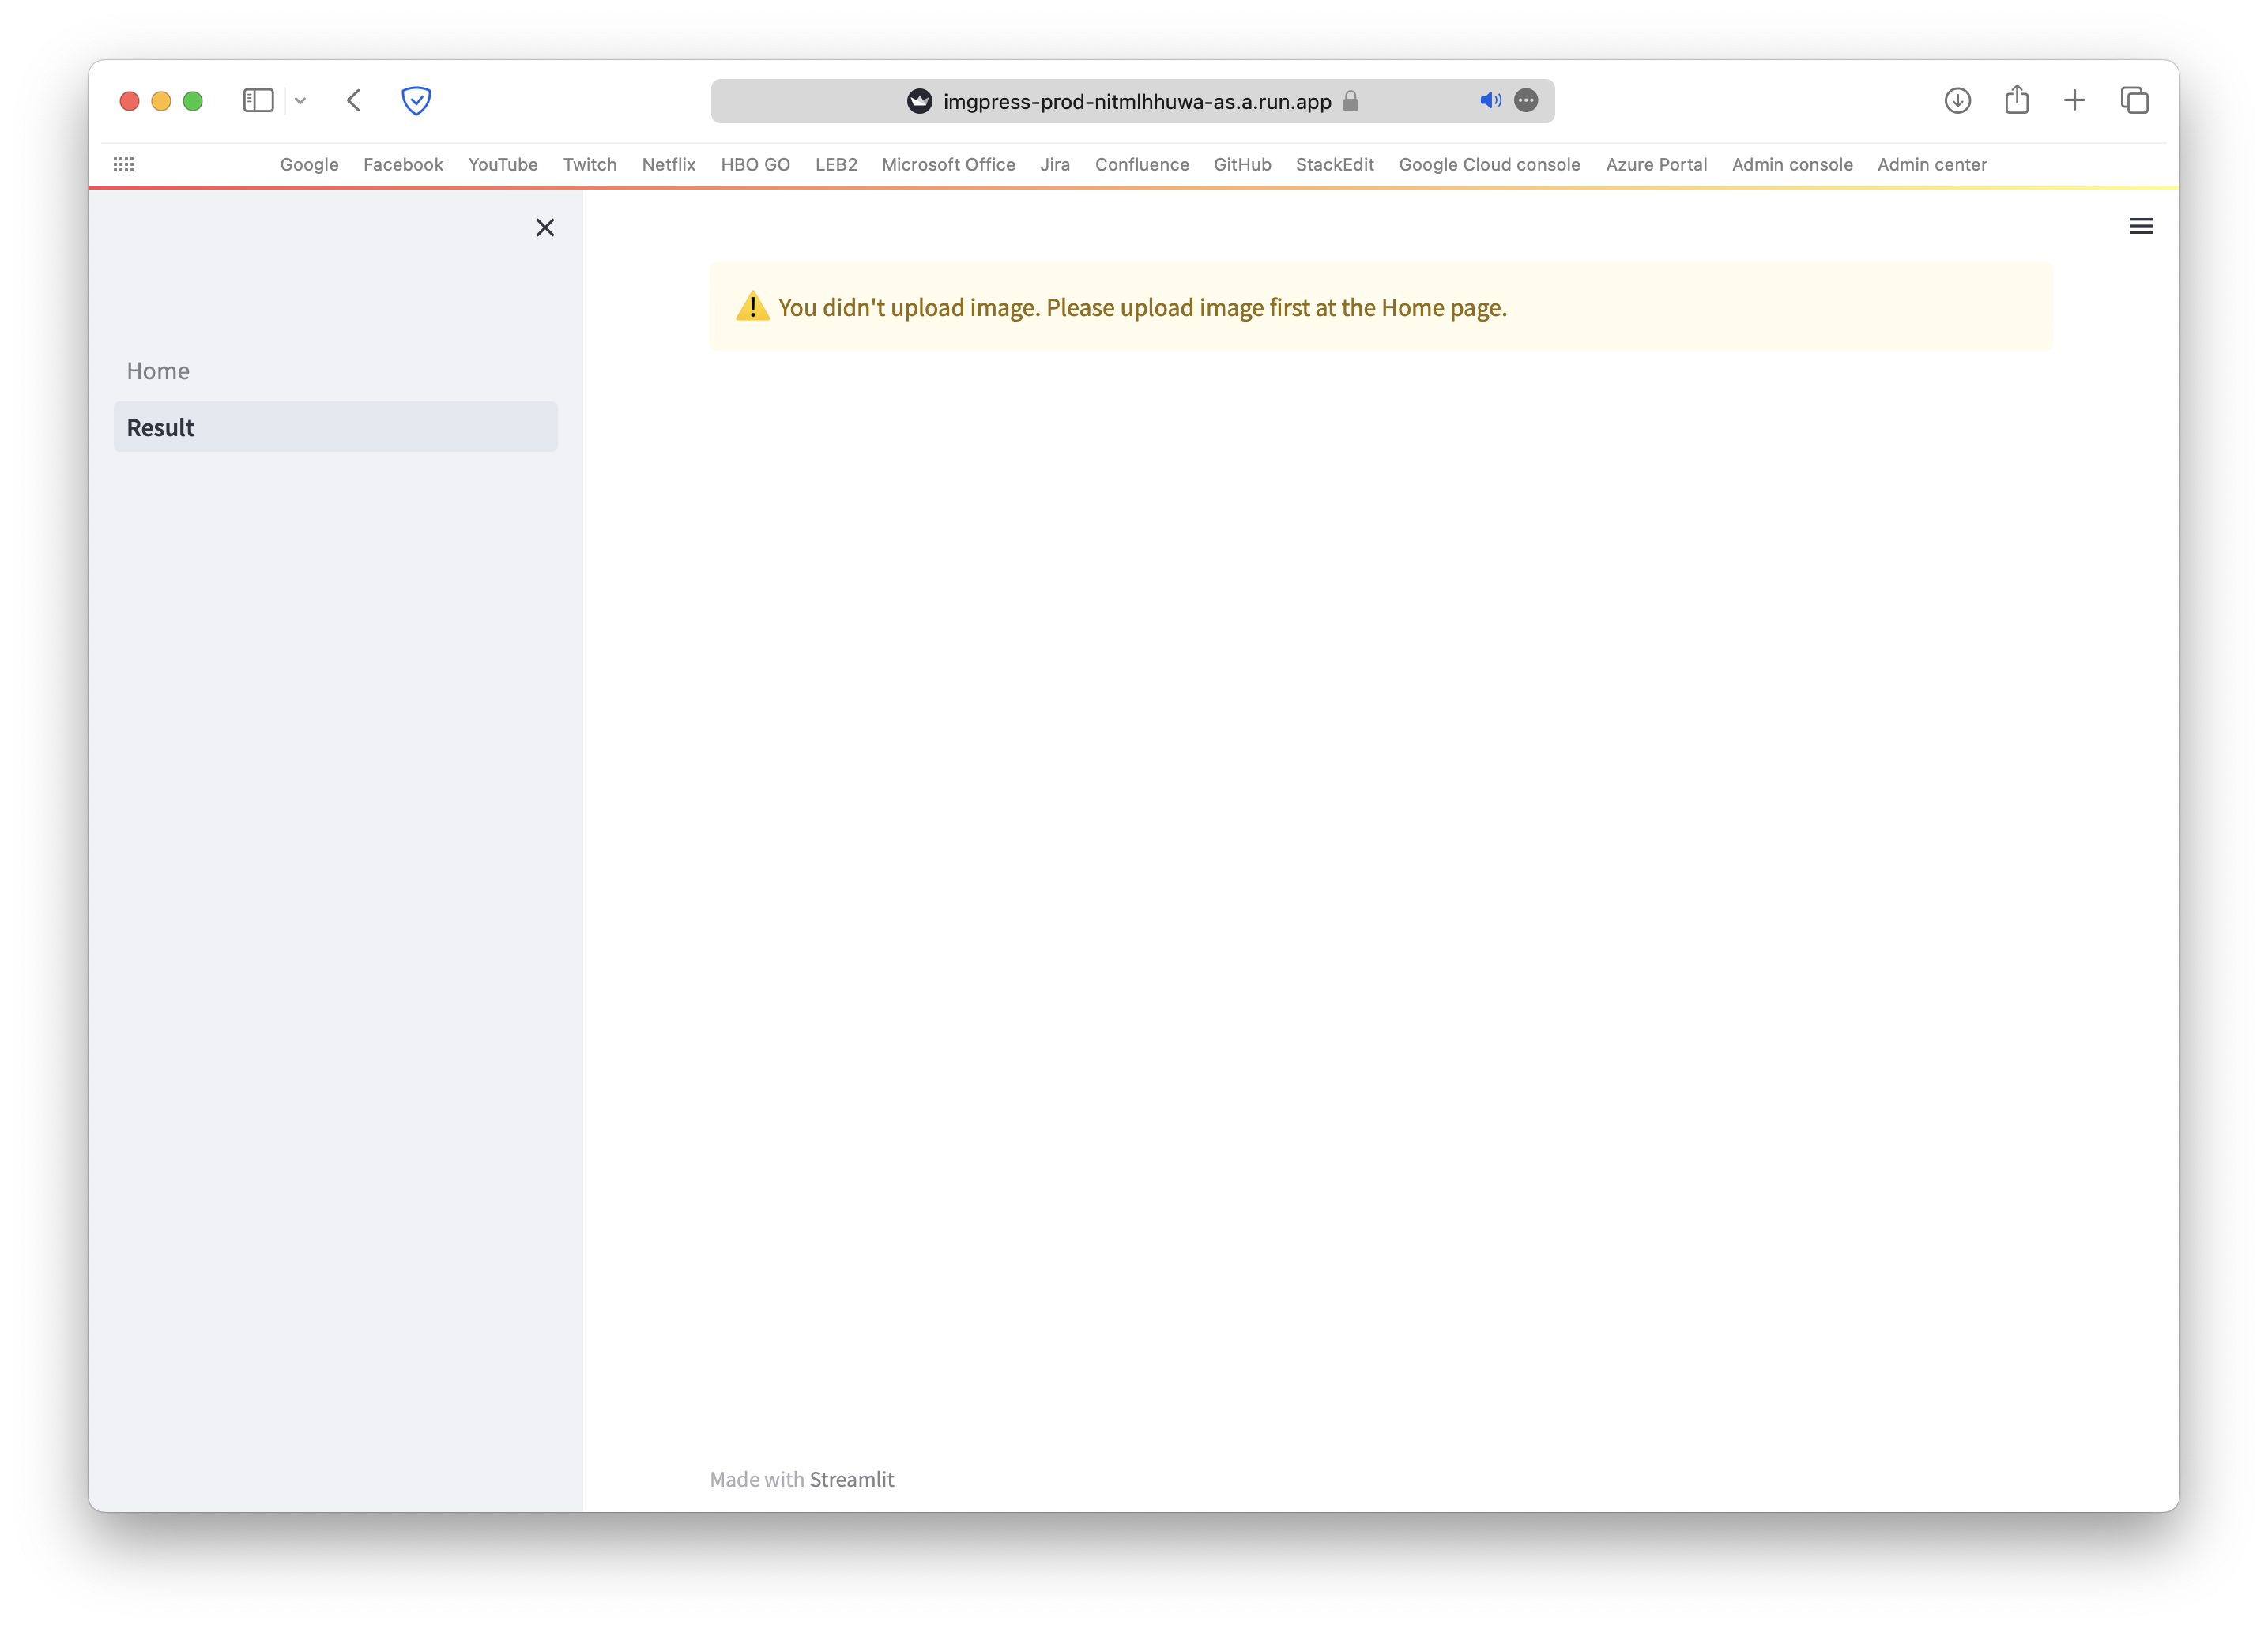
\includegraphics[width=\textwidth]{images/non_upload.png}
        % \captionsetup{justification=centering}
        \caption{ส่วนแจ้งเตือนเมื่อยังไม่ได้อัปโหลดรูป}\label{fig:web_warnn}
    \end{subfigure}
    \caption{ส่วนผลลัพธ์}
    \label{fig:resuktweb}
\end{figure}
\pagebreak
\subsection{UML Design}
หลังจากกําหนดฟังก์ชัน และรายละเอียดการทํางานของระบบนับนิวเคลียสแล้ว สามารถเขียนแผนภาพไดอะแกรมเพื่อให้สามารถเข้าใจการทํางานของระบบมากยิ่งขึ้น ด้วยแผนภาพ Use Case Diagram รูปที่~\ref{fig:uml} แสดง Use Case การทํางานของระบบทั้งหมด ซึ่งผู้ใช้งาน (User) คือ นักพยาธิวิทยาที่ต้องการจำนวนนิวเคลียส จะสามารถอัปโหลดรูปภาพ Immunofluorescence Tissue ปรับรูปแบบรูปผลลัพธ์บนหน้าว็บแอปพลิเคชัน และบันทึกรูปที่มีการ label ตำแหน่งนิวเคลียส และตารางสรุปพื้นที่ของแต่ละนิวเคลียส และเว็บแอปพลิเคชันนี้เป็นแบบ Web Automation ทำให้ไม่ต้องมีในส่วนของ Admin ในการกำกับดูแลเนื้อหาในเว็บแอปพลิเคชันนี้  
\begin{figure}[!h]\centering
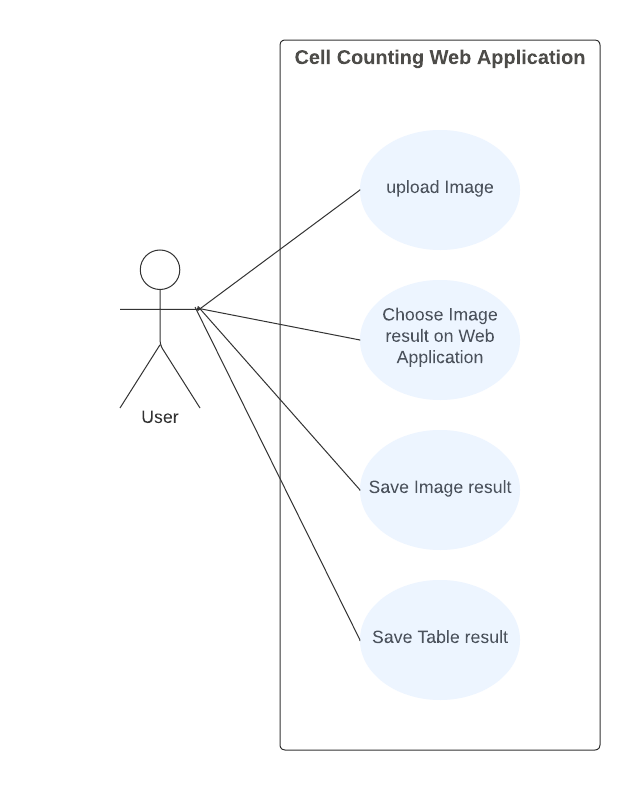
\includegraphics[width=4.5cm]{images/uml.png}
\captionsetup{justification=centering}
\caption{UML Design}\label{fig:uml}
\end{figure}
\pagebreak
\subsection{Activity Diagrams}
ต่อมาเป็นส่วนของ Activity Diagrams ซึ่งจะแสดงความสัมพันธ์ระหว่างผู้ใช้งานกับ Front-end และ Back-end ซึ่งจะมีฟังก์ชันและกระบวนการตามรูป รูปที่~\ref{fig:actty} โดยจะเริ่มจากการรับภาพจากผู้ใช้งาน แล้วจะส่งไปยัง Back-end เพื่อทำการประมวลผลภาพแล้วส่งข้อมูลออกมาเป็นจำนวนนิวเคลียส รูปที่มีการ label ตำแหน่งนิวเคลียส และตารางสรุปพื้นที่ของแต่ละนิวเคลียส ซึ่งผลลัพธ์รูปที่มีการ label ตำแหน่งนิวเคลียส ผู้ใช้งานสามารถเลือกการแสดงออกบนหน้าว็บแอปพลิเคชัน แบบแสดงรูปผลลัพธ์ขนาดใหญ่เท่าหน้าว็บแอปพลิเคชัน และแบบที่ผู้ใช้งานสามารถเลือกซูมดูภายในรูปผลลัพธ์ ต่อจากนั้นผู้ใช้งานสามารถบันทึกรูปภาพ แล้ว Back-end จะทำการส่งรูปภาพกลับมาสู่ผู้ใช้งาน อีกทั้งผู้ใช้งานยังสามารถบันทึกตาราง โดยสามารถเลือกนามสกุลไฟล์ได้ 2 แบบ คือ csv และ xlsx แล้ว Back-end จะทำการส่งตารางกลับมาสู่ผู้ใช้งาน
\begin{figure}[!h]\centering
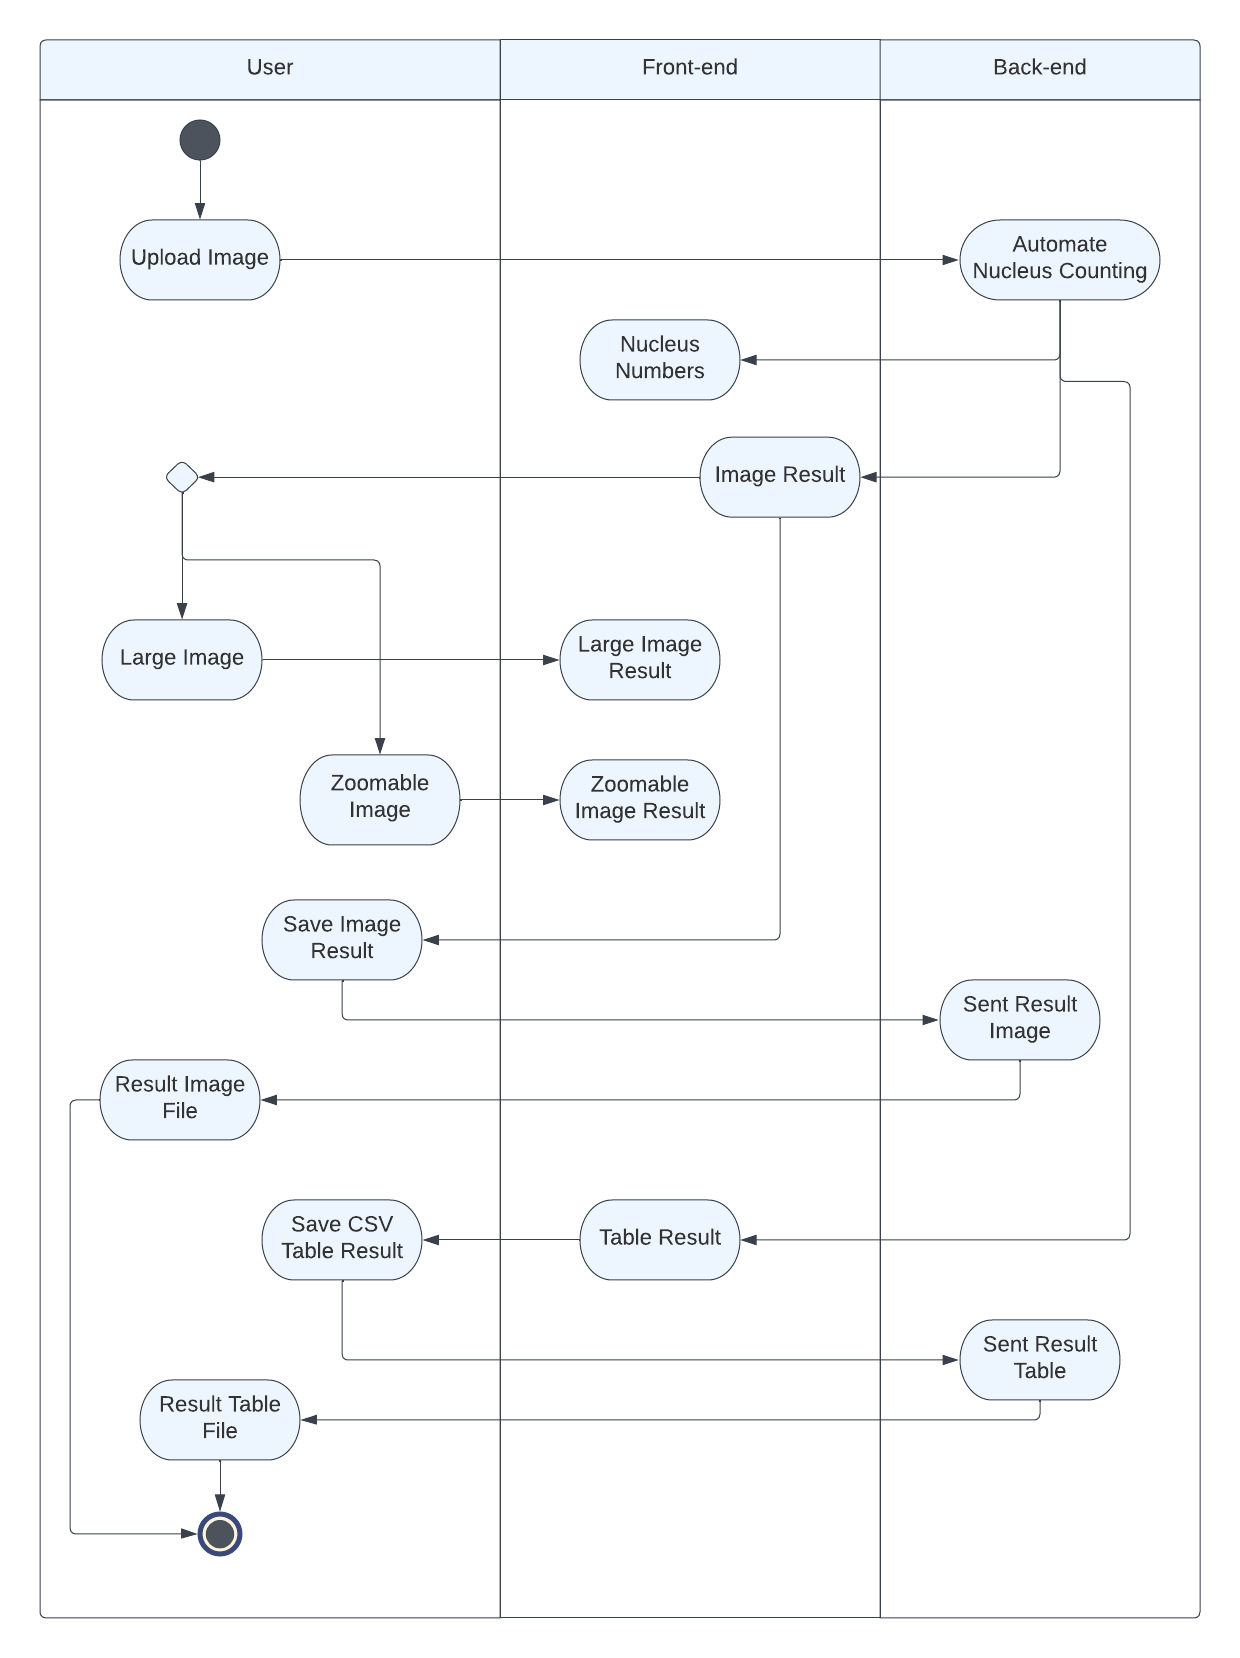
\includegraphics[width=13cm]{images/activity.png}
\captionsetup{justification=centering}
\caption{Activity Diagrams}\label{fig:actty}
\end{figure}
\subsection{แบบประเมินความพึงพอใจในการใช้เว็บแอปพลิเคชัน}
การประเมินความพึงพอใจในการใช้เว็บแอปพลิเคชันจากการใช้แบบสอบถามดังแสดงในรูปที่~\ref{fig:quationirepeople} และ ~\ref{fig:quationirepatho}จากการสัมภาษณ์ผู้ใช้งาน ได้แก่ บุคคลทั่วไป จำนวน 24 คน และนักพยาธิวิทยา จำนวน 2 คน โดยการประเมินผลความพึงพอใจต่อการใช้งานเว็บแอปพลิเคชันนั้น จะถูกแบ่งออกเป็น 3 ด้านในการประเมิน ได้แก่ ด้านการออกแบบและการจัดการรูปแบบ ด้านการใช้งาน และ ด้านการแสดงผลลัพธ์การนับจำนวนนิวเคลียส ซึ่งในแต่ละหัวข้อจะมีคำตอบได้ 5 รูปแบบ ประกอบด้วย น้อยที่สุด เท่ากับ 1 คะแนน, น้อย เท่ากับ 2 คะแนน, ปานกลาง เท่ากับ 3 คะแนน, มาก เท่ากับ 4 คะแนน และ มากที่สุด เท่ากับ 5 คะแนน โดยสรุปผลคะแนนจะนำทุกคำตอบของแบบสอบถามมาคำนวนค่าเฉลี่ย โดยหัวข้อคำถามจะผู้แบ่งออกเป็น 2 ส่วน สำหรับบุคคลทั่วไป และสำหรับนักพยาธิวิทยา มีดังนี้
\subsubsection{ชุดคำถามสำหรับบุคคลทั่วไป}
\begin{enumerate}
% \setlength{\itemindent}{.3in}
    \item ด้านการออกแบบและการจัดการรูปแบบ
    \begin{itemize}
    % \setlength{\itemindent}{.4in}

        \item    ความเหมาะสมในการเลือกใช้รูปแบบ ขนาด สีตัวอักษรบนเว็บแอปพลิเคชัน
        \item    ความเหมาะสมในการเลือกใช้ข้อความเพื่ออธิบายการใช้เว็บแอปพลิเคชัน
        \item    ความเหมาะสมในการใช้สัญลักษณ์หรือรูปภาพในการสื่อความหมาย
        \item    ความสวยงามและความทันสมัยของเว็บแอปพลิเคชัน
        \item    ความน่าสนใจของหน้าเว็บแอปพลิเคชัน
        \item    ความเหมาะสมของสีพื้นหลังที่ง่ายต่อการใช้เว็บแอปพลิเคชัน 
    \end{itemize}
    \item ด้านการแสดงผลลัพธ์การนับจำนวนนิวเคลียส
    \begin{itemize}
    % \setlength{\itemindent}{.4in}
        \item    รูปภาพผลลัพธ์และตารางมีความชัดเจนและเข้าใจง่าย
    \end{itemize}
    \item ด้านการใช้งานได้ตามฟังก์ชันการทำงาน
    \begin{itemize}
    % \setlength{\itemindent}{.4in}
        \item    การใช้คำสั่งในส่วนการอัปโหลดรูปภาพ ที่ง่ายต่อการใช้งาน
        \item    การใช้คำสั่งในการบันทึกผลลัพธ์ที่ได้ลงอุปกรณ์ของตนเอง ที่ง่ายต่อการใช้งาน
        \item    การใช้คำสั่งการย่อ/ขยายรูปผลลัพธ์ ที่ง่ายต่อการใช้งาน
        \item    ความเร็วในการประมวลผลของเว็บแอปพลิเคชัน
        \item    ประโยชน์ในการใช้งานเว็บแอปพลิเคชัน
        \item    ภาพรวมของเว็บแอปพลิเคชันตรงต่อความต้องการของผู้ใช้
    \end{itemize}
\end{enumerate}


\subsubsection{ชุดคำถามสำหรับนักพยาธิวิทยา}
\begin{enumerate}
% \setlength{\itemindent}{.3in}
    \item ด้านการออกแบบและการจัดการรูปแบบ
    \begin{itemize}
    % \setlength{\itemindent}{.4in}

        \item    ความเหมาะสมในการเลือกใช้รูปแบบ ขนาด สีตัวอักษรบนเว็บแอปพลิเคชัน
        \item    ความเหมาะสมในการเลือกใช้ข้อความเพื่ออธิบายการใช้เว็บแอปพลิเคชัน
        \item    ความเหมาะสมในการใช้สัญลักษณ์หรือรูปภาพในการสื่อความหมาย
        \item    ความสวยงามและความทันสมัยของเว็บแอปพลิเคชัน
        \item    ความน่าสนใจของหน้าเว็บแอปพลิเคชัน
        \item    ความเหมาะสมของสีพื้นหลังที่ง่ายต่อการใช้เว็บแอปพลิเคชัน 
    \end{itemize}
    \item ด้านการแสดงผลลัพธ์การนับจำนวนนิวเคลียส
    \begin{itemize}
    % \setlength{\itemindent}{.4in}
        \item    ผลลัพธ์ที่ได้จากการทำนายมีความชัดเจนและตรงกับความต้องการของผู้ใช้
        \item    ผลลัพธ์มีความถูกต้อง
        \item    ขนาดของรูปผลลัพธ์มีขนาดที่ความเหมาะสมต่อการมองเห็น
    \end{itemize}
    \item ด้านการใช้งานได้ตามฟังก์ชันการทำงาน
    \begin{itemize}
    % \setlength{\itemindent}{.4in}
        \item    การใช้คำสั่งในส่วนการอัปโหลดรูปภาพ ที่ง่ายต่อการใช้งาน
        \item    การใช้คำสั่งในการบันทึกผลลัพธ์ที่ได้ลงอุปกรณ์ของตนเอง ที่ง่ายต่อการใช้งาน
        \item    การใช้คำสั่งการย่อ/ขยายรูปผลลัพธ์ ที่ง่ายต่อการใช้งาน
        \item    ความเร็วในการประมวลผลของเว็บแอปพลิเคชัน
        \item    ประโยชน์ในการใช้งานเว็บแอปพลิเคชัน
        \item    ภาพรวมของเว็บแอปพลิเคชันตรงต่อความต้องการของผู้ใช้
    \end{itemize}
\end{enumerate}
\begin{figure}[!h]\centering
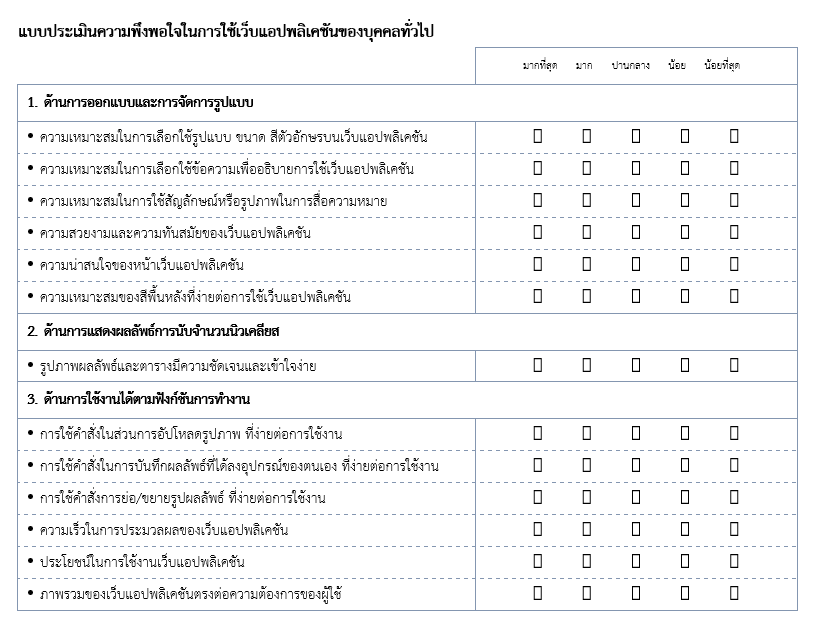
\includegraphics[width=14cm]{images/questionnairepeople.png}
\captionsetup{justification=centering}
\caption{แบบประเมินความพึงพอใจในการใช้เว็บแอปพลิเคชันบุคคลทั่วไป}\label{fig:quationirepeople}
\end{figure}

\begin{figure}[!h]\centering
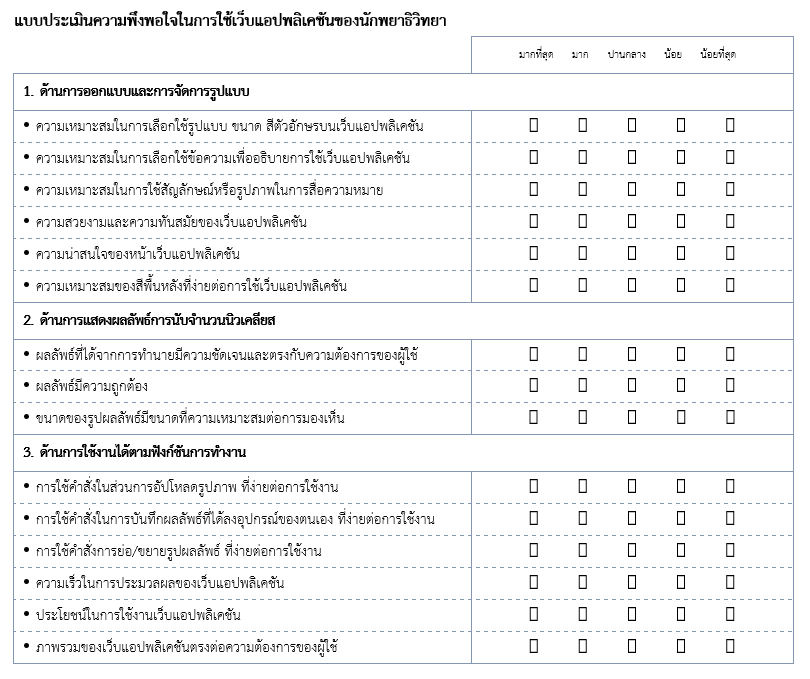
\includegraphics[width=14cm]{images/questionnairepatho.png}
\captionsetup{justification=centering}
\caption{แบบประเมินความพึงพอใจในการใช้เว็บแอปพลิเคชันของนักพยาธิวิทยา}\label{fig:quationirepatho}
\vspace{128in}
\end{figure}






%%%%%%%%%%%%%%%%%%%%%%%%%%%%%%%%%%%%%%%%%%%%%%%%%%%%%%%%%%%%%%
%%%%%%%%%%%%%%%%%%%% Experiments %%%%%%%%%%%%%%%%%%%%%%%%%%%%%
%%%%%%%%%%%%%%%%%%%%%%%%%%%%%%%%%%%%%%%%%%%%%%%%%%%%%%%%%%%%%%%
\chapter{ผลการดำเนินงาน}

\section{การวิเคราะห์ข้อมูลและผลการทดลอง}
\subsection{การทดลองแต่ละแบบจำลองและปรับพารามิเตอร์}
โดยการทดลองนี้ได้ทำการทดลองกับแบบจำลองการเรียนรู้เชิงลึกทั้งหมด 3 แบบจำลองได้แก่ Mask R-CNN, YOLO, U-Net และการประมวลผลภาพ (Image Processing) 
\subsubsection{Mask R-CNN}
การทดลองปรับพารามิเตอร์ของแบบจำลอง Mask R-CNN คณะผู้วิจัยได้ทำการทดลองทั้งหมด 2 พารามิเตอร์ โดยในแต่ละพารามิเตอร์จะทำการทดลองปรับค่าพารามิเตอร์เพื่อให้ได้ค่าพารามิเตอร์ที่ทำให้แบบจำลองมีผลลัพธ์ดีที่สุดซึ่งคือ Precision, Recall, F1 Score, ENr และ DSC ได้ค่าการวัดผลที่ดีที่สุด ซึ่งจากตารางที่ \ref{tbl:MaskR-CNNresult}  พบว่าการปรับพารามิเตอร์ momentum เท่ากับ 0.3 ได้ผลลัพธ์ที่ดีที่สุด ตัวอย่างผลลัพธ์จากแบบจำลอง Mask R-CNN แสดงดังรูปที่~\ref{fig:three maskrcnnresult}
\begin{figure}[!h]
     \centering
     \begin{subfigure}[b]{0.3\textwidth}
         \centering
         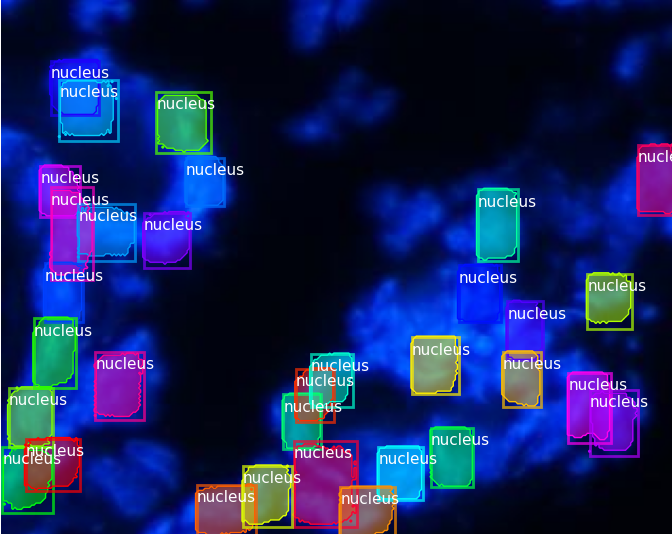
\includegraphics[width=\textwidth]{images/maskrcnn_ADT_3_3.png}
     \end{subfigure}
     \hfill
     \begin{subfigure}[b]{0.3\textwidth}
         \centering
         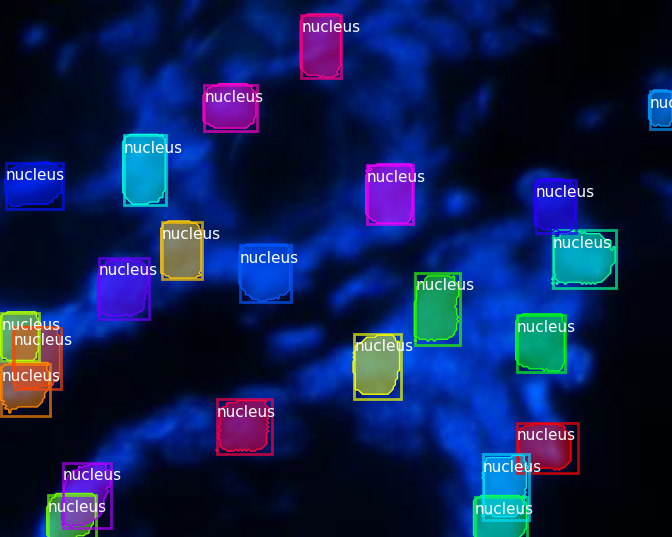
\includegraphics[width=\textwidth]{images/maskrcnn_AP123_4_1_1.png}
     \end{subfigure}
     \hfill
     \begin{subfigure}[b]{0.3\textwidth}
         \centering
         \includegraphics[width=\textwidth]{images/maskrcnn_AP39_3_3.png}
     \end{subfigure}
        \caption{ผลลัพธ์จากแบบจำลอง Mask R-CNN}
        \label{fig:three maskrcnnresult}
\end{figure}

\begin{table}[h!]
\caption{ตารางผลการทดสอบของแบบจำลอง Mask R-CNN}\label{tbl:MaskR-CNNresult}
\begin{tabular}{>{\raggedright}p{0.35\textwidth}>{\centering}p{0.1\textwidth}>{\centering}p{0.1\textwidth}>{\centering}p{0.1\textwidth}>{\centering}p{0.1\textwidth}>{\centering\arraybackslash}p{0.1\textwidth}}
\toprule
\textbf{Method}      & \textbf{Precision} & \textbf{Recall} & \textbf{F1 Score} & \textbf{ENr} & \textbf{DSC}   \\ \midrule
Base      &  0.904	& 0.465	& 0.601  & 0.502 & 0.537      \\
Non-maximum Suppression(NMS)= 0.5      &  \textbf{0.941} &	0.409 &	0.547 & 0.456 & 0.509      \\ momentum = 0.3      &  0.857 &	\textbf{0.581}	& \textbf{0.693} & \textbf{0.659} & 0.571      \\ \bottomrule 
\end{tabular}
\end{table}
\subsubsection{YOLO}
การทดลองปรับพารามิเตอร์ของแบบจำลอง YOLO คณะผู้วิจัยได้ทำการทดลองทั้งหมด 6 พารามิเตอร์และการทดลองกับทั้ง 6 ฟังก์ชันในหนึ่งการทดลอง โดยในแต่ละฟังก์ชันทำการทดลองปรับค่าพารามิเตอร์เพื่อให้ได้ค่าพารามิเตอร์ที่ทำให้แบบจำลองมีผลลัพธ์ค่าการวัดผลที่ดีที่สุดซึ่งคือ Precision, Recall, F1 Score, ENr และ DSC ได้ค่ามากที่สุด ซึ่งจากตารางที่ \ref{tbl:YOLOresult}  พบว่าการใส่ทั้ง 6 พารามิเตอร์ได้ค่าการวัดผลได้ผลลัพธ์ที่ดีที่สุด ตัวอย่างผลลัพธ์จากแบบจำลอง YOLO แสดงดังรูปที่~\ref{fig:three yoloresult}
\begin{figure}[!h]
     \centering
     \begin{subfigure}[b]{0.3\textwidth}
         \centering
         \includegraphics[width=\textwidth]{images/yoloresult.png}
     \end{subfigure}
     \hfill
     \begin{subfigure}[b]{0.3\textwidth}
         \centering
         \includegraphics[width=\textwidth]{images/yoloresult2.png}
     \end{subfigure}
     \hfill
     \begin{subfigure}[b]{0.3\textwidth}
         \centering
         \includegraphics[width=\textwidth]{images/yoloresult3.png}
     \end{subfigure}
        \caption{ผลลัพธ์จากแบบจำลอง YOLO}
        \label{fig:three yoloresult}
\end{figure}

\begin{table}[!h]
\caption{ตารางผลการทดสอบของแบบจำลอง YOLO}\label{tbl:YOLOresult}
\begin{tabular}{>{\raggedright}p{0.35\textwidth}>{\centering}p{0.1\textwidth}>{\centering}p{0.1\textwidth}>{\centering}p{0.1\textwidth}>{\centering}p{0.1\textwidth}>{\centering\arraybackslash}p{0.1\textwidth}}
\toprule
\textbf{Method}      & \textbf{Precision} & \textbf{Recall} & \textbf{F1 Score} & \textbf{ENr} & \textbf{DSC}   \\ \midrule
Base      &  0.802 & 0.862 &	0.831  & 0.907 & 0.710    \\
Dropout = 0.1      &  0.802	&	0.862	& 0.831 & \textbf{0.918} & 0.708      \\
Leaky = 0.1     &  0.831 &	0.890 &	0.859 & 0.881 & 0.687   \\
Hardswish   &  0.802 &  0.862 &	0.831 & \textbf{0.918} & 0.708 \\ 
momentum = 0.90  &  0.840 &	0.813 &	0.826 & 0.826 & 0.708\\
scale image = 0.8      &  0.859 &	0.888 &	0.873 & 0.859 & 0.708 \\
object loss = 0.5     &  0.826 &	0.805 &	0.815 & 0.719 & 0.683	\\ 
All of changed parameters      &  \textbf{0.896} &	\textbf{0.908} &	\textbf{0.902} & 0.823 & \textbf{0.713} \\ \bottomrule
\end{tabular}
\end{table}
\pagebreak
\subsubsection{U-Net}
การทดลองปรับพารามิเตอร์ของแบบจำลอง Image Processing คณะผู้วิจัยได้ปรับค่าพารามิเตอร์เพื่อให้แบบจำลองสามารถวงตำแหน่งนิวเคลียสได้ใกล้เคียงมากที่สุด ซึ่งจากตารางที่ \ref{tbl:resultU-Net} แสดงให้เห็นว่าแบบจำลองหลังจากปรับพารามิเตอร์สามารถหาตำแหน่งของนิวเคลียสได้มากขึ้น โดย พารามิเตอร์ IRNV2 U-Net with Adam, BCE ได้ค่าการวัดผลได้ผลลัพธ์ที่ดีที่สุด ตัวอย่างผลลัพธ์จากแบบจำลอง U-Net แสดงดังรูปที่~\ref{fig:watershed_apply}
\begin{figure}[!h]
    \centering
    \includegraphics[scale=0.5]{images/watershed_apply.png}
    \caption{ผลลัพธ์จากแบบจำลอง U-Net}
    \label{fig:watershed_apply}
\end{figure}
\begin{table}[!h]
    \caption{ตารางผลการทดสอบของแบบจำลอง U-Net}
    \label{tbl:resultU-Net}
    \begin{tabular}{>{\raggedright}p{0.35\textwidth}>{\centering}p{0.1\textwidth}>{\centering}p{0.1\textwidth}>{\centering}p{0.1\textwidth}>{\centering}p{0.1\textwidth}>{\centering\arraybackslash}p{0.1\textwidth}}
\toprule
\textbf{Method}      & \textbf{Precision} & \textbf{Recall} & \textbf{F1 Score} & \textbf{ENr} & \textbf{DSC}  \\ \midrule
\multicolumn{6}{l}{\textbf{U-Net with Adam}} \\
\quad BCE     &  0.816	& 0.874	& 0.835  & 0.908 & 0.722     \\
\quad Dice+Jaccard     &  0.793 &	0.817 &	0.780 & 0.905 & 0.706      \\ 
\multicolumn{6}{l}{\textbf{U-Net with SGD}} \\
\quad BCE      &  0.763 & \textbf{0.926}	& 0.824 & 1.506 & 0.730       \\ 
\quad Dice+Jaccard & 0.812 & 0.884 & 0.834 & 0.936 & 0.724  \\
\multicolumn{6}{l}{\textbf{IRNV2 U-Net with Adam}} \\
\quad BCE & \textbf{0.840} & \textbf{0.926} & \textbf{0.881} & 0.908 & \textbf{0.740} \\
\quad Dice+Jaccard & & & & & \\
\multicolumn{6}{l}{\textbf{IRNV2 U-Net with SGD}} \\
\quad BCE & 0.719 & 0.896 & 0.780 & \textbf{1.090} & 0.645 \\
Dice+Jaccard & 0.761 & 0.924 & 0.823 & 0.941 & 0.732  \\
\multicolumn{6}{l}{\textbf{RA U-Net with Adam}} \\
\quad BCE & 0.803 & 0.858 & 0.814 & 0.962 & 0.733  \\
\quad Dice+Jaccard & 0.804 & 0.899 & 0.840 & 0.895 & 0.733 \\
\multicolumn{6}{l}{\textbf{RA U-Net with SGD}} \\
\quad BCE & 0.802 & 0.920 & \textbf{0.849} & 0.954 & 0.728\\
\quad Dice+Jaccard & 0.800 & 0.881 & 0.827 & 0.897 & 0.725  \\ \bottomrule 
\end{tabular}
\end{table}


\pagebreak
\subsubsection{การประมวลผลภาพ (Image Processing)}
การทดลองปรับพารามิเตอร์ของการประมวลผลภาพ คณะผู้วิจัยได้ปรับค่าพารามิเตอร์เพื่อให้แบบจำลองสามารถวงตำแหน่งนิวเคลียสได้ใกล้เคียงมากที่สุด ซึ่งจากตารางที่ \ref{tbl:IPresult} แสดงให้เห็นว่าแบบจำลองหลังจากปรับพารามิเตอร์แล้วสามารถหาตำแหน่งของนิวเคลียสได้มากขึ้น
\begin{table}[!h]
\caption{ตารางผลการทดลองการปรับพารามิเตอร์ของแบบจำลอง Image Processing}\label{tbl:IPresult}
\begin{tabular}{>{\raggedright}p{0.35\textwidth}>{\centering}p{0.1\textwidth}>{\centering}p{0.1\textwidth}>{\centering}p{0.1\textwidth}>{\centering}p{0.1\textwidth}>{\centering\arraybackslash}p{0.1\textwidth}}
\toprule
\textbf{Method}      & \textbf{Precision} & \textbf{Recall} & \textbf{F1 Score} & \textbf{ENr} & \textbf{DSC}   \\ \midrule
Image Processing     &  0.657 &	0.953 &	0.778	& 1.083  & 0.670       \\ \bottomrule
\end{tabular}
\end{table}
\pagebreak
\subsection{การเลือกแบบจำลอง}

คณะผู้วิจัยทำการโดยเลือกผลการทดลองที่ดีที่สุดจากทุกแบบจำลอง แสดงในตารางที่ \ref{tbl:resultbest} พบว่าแต่ละแบบจำลองมีคะแนนที่ดีที่สุดแตกต่างกันไปตามวิธีการวัดผลการทดลอง คณะผู้วิจัยจึงเลือกค่า F1 Score เป็นหลัก เนื่องจากเป้าหมายของงานวิจัยนี้คือการนับจำนวนให้ถูกต้องที่สุด การเลือกใช้เพียงค่า Precision จะสามารถวัดผลได้เฉพาะสัดส่วนความถูกต้องจากผลการทำนาย และค่า Recall จะสามารถวัดผลสัดส่วนความถูกต้องจากภาพจริง ดังนั้นคณะผู้วิจัยจึงเลือกค่า F1 Score เป็นหลัก เนื่องจากครอบคลุมทั้งความสัดส่วนความถูกต้องจากผลการทำนาย และสัดส่วนความถูกต้องจากภาพจริง ดังนั้น แบบจำลองที่ดีที่สุดคือ YOLO เนื่องจากมีค่า F1 Score สูงที่สุด 
%แม้ว่าแบบจำลอง Image Processing มีค่า Precision สูงที่สุด แต่ค่า Recall นั้นต่ำที่สุด จึงทำให้ค่า F1 Score ที่ได้ต่ำที่สุดไปด้วย

\begin{table}[!h]
\caption{ตารางรวมผลการทดลองที่ดีที่สุดของแต่ละแบบจำลอง}\label{tbl:resultbest}
\begin{tabular}{>{\raggedright}p{0.35\textwidth}>{\centering}p{0.1\textwidth}>{\centering}p{0.1\textwidth}>{\centering}p{0.1\textwidth}>{\centering}p{0.1\textwidth}>{\centering\arraybackslash}p{0.1\textwidth}}
\toprule
\textbf{Model}  & \textbf{Precision} & \textbf{Recall} & \textbf{F1 Score} & \textbf{ENr} & \textbf{DSC}  \\ \midrule
Mask R-CNN      &  0.857 &	0.581 &	0.693 & 0.659 & 0.509   \\
YOLO     &  \textbf{0.896} &	0.908 &	\textbf{0.902} & 0.823 & 0.713   \\
U-Net & 0.840 & 0.926 & 0.881 & 0.908 & \textbf{0.740}   \\
Image Processing     &  0.657 & \textbf{0.953} &	0.778 & \textbf{1.083} & 0.670    \\ \bottomrule
\end{tabular}
\end{table}

% \begin{figure}
%     \centering
%     \includegraphics[scale=0.6]{images/cmMaskR-CNN.png}

%     \caption{ตาราง confusion matrix ของ MaskR-CNN}
%     \label{fig:cmMaskR-CNN}
% \end{figure}
% \begin{figure}
%     \centering
%     \includegraphics[scale=0.6]{images/cmYOLO.png}

%     \caption{ตาราง confusion matrix ของ YOLO}
%     \label{fig:cmYOLO}
% \end{figure}
% \begin{figure}
%     \centering
%     \includegraphics[scale=0.6]{images/cmUNet.png}

%     \caption{ตาราง confusion matrix ของ U-Net}
%     \label{fig:cmUNet}
% \end{figure}
% \begin{figure}
%     \centering
%     \includegraphics[scale=0.6]{images/cmImageProcessing.png}

%     \caption{ตาราง confusion matrix ของ Image Processing}
%     \label{fig:cmImageProcessing}
% \end{figure}

\begin{figure}[!h]
\centering
    \begin{subfigure}[b]{0.42\textwidth}
      \centering
        \includegraphics[width=\textwidth]{images/cmMaskR-CNN.png}
        % \captionsetup{justification=centering}
        \caption{ตาราง confusion matrix ของ MaskR-CNN}\label{fig:mMaskR-CNN}
    \end{subfigure}
    \begin{subfigure}[b]{0.42\textwidth}
      \centering
        \includegraphics[width=\textwidth]{images/cmYOLO.png}
        % \captionsetup{justification=centering}
        \caption{ตาราง confusion matrix ของ YOLO}\label{fig:cmYOLO}
    \end{subfigure}
    \\[1ex]
    \begin{subfigure}[b]{0.42\textwidth}
      \centering
        \includegraphics[width=\textwidth]{images/cmUNet.png}
        % \captionsetup{justification=centering}
        \caption{ตาราง confusion matrix ของ U-Net}\label{fig:cmUNet}
    \end{subfigure}
    \begin{subfigure}[b]{0.42\textwidth}
      \centering
        \includegraphics[width=\textwidth]{images/cmImageProcessing.png}
        % \captionsetup{justification=centering}
        \caption{ตาราง confusion matrix ของ Image Processing}\label{fig:cmImageProcessing}
    \end{subfigure}
    \caption{ตาราง confusion matrix}
    \label{fig:cm}
\end{figure}
จากผลลัพธ์ Mask R-CNN มีค่า False Negative สูงจึงทำให้มีค่า Recall ต่ำ เช่นเดียวกันกับ Image Processing มีค่า False Positive สูงจึงทำให้มีค่า Precision ต่ำ

% \begin{table}[!h]
% \caption{ผลจากกระบวนการ Deep Learning}\label{tbl:resultdeep}
% \begin{tabular}{p{0.16\textwidth}>{\centering}p{0.35\textwidth}>{\centering\arraybackslash}p{0.35\textwidth}}
% \toprule
% Example          & Input Image    & R-CNN \\ \midrule
% ตัวอย่างภาพที่ 1 (Size 479x383) & \includegraphics[width=3cm]{images/1H_Nrf2_No_HTB_9_DAPI_3_0.png}      &  \includegraphics[width=3cm]{images/RCNN 4x4 image_test_1.png}     \\
% ตัวอย่างภาพที่ 2 (Size 479x383)       & \includegraphics[width=3cm]{images/1H_Nrf2_No_AP123_10_DAPI_2_1.png} &
%       \includegraphics[width=3cm]{images/RCNN 4x4 image_test_2.png} \\ \bottomrule
% \end{tabular}
% \end{table}

% \section{ประสิทฺธิภาพการทำงานของระบบ} 
\section{ความพึงพอใจในการใช้เว็บแอปพลิเคชัน}
จากแบบประเมินความพึงพอใจในการใช้เว็บแอปพลิเคชัน ดังแสดงในรูปที่ ~\ref{fig:quationirepeople} และ ~\ref{fig:quationirepatho} พบว่ามีจำนวนผู้ทำแบบประเมินทั้งหมด 26 คน โดยแบ่งเป็น บุคคลทั่วไป จำนวน 24 คน และนักพยาธิวิทยา จำนวน 2 คน ซึ่งในแต่ละหัวข้อจะมีคําตอบได้ 5 รูปแบบ ประกอบด้วย น้อยที่สุด เท่ากับ 1 คะแนน,
น้อย เท่ากับ 2 คะแนน, ปานกลาง เท่ากับ 3 คะแนน, มาก เท่ากับ 4 คะแนน และ มากที่สุด เท่ากับ 5 โดยผลคะแนนที่ได้นั้นมาจากการนําทุกคําตอบของแบบสอบถามมาคํานวนหาค่าเฉลี่ย ซึ่งได้ผลลัพธ์ดังนี้

\begin{table}[!h]
\caption{ตารางความพึงพอใจในการใช้เว็บแอปพลิเคชันของบุคคลทั่วไป}\label{tbl:quationireresultpeople}
\begin{tabular}{>{\raggedright\hspace{0.5cm}}p{0.7\textwidth}>{\centering\arraybackslash}p{0.2\textwidth}}
\toprule
หัวข้อ      & คะแนนเเต็ม (5 คะแนน)  \\ \midrule
\multicolumn{2}{l}{\textbf{1. ด้านการออกแบบและการจัดการรูปแบบ}} \\
  • ความเหมาะสมในการเลือกใช้รูปแบบ ขนาด สีตัวอักษรบนเว็บแอปพลิเคชัน       & 4.75  \\
  • ความเหมาะสมในการเลือกใช้ข้อความเพื่ออธิบายการใช้เว็บแอปพลิเคชัน      & 4.17  \\
  • ความเหมาะสมในการใช้สัญลักษณ์หรือรูปภาพในการสื่อความหมาย    & 4.17  \\
  • ความสวยงามและความทันสมัยของเว็บแอปพลิเคชัน & 4.50  \\
  • ความน่าสนใจของหน้าเว็บแอปพลิเคชัน   & 4.20 \\
  • ความเหมาะสมของสีพื้นหลังที่ง่ายต่อการใช้เว็บแอปพลิเคชัน    & 4.83  \\
 คะแนนเฉลี่ย & 4.47 \\
\midrule
\multicolumn{2}{l}{\textbf{2. ด้านการแสดงผลลัพธ์การนับจำนวนนิวเคลียส}} \\
  • รูปภาพผลลัพธ์และตารางมีความชัดเจนและเข้าใจ   & 4.54  \\
 คะแนนเฉลี่ย & 4.54 \\
\midrule
\multicolumn{2}{l}{\textbf{3. ด้านการใช้งานได้ตามฟังก์ชันการทำงาน}} \\
  • การใช้คําสั่งในส่วนการอัปโหลดรูปภาพ ที่ง่ายต่อการใช้งาน  & 4.83  \\
  • การใช้คําสั่งในการบันทึกผลลัพธ์ที่ได้ลงอุปกรณ์ของตนเอง ที่ง่ายต่อการใช้งาน & 4.83  \\
  • การใช้คําสั่งการย่อ/ขยายรูปผลลัพธ์ ที่ง่ายต่อการใช้งาน   & 4.33  \\
  • ความเร็วในการประมวลผลของเว็บแอปพลิเคชัน  & 4.16  \\
  • ประโยชน์ในการใช้งานเว็บแอปพลิเคชัน  & 4.70  \\
  • ภาพรวมของเว็บแอปพลิเคชันตรงต่อความต้องการของผู้ใช้   & 4.54  \\
 คะแนนเฉลี่ย & 4.56 \\
\bottomrule
\end{tabular}
\end{table}
    จากตาราง ~\ref{tbl:quationireresultpeople} พบว่า ด้านการออกแบบและการจัดการรูปแบบมีคะแนนเฉลี่ยอยู่ที่ 4.47, ด้านการแสดงผลลัพธ์การนับจำนวนนิวเคลียสที่ได้คะแนนเฉลี่ยอยู่ที่ 4.54 และด้านการใช้งานได้ตามฟังก์ชันการทำงานได้คะแนนเฉลี่ยอยู่ที่ 4.56 ซึ่งคะแนนทั้ง 3 ด้าน เมื่อนำมาเทียบกับเกณฑ์การประเมิน สามารถแปลผลได้ว่า ผู้ใช้งานมีความพึงพอใจต่อการใช้เว็บแอปพลิเคชันอยู่ในระดับมาก 
\pagebreak
\begin{table}[!h]
\caption{ตารางความพึงพอใจในการใช้เว็บแอปพลิเคชันของนักพยาธิวิทยา}\label{tbl:quationireresultpatho}
\begin{tabular}{>{\raggedright\hspace{0.5cm}}p{0.7\textwidth}>{\centering\arraybackslash}p{0.2\textwidth}}
\toprule
หัวข้อ      & คะแนนเเต็ม (5 คะแนน)  \\ \midrule
\multicolumn{2}{l}{\textbf{1. ด้านการออกแบบและการจัดการรูปแบบ}} \\
  • ความเหมาะสมในการเลือกใช้รูปแบบ ขนาด สีตัวอักษรบนเว็บแอปพลิเคชัน       & 4.50  \\
  • ความเหมาะสมในการเลือกใช้ข้อความเพื่ออธิบายการใช้เว็บแอปพลิเคชัน      & 4.50  \\
  • ความเหมาะสมในการใช้สัญลักษณ์หรือรูปภาพในการสื่อความหมาย    & 4.50  \\
  • ความสวยงามและความทันสมัยของเว็บแอปพลิเคชัน & 4.50  \\
  • ความน่าสนใจของหน้าเว็บแอปพลิเคชัน   & 4.50 \\
  • ความเหมาะสมของสีพื้นหลังที่ง่ายต่อการใช้เว็บแอปพลิเคชัน    & 4.00  \\
  คะแนนเฉลี่ย & 4.42 \\
\midrule
\multicolumn{2}{l}{\textbf{2. ด้านการแสดงผลลัพธ์การนับจำนวนนิวเคลียส}} \\
  • ผลลัพธ์ที่ได้จากการทำนายมีความชัดเจนและตรงกับความต้องการของผู้ใช้   & 4.50  \\
  • ผลลัพธ์มีความถูกต้อง   & 4.50 \\
  • ขนาดของรูปผลลัพธ์มีขนาดที่ความเหมาะสมต่อการมองเห็น & 4.50 \\
  คะแนนเฉลี่ย & 4.50 \\
\midrule
\multicolumn{2}{l}{\textbf{3. ด้านการใช้งานได้ตามฟังก์ชันการทำงาน}} \\
  • การใช้คําสั่งในส่วนการอัปโหลดรูปภาพ ที่ง่ายต่อการใช้งาน  & 4.00  \\
  • การใช้คําสั่งในการบันทึกผลลัพธ์ที่ได้ลงอุปกรณ์ของตนเอง ที่ง่ายต่อการใช้งาน & 4.50  \\
  • การใช้คําสั่งการย่อ/ขยายรูปผลลัพธ์ ที่ง่ายต่อการใช้งาน   & 4.50  \\
  • ความเร็วในการประมวลผลของเว็บแอปพลิเคชัน  & 4.00  \\
  • ประโยชน์ในการใช้งานเว็บแอปพลิเคชัน  & 4.50  \\
  • ภาพรวมของเว็บแอปพลิเคชันตรงต่อความต้องการของผู้ใช้   & 4.50  \\
  คะแนนเฉลี่ย & 4.33 \\
\bottomrule
\end{tabular}
\end{table}

   จากตาราง ~\ref{tbl:quationireresultpatho} พบว่า ด้านการออกแบบและการจัดการรูปแบบมีคะแนนเฉลี่ยอยู่ที่ 4.42, ด้านการแสดงผลลัพธ์การนับจำนวนนิวเคลียสที่ได้คะแนนเฉลี่ยอยู่ที่ 4.50 และด้านการใช้งานได้ตามฟังก์ชันการทำงานได้คะแนนเฉลี่ยอยู่ที่ 4.33 ซึ่งคะแนนทั้ง 3 ด้าน เมื่อนำมาเทียบกับเกณฑ์การประเมิน สามารถแปลผลได้ว่า ผู้ใช้งานมีความพึงพอใจต่อการใช้เว็บแอปพลิเคชันอยู่ในระดับมาก 


\section{ผลการทดสอบระบบ}
การทดสอบระบบจะจัดทำเมื่อเว็บแอปพลิเคชันพัฒนาเสร็จสมบูรณ์ การทดสอบทั้งหมดจะทำในรูปแบบการทดสอบด้วยตนเอง จากการทดสอบระบบในแต่ละกรณีได้ผลลัพธ์สรุปได้ดังตารางที่ \ref{tbl:resultsys}

\begin{table}[!h]
\caption{ตารางสรุปผลการทดสอบระบบในแต่ละกรณี}\label{tbl:resultsys}
\begin{tabular}{>{\raggedright\hspace{0.5cm}}p{0.6\textwidth}>{\centering}p{0.02\textwidth}>{\centering}p{0.1\textwidth}>{\centering\arraybackslash}p{0.1\textwidth}}
\toprule
หัวข้อ &     & \multicolumn{2}{c}{ผลลัพธ์}  \\ \cmidrule{3-4}
&& ผ่าน & ไม่ผ่าน \\ \midrule
\multicolumn{4}{l}{\textbf{1. การทดสอบการทํางานของระบบ}} \\
    • การ Build และ Deploy บน Docker Desktop  & & \checkmark &     \\
    • การ Build ด้วย GCP Cloud Build & & \checkmark &     \\
    • การ Deploy ด้วย GCP Cloud Run และใช้ Firebase Hosting & & \checkmark &     \\
\midrule
\multicolumn{4}{l}{\textbf{2. การทดสอบการทํางานของส่วนต่อประสานกับผู้ใช้}} \\
  • การอัพโหลดรูปภาพ &  & \checkmark &     \\
  • การแสดงรูปผลลัพธ์ &  & \checkmark &     \\
  • การดาวน์โหลดรูปภาพผลลัพธ์ &  & \checkmark &     \\
  • การดาวน์โหลดตารางผลลัพธ์  & & \checkmark &     \\
\bottomrule
\end{tabular}
\end{table}
ผลการทดสอบระบบทั้งหมด ผ่านการทดสอบทุกส่วน โดยรายละเอียดของการทดสอบระบบในแต่ละหัวข้อที่ได้สรุปดังตารางที่~\ref{tbl:resultsys} สามารถแสดงรายละเอียดการทดสอบระบบในแต่ละหัวข้อได้ดังตารางที่~\ref{tab:test_case_2} ถึง ตารางที่~\ref{tab:test_case_7}

\begin{table}[!h]
    \caption{การ Build และ Deploy บน Docker Desktop}
    \centering
    \begin{tabular}{>{\raggedright}p{0.5\textwidth}>{\centering}p{0.1\textwidth}>{\centering\arraybackslash}p{0.3\textwidth}}
    \toprule
         \multicolumn{3}{l}{\textbf{Test Case:} การ Build และ Deploy บน Docker Desktop} \\ \midrule
         \multirow{2}{4em}{\textbf{Steps}} & \multicolumn{2}{c}{\textbf{Input}} \\ \cmidrule{2-3}
         & \textbf{Type} & \textbf{Example Input} \\ \midrule
         1. สร้าง Dockerfile  & - & - \\
         2. สร้าง Docker Image ด้วย Docker Build  & - & - \\ 
         3. สร้าง Container จาก Image เพื่อทดสอบการ Deploy & - & - \\
         4. เข้าชมเว็บแอปพลิเคชันผ่าน localhost port 8080 & - & - \\
         \midrule
         \multicolumn{3}{l}{\textbf{Constraint:} -} \\
         \multicolumn{3}{l}{\textbf{Expected Output:} สามารถชมเว็บแอปพลิเคชันผ่าน localhost port 8080 และเว็บแอปพลิเคชันมีการทำงานที่สมบูรณ์ } \\ \midrule
         \multicolumn{3}{l}{\textbf{Status:} ผ่านการทดสอบ} \\
         \multicolumn{3}{l}{\textbf{Comment:} -} \\
    \bottomrule
    \end{tabular}
    \label{tab:test_case_2}
\end{table}

\begin{table}[!h]
    \caption{การ Build ด้วย GCP Cloud Build}
    \centering
    \begin{tabular}{>{\raggedright}p{0.5\textwidth}>{\centering}p{0.1\textwidth}>{\centering\arraybackslash}p{0.3\textwidth}}
    \toprule
         \multicolumn{3}{l}{\textbf{Test Case:} การ Build ด้วย GCP Cloud Build} \\ \midrule
         \multirow{2}{4em}{\textbf{Steps}} & \multicolumn{2}{c}{\textbf{Input}} \\ \cmidrule{2-3}
         & \textbf{Type} & \textbf{Example Input} \\ \midrule
         1. ติดตั้ง gcloud CLI และ Login  & - & - \\
         2. สร้าง Project บน GCP  & - & - \\ 
         3. สร้าง Image ด้วย GCP Cloud Build & - & - \\
         4. จัดเก็บที่ GCP Container Registry & - & - \\
         \midrule
         \multicolumn{3}{l}{\textbf{Constraint:} จำเป็นต้อง Activate GCP Account เพื่อใช้งาน GCP Container Registry} \\
         \multicolumn{3}{l}{\textbf{Expected Output:} พบ Image ใน GCP Container Registry ของ Project ที่ได้สร้างไว้ } \\ \midrule
         \multicolumn{3}{l}{\textbf{Status:} ผ่านการทดสอบ} \\
         \multicolumn{3}{l}{\textbf{Comment:} การใช้งาน GCP Container Registry มีค่าใช้จ่ายตามปริมาณการใช้งาน} \\
    \bottomrule
    \end{tabular}
    \label{tab:test_case_3}
\end{table}

\begin{table}[!h]
    \caption{การ Deploy ด้วย GCP Cloud Run และใช้ Firebase Hosting}
    \centering
    \begin{tabular}{>{\raggedright}p{0.5\textwidth}>{\centering}p{0.1\textwidth}>{\centering\arraybackslash}p{0.3\textwidth}}
    \toprule
         \multicolumn{3}{l}{\textbf{Test Case:} การ Deploy ด้วย GCP Cloud Run และใช้ Firebase Hosting} \\ \midrule
         \multirow{2}{4em}{\textbf{Steps}} & \multicolumn{2}{c}{\textbf{Input}} \\ \cmidrule{2-3}
         & \textbf{Type} & \textbf{Example Input} \\ \midrule
         1. ตรวจสอบ Image ใน GCP Container Registry & - & - \\
         2. Deploy Image บน Cloud Run  & - & - \\ 
         3. เข้าชมเว็บแอปพลิเคชันผ่าน URL ที่ขึ้นสร้างอัตโนมัติ  & - & - \\
         4. ตั้งค่า firebase.json เพื่อเตรียม Deploy Hosting & - & - \\
         5. Deploy Hosting URL ที่ใช้สำหรับ Redirect ไปยัง URL จาก Cloud Run & - & - \\
         \midrule
         \multicolumn{3}{l}{\textbf{Constraint:} การใช้งาน GCP Cloud Run จะไม่สามารถกำหนด URL ได้เอง} \\
         \multicolumn{3}{l}{\textbf{Expected Output:} สามารถเข้าใช้งาน URL จาก Firebase ที่ทำหน้าที่ Redirect ไปยัง URL ของ Cloud Run} \\ \midrule
         \multicolumn{3}{l}{\textbf{Status:} ผ่านการทดสอบ} \\
         \multicolumn{3}{l}{\textbf{Comment:} Firebase จะสร้าง URL ตามชื่อของ Project บน GCP} \\
    \bottomrule
    \end{tabular}
    \label{tab:test_case_4}
\end{table}

\begin{table}[!h]
    \caption{การอัพโหลดรูปภาพ}
    \centering
    \begin{tabular}{>{\raggedright}p{0.5\textwidth}>{\centering}p{0.1\textwidth}>{\centering\arraybackslash}p{0.3\textwidth}}
    \toprule
         \multicolumn{3}{l}{\textbf{Test Case:} การอัพโหลดรูปภาพ} \\ \midrule
         \multirow{2}{4em}{\textbf{Steps}} & \multicolumn{2}{c}{\textbf{Input}} \\ \cmidrule{2-3}
         & \textbf{Type} & \textbf{Example Input} \\ \midrule
         1. กดปุ่ม Browse Files ใน Sidebar & Image & .png, .jpg, .tif ขนาดไม่เกิน 10MB \\
         2. เลือกรูปที่จะใช้อัพโหลด  & - & - \\ 
         3. แสดงผลรูปที่อัพโหลดใน Sidebar  & - & - \\
         4. กดปุ่ม Start Analyze เพื่อเริ่มการนับจำนวน & - & - \\
         \midrule
         \multicolumn{3}{l}{\textbf{Constraint:} ผู้ใช้งานจะไม่สามารถเลือกไฟล์ที่มีสกุลที่ไม่ตรงกับที่ระบุ} \\
         \multicolumn{3}{l}{\textbf{Expected Output:} สามารถอัพโหลดรูปได้ เห็นภาพตัวอย่างที่อัพโหลด และสามารถกดปุ่ม Start Analyze} \\ \midrule
         \multicolumn{3}{l}{\textbf{Status:} ผ่านการทดสอบ} \\
         \multicolumn{3}{l}{\textbf{Comment:} กรณีที่ขนาดไฟล์มากกว่าที่กำหนด จะอัพโหลดไม่สมบูรณ์} \\
    \bottomrule
    \end{tabular}
    \label{tab:test_case_5}
\end{table}

\begin{table}[h]
    \caption{การแสดงรูปผลลัพธ์}
    \centering
    \begin{tabular}{>{\raggedright}p{0.5\textwidth}>{\centering}p{0.1\textwidth}>{\centering\arraybackslash}p{0.3\textwidth}}
    \toprule
         \multicolumn{3}{l}{\textbf{Test Case:} การแสดงรูปผลลัพธ์} \\ \midrule
         \multirow{2}{4em}{\textbf{Steps}} & \multicolumn{2}{c}{\textbf{Input}} \\ \cmidrule{2-3}
         & \textbf{Type} & \textbf{Example Input} \\ \midrule
         1. รูปผลลัพธ์จากการนับจะแสดงตรงกลางและเต็มพื้นที่เว็บ & - & - \\
         2. คลิกลากเพื่อกำหนดขอบเขตที่ต้องการขยายภาพ  & - & - \\ 
         \midrule
         \multicolumn{3}{l}{\textbf{Constraint:} -} \\
         \multicolumn{3}{l}{\textbf{Expected Output:} ผู้ใช้งานสามารถขยายภาพผลลัพธ์ที่ต้องการได้ เพื่อตรวจสอบความถูกต้องของการนับ} \\ \midrule
         \multicolumn{3}{l}{\textbf{Status:} ผ่านการทดสอบ} \\
         \multicolumn{3}{l}{\textbf{Comment:} ต้องเพิ่มคำอธิบายเพื่อให้ผู้ใช้งานเข้าใจวิธีการขยายภาพผลลัพธ์} \\
    \bottomrule
    \end{tabular}
    \label{tab:test_case_6}
\end{table}
\pagebreak

\begin{table}[!h]
    \caption{การดาวน์โหลดรูปภาพผลลัพธ์}
    \centering
    \begin{tabular}{>{\raggedright}p{0.5\textwidth}>{\centering}p{0.1\textwidth}>{\centering\arraybackslash}p{0.3\textwidth}}
    \toprule
         \multicolumn{3}{l}{\textbf{Test Case:} การดาวน์โหลดรูปภาพผลลัพธ์} \\ \midrule
         \multirow{2}{4em}{\textbf{Steps}} & \multicolumn{2}{c}{\textbf{Input}} \\ \cmidrule{2-3}
         & \textbf{Type} & \textbf{Example Input} \\ \midrule
         1. กดปุ่ม Save Image ใต้รูปผลลัพธ์ & - & - \\
         2. กำหนดชื่อไฟล์เพื่อดาวน์โหลดรูปผลลัพธ์ & - & - \\ 
         \midrule
         \multicolumn{3}{l}{\textbf{Constraint:} รูปผลลัพธ์จะอยู่ในสกุลไฟล์ .png เท่านั้น} \\
         \multicolumn{3}{l}{\textbf{Expected Output:} ผู้ใช้งานสามารถดาวน์โหลดรูปผลลัพธ์ได้} \\ \midrule
         \multicolumn{3}{l}{\textbf{Status:} ผ่านการทดสอบ} \\
         \multicolumn{3}{l}{\textbf{Comment:} -} \\
    \bottomrule
    \end{tabular}
    \label{tab:test_case_7}
\end{table}
\begin{table}[!h]
    \caption{การดาวน์โหลดตารางผลลัพธ์}
    \centering
    \begin{tabular}{>{\raggedright}p{0.5\textwidth}>{\centering}p{0.1\textwidth}>{\centering\arraybackslash}p{0.3\textwidth}}
    \toprule
         \multicolumn{3}{l}{\textbf{Test Case:} การดาวน์โหลดตารางผลลัพธ์} \\ \midrule
         \multirow{2}{4em}{\textbf{Steps}} & \multicolumn{2}{c}{\textbf{Input}} \\ \cmidrule{2-3}
         & \textbf{Type} & \textbf{Example Input} \\ \midrule
         1. ตารางผลลัพธ์จะแสดงตรงกลางและเต็มพื้นที่เว็บต่อจากรูปผลลัพธ์ & - & - \\
         2. กดปุ่ม Save Image ใต้รูปผลลัพธ์ & - & - \\
         3. กำหนดชื่อไฟล์เพื่อดาวน์โหลดตารางผลลัพธ์ & - & - \\ 
         \midrule
         \multicolumn{3}{l}{\textbf{Constraint:} ตารางผลลัพธ์จะอยู่ในสกุลไฟล์ .csv เท่านั้น} \\
         \multicolumn{3}{l}{\textbf{Expected Output:} ผู้ใช้งานสามารถดาวน์โหลดตารางผลลัพธ์ได้} \\ \midrule
         \multicolumn{3}{l}{\textbf{Status:} ผ่านการทดสอบ} \\
         \multicolumn{3}{l}{\textbf{Comment:} -} \\
    \bottomrule
    \end{tabular}
    \label{tab:test_case_7}
    \vspace{4in}
\end{table}

%%%%%%%%%%%%%%%%%%%%%%%%%%%%%%%%%%%%%%%%%%%%%%%%%%%%%%%%%%%%%%%
%%%%%%%%%%%%%%%%%%%% Conclusions %%%%%%%%%%%%%%%%%%%%%%%%%%%%%
%%%%%%%%%%%%%%%%%%%%%%%%%%%%%%%%%%%%%%%%%%%%%%%%%%%%%%%%%%%%%%%
\chapter{บทสรุป}
\section{สรุปผลงานวิจัย}
งานวิจัยเว็บแอปพลิเคชันสำหรับการตรวจนับนิวเคลียสจากภาพถ่ายเนื้อเยื่อจากการย้อมด้วยสารเรืองแสง ทดลองหาตำแหน่งนิวเคลียสโดยการใช้แบบจำลองต่าง ๆ เพื่อหาแบบจำลองที่ได้ค่าการวัดผลที่สูงที่สุด จากชุดข้อมูลภาพถ่ายเนื้อเยื่อบริเวณผิวหนังที่ผ่านการย้อมด้วยสารเรืองแสง DAPI สรุปได้ว่าแบบจำลอง YOLO มีประสิทธิภาพดีที่สุดโดยมีค่า F1-score เท่ากับ 0.902 หลังจากนั้นนำแบบจำลองมาใช้ในการนับจำนวนของนิวเคลียสในรูปแบบเว็บแอปพลิเคชัน โดยเว็บแอปพลิเคชันพัฒนาบนพื้นฐานของภาษา Python ด้วยเครื่องมือ Streamlit ที่ช่วยจัดการเรื่อง Front-end และ Back-end เข้าด้วยกัน และนำไป deploy บน Firebase ซี่งทําหน้าที่เป็น Web hosting ทํางานร่วมกับ Cloud Run แล้วนำเว็บแอปพลิเคชันให้นักพยาธิวิทยาใช้งานและประเมินความพึงพอใจต่อการใช้เว็บแอปพลิเคชัน ได้คะแนนอยู่ในระดับมากถึงดีมาก รวมถึงข้อผิดพลาดจากเว็บแอปพลิเคชันอยู่ในระดับที่นักพยาธิวิทยารับได้

% คณะผู้วิจัยได้ทำการทดลองในแบบจำลอง  YOLO , U-Net  และ Image Processing จนได้ค่าการวัดผลที่ดีที่สุดจากการปรับพารามิเตอร์ แต่ในแบบจำลอง Mask R-CNN ยังต้องมีการปรับค่าพารามิเตอร์บางส่วน เนื่องจากได้ค่า Precision ที่ค่อนข้างสูงแต่มีค่า Recall ที่ค่าต่ำมาก และยังขาดการคำนวน DSC ทำให้ยังไม่สามารถเปรียบเทียบกันแล้วหาแบบจำลองที่ดีที่สุดได้ และจากผลการทดลองของแบบจำลองทั้งหมดจนถึงปัจจุบันพบว่าแบบจำลองที่ดีที่สุด ได้แก่ YOLO เนื่องจากได้ค่า Precision , Recall , F1 Score , DSC ที่ค่อนข้างสูง แต่ยังไม่สามารถสรุปได้ว่าจะเป็นแบบจำลองที่ดีที่สุดที่จะนำไปใช้ในเว็บแอปพลิเคชัน และในส่วนของเว็บแอปพลิเคชัน คณะผู้วิจัยทำส่วนหน้าเว็บแอปพลิเคชันและสามารถเชื่อมกับแบบจำลอง Image Processing ได้ และสามารถอัพโหลดรูปและบันทึกรูปและตาราง แต่ยังไม่ทดลองกับแบบจำลองทั้งสามอันของ Deep Learning 
\section{สรุปผลการดำเนินงาน}
\begin{table}[!h]
\caption{ตารางสรุปสถานะการดำเนินงาน}\label{tbl:result5}
\begin{tabular}{>{\raggedright\hspace{0.5cm}}p{0.6\textwidth}>{\centering}p{0.1\textwidth}>{\centering\arraybackslash}p{0.2\textwidth}}
\toprule
\textbf{การดำเนินงาน}      &  & \textbf{สถานะ}  \\ \midrule
\multicolumn{3}{l}{\textbf{\quad การออกแบบภาพรวมการดําเนินงานวิจัย}} \\
\quad การออกแบบภาพรวมการทดลองเพื่อหาแบบจำลองที่ดีที่สุด  & 	& เสร็จสมบูรณ์ \\
\quad การออกแบบภาพรวมการพัฒนาเว็บแอปพลิเคชัน & & เสร็จสมบูรณ์ \\
\multicolumn{3}{l}{\textbf{\quad การนำเข้าและจัดเตรียมข้อมูล}} \\
\quad การทำ label ตำแหน่งนิวเคลียส     & 	& เสร็จสมบูรณ์ \\
\quad การแบ่งรูปเป็นรูปย่อย ๆ  &	& เสร็จสมบูรณ์ \\
\multicolumn{3}{l}{\textbf{\quad การทดลองเพื่อหาแบบจำลองที่ดีที่สุด}} \\
\quad การเรียนรู้เชิงลึก: Mask R-CNN    & 	& เสร็จสมบูรณ์ \\
\quad การเรียนรู้เชิงลึก: YOLO & & เสร็จสมบูรณ์ \\
\quad การเรียนรู้เชิงลึก: U-Net & & เสร็จสมบูรณ์ \\
\quad การประมวลผลภาพ    & & เสร็จสมบูรณ์ \\
\quad การประเมิณผลแบบจำลอง  & & เสร็จสมบูรณ์ \\
\quad สรุปผลและคัดเลือกแบบจำลอง   & 	& เสร็จสมบูรณ์ \\
\multicolumn{3}{l}{\textbf{\quad การพัฒนาเว็บแอปพลิเคชัน}} \\
\quad การออกแบบสถาปัตยกรรมของระบบ & & เสร็จสมบูรณ์ \\
\quad การพัฒนาส่วนต่อประสานกับผู้ใช้  & 	& เสร็จสมบูรณ์ \\
\quad การทดสอบระบบของเว็บแอปพลิเคชัน   & 	& เสร็จสมบูรณ์ \\
\quad การประเมินความพึงพอใจในการใช้เว็บแอปพลิเคชัน   & 	& เสร็จสมบูรณ์ \\

 \bottomrule 
\end{tabular}
\end{table}

\section{ปัญหาที่พบและแนวทางการแก้ไข}
\begin{enumerate}
    \item  \textbf{ประเด็นปัญหา:} รูปจากชุดข้อมูลมีขนาดที่ใหญ่เกินไป ส่งผลต่อประสิทธิภาพของการพัฒนาแบบจำลอง \\ 
    \textbf{แนวทางการแก้ไข:} แบ่งรูปออกเป็นจำนวน 36 รูปต่อ 1 รูปจริง ตามขนาดที่เหมาะสมกับการพัฒนาแบบจำลอง
    \item \textbf{ประเด็นปัญหา:} รูปจากชุดข้อมูลไม่มีการ label ตำแหน่งของนิวเคลียส \\ 
    \textbf{แนวทางการแก้ไข:} นำรูปบางส่วนจากขั้นตอนการแบ่งรูป ให้นักพยาธิวิทยา label ตำแหน่งของนิวเคลียส
    \item \textbf{ประเด็นปัญหา:} รูปจากชุดข้อมูลมีจำนวนการ label ที่ไม่เพียงพอ เนื่องจากข้อจำกัดทางด้านเวลา \\
    \textbf{แนวทางการแก้ไข:} ทำการ augmentation เพื่อเพิ่มจำนวนรูปภาพก่อนนำเข้าแบบจำลอง 
    \item \textbf{ประเด็นปัญหา:} ผลจากการนับจำนวนมีกรณีที่นอกเหนือจากการวัดผลด้วย Confusion Matrix \\
    \textbf{แนวทางการแก้ไข:} เพิ่มวิธีการวัดผลด้วย DSC เพื่อให้ครอบคลุมเงื่อนไขการซ้อนทับของผลการนับนิวเคลียส
\end{enumerate}
\section{ประโยชน์ที่ได้รับจากการดำเนินงาน}
\begin{enumerate}
    \item ได้เรียนรู้ลักษณะพื้นฐานของนิวเคลียสที่ได้จากภาพถ่ายเนื้อเยื่อจากการย้อมด้วยสารเรืองแสง  การประเมินคุณภาพ และการวิเคราะห์ข้อมูล 
    \item ได้เรียนรู้เกี่ยวกับภาษาโปรแกรมคอมพิวเตอร์อื่น ๆ รวมถึงเครื่องมือและซอฟต์แวร์ที่เกี่ยวข้อง
    \item ได้เรียนรู้พื้นฐานการทำงานของแต่ละอัลกอรึทึมที่ใช้ในการวิเคราะห์ภาพถ่ายเนื้อเยื่อจากการย้อมด้วยสารเรืองแสง
    \item ได้พัฒนาทักษะการแปลผล การตีความข้อมูล และการหาข้อสรุปจากผลลัพธ์ที่ได้ รวมถึงการพัฒนาทักษะการวางแผนเพื่อให้สามารถดำเนินการออกแบบการทดสอบกับภาพถ่ายเนื้อเยื่อจากการย้อมด้วยสารเรืองแสงที่มีความซับซ้อนให้ได้ผลลัพธ์ที่น่าพึงพอใจที่สุดภายในระยะเวลาที่กำหนด
\end{enumerate}

\section{แนวทางการพัฒนาและประยุกต์ใช้ในอนาคต}
\begin{enumerate}
    \item พัฒนาแบบจำลองให้มีประสิทธิภาพเพิ่มขึ้น โดยการเพิ่มภาพที่ใช้ในการเรียนรู้เชิงลึกของแบบจำลอง หรือทดลองนำการประมวลผลภาพมาใช้งานควบคู่กับการเรียนรู้เชิงลึก
    \item พัฒนาเว็บแอปพลิเคชันสามารถประมวลผลภาพถ่ายเนื้อเยื่อจากการย้อมด้วยสารเรืองแสงชนิดอื่นควบคู่ไปกับตำแหน่งนิวเคลียส เช่นการหาตำแหน่งร่วมกันของโปรตีนและนิวเคลียส การหาสัดส่วนระหว่างโปรตีนต่อจำนวนนิวเคลียส
    \item ปรับปรุงและพัฒนาเว็บแอปพลิเคชัน สามารถประมวลผลภาพได้มากกว่าหนึ่งรูป และใข้งานง่าย    
    \item ปรับปรุงและพัฒนาเว็บแอปพลิเคชัน สามารถประมวลผลภาพได้นอกเหนือจากเนื้อเยื่อบริเวณผิวหนัง 
    \item ปรับปรุงและพัฒนาเว็บแอปพลิเคชัน สามารถประมวลผลภาพได้นอกเหนือจากภาพที่ถูกย้อมด้วยสารเรืองแสง DAPI  
\end{enumerate}
% \section{ขั้นตอนต่อไปในการทำงานวิจัย Progress ต่อจากนี้}
% การทดสอบกับแบบจำลอง Mask R-CNN เพิ่มเติม แล้วเลือกแบบจำลองที่ดีที่สุดและนำเข้าเว็บแอปพลิเคชันแล้วทำการทดสอบระบบตามที่แสดงในบทที่ 4 เมื่อเว็บแอปพลิเคชันสามารถใช้งานได้จริง หลังจากนั้นจะให้นักพยาธิวิทยาทำแบบประเมินความพึงพอใจในการใช้เว็บแอปพลิเคชัน เพื่อนำมาพัฒนาเว็บแอปพลิเคชันให้สามารถใช้งานได้ง่ายและใช้งานได้ตามฟังก์ชันมากขึ้น

% \section{ข้อจำกัดและข้อเสนอแนะ}
% ข้อจำกัดของโครงงาน What could be done in the future to make your projects better.
%  \pagebreak
% \noindent{\Large\bf รายละเอียดวิธีการใช้งานเว็บแอปพลิเคชัน}
% \noindent{\large\bf ขั้นตอนการใช้งานเว็บแอปพลิเคชัน} \\
% \begin{enumerate}
%     \item เข้าเว็บของเว็บแอปพลิเคชัน \url{https://automatic-nucleus-counting.web.app/}
%     \item อัพโหลดภาพที่ต้องการบริเวณซ้ายมือของผู้ใช้งานที่ปุ่ม Browse files
%     \begin{figure}[!h]
%         \centering
%         \includegraphics[width=7.5cm]{images/homepage.png}
%         \caption{ส่วนหน้าแรกของเว็บแอปพลิเคชัน}
%         \label{fig:homepageweb}
%     \end{figure}
%     \item กดปุ่ม Start Analysis บริเวณทางด้านล่างของภาพที่อัพโหลด หรือกดปุ่น Result ที่อยู่ด้านล่างของปุ่ม Home
%     \begin{figure}[!h]
%         \centering
%         \includegraphics[width=7.5cm]{images/upload_success.png}
%         \caption{หน้าเว็บแอปพลิเคชัน}
%         \label{fig:homepageweb}
%     \end{figure}
%     \pagebreak
%     \item เว็บแอปพลิเคชันจะแสดงหน้าผลลัพธ์ โดยจะมีส่วนผลลัพธ์ต่าง ๆ ดังนี้
%     \begin{enumerate}[!h]
%         \item จำนวนของนิวเคลียสที่นับได้ทั้งหมดจากแบบจำลอง
%         \item ภาพผลลัพธ์
%         \item ตารางผลลัพธ์
%     \end{enumerate}
%     \begin{figure}[!h]
%         \centering
%         \includegraphics[width=7.5cm]{images/result.png}
%         \caption{ผลลัพธ์หลังการประมวลผลเสร็จสิ้น}
%         \label{fig:homepageweb}
%     \end{figure}
%     \item ครอปเลือกเพื่อลด/ขยายขนาดภาพ ในกรณีที่ภาพมีขนาดใหญ่
%     \begin{figure}[!h]
%         \centering
%         \includegraphics[width=7.5cm]{images/zoomable.png}
%         \caption{ผลลัพธ์หลังการขยายภาพ}
%         \label{fig:homepageweb}
%     \end{figure}
%     \item กด Save table บริเวณด้านล่างตารางเพื่อบันทึกตารางเป็นสกุลไฟล์ csv
%     \item กด Save Image บริเวณด้านล่างภาพผลลัพธ์เพื่อบันทึกตารางเป็นสกุลไฟล์ png
% \end{enumerate}
% \pagebreak

% \begin{table}[!h]
% \centering
% \caption{test table x1}\label{tbl:symbols}
% \begin{tabular}{@{}p{0.07\textwidth}|p{0.7\textwidth}p{0.1\textwidth}}\hline
% \multicolumn{2}{l}{\textbf{SYMBOL}}  & \textbf{UNIT} \\ \hline 
% $\alpha$ & Test variable\hfill & m$^2$ \\
% $\lambda$ & Interarrival rate\hfill &  jobs/second\\
% $\mu$ & Service rate\hfill & jobs/second \\ \hline
% \end{tabular}
% %\begin{tabular}{c|c} \hline
% % $\alpha$ & $\beta$ \\ \hline
% % $\delta$ & $\mu$ \\ \hline
% %\end{tabular}
% \end{table}

% \begin{table}[htp]

% % local command for split cells
% \newcommand{\splitcell}[1]{{\begin{tabular}[t]{@{}c@{}}#1\end{tabular}}}

% \sisetup{
%   table-format=-1.2,
%   table-space-text-post={***}
% }
% \setlength{\tabcolsep}{0pt} % let TeX do the work

% \caption{\label{tab:table_13}CAAR (-2;+2) of target firms according to
%   transaction forms and deal characteristics} 

% \begin{tabular*}{\linewidth}{
%   @{\quad}
%   l
%   @{\extracolsep{\fill}}
%   S[table-format=-1.1]
%   S[table-format=-1.1]
%   S[table-format=-1.1]
%   S[table-format=2.1]
%   S[table-format=2.1]
% }
% \toprule
% \multicolumn{1}{l}{\quad Description} &
% {\smash{\splitcell{All\\transaction\\forms}}} &
% \multicolumn{3}{c}{Acquisition of} &
% {Merger}
% \\
% \cmidrule{3-5}
% &&
% \splitcell{Partial \\ Interest} &
% \splitcell{Majority \\ Assets} &
% \splitcell{Remaining \\ Interest} &
% \\
% \midrule
% \multicolumn{6}{@{}l}{\textbf{Deal Attitude}} \\
%   Friendly       & 13.1 *** &  5.7 *** & 11.2 *** & 13.4 *** & 20.3 *** \\
%   Hostile        & 15.7 *** &  5.1     & 24.8     & 12.4     & 17.1 *** \\
%   Neutral        &  5.0 *** &  4.7 *** &  5.1     & 17.6     &  7.6     \\
%   No Applicable  & -1.5     & -1.0     & -8.3     & {NA}     &  0.5     \\
%   Unsolicited    & 16.3 *** & 12.0 *   & 12.7 **  & 82.4     & 16.4 *** \\
% \midrule
% \multicolumn{6}{@{}l}{\textbf{Location}} \\
%   cross-border   & 13.9 *** &  6.7 *** & 22.9 *** & 14.8 *** & 21.9 *** \\
%   domestic       & 11.7 *** &  4.6 *** & 10.1 *** & 13.1 *** & 18.5 *** \\
% \midrule
% \multicolumn{6}{@{}l}{\textbf{Industry}} \\
%   cross industry & 11.9 *** &  4.8 *** & 10.7 *** & 15.7 *** & 19.9 *** \\
%   same industry  & 14.4 *** &  8.5 *** & 12.5 *** &  9.7 *** & 19.7 *** \\
% \midrule
% \multicolumn{6}{@{}l}{\textbf{Financial}} \\
%   Financial      & 10.0 *** &  3.3 *   &  5.1     & 15.2 *** & 16.1 *** \\
%   Non-Financial  & 12.8 *** &  5.7 *** & 11.7 *** & 13.5 *** & 20.3 *** \\
% \bottomrule
% \end{tabular*}

% \end{table}
%%%%%%%%%%%%%%%%%%%%%%%%%%%%%%%%%%%%%%%%%%%%%%%%%%%%%%%%%%%%%%%
%%%%%%%%%%%%%%%%%%%% Bibliography %%%%%%%%%%%%%%%%%%%%%%%%%%%%%
%%%%%%%%%%%%%%%%%%%%%%%%%%%%%%%%%%%%%%%%%%%%%%%%%%%%%%%%%%%%%%%

%%%% Comment this in your report to show only references you have
%%%% cited. Otherwise, all the references below will be shown.
%\nocite{*}
%% Use the kmutt.bst for bibtex bibliography style 
%% You must have cpe.bib and string.bib in your current directory.
%% You may go to file .bbl to manually edit the bib items.

\makeatletter
\g@addto@macro{\UrlBreaks}{\UrlOrds}
\makeatother

\bibliographystyle{kmutt}
\bibliography{string,cpe}

%%%%%%%%%%%%%%%%%%%%%%%%%%%%%%%%%%%%%%%%%%%%%%%%%%%%%%%%%%%%%%%
%%%%%%%%%%%%%%%%%%%%%%%% Appendix %%%%%%%%%%%%%%%%%%%%%%%%%%%%%
% %%%%%%%%%%%%%%%%%%%%%%%%%%%%%%%%%%%%%%%%%%%%%%%%%%%%%%%%%%%%%%%
\appendix{รายละเอียดวิธีการใช้งานเว็บแอปพลิเคชัน}
\noindent{\large\bf ขั้นตอนการใช้งานเว็บแอปพลิเคชัน} \\
\begin{enumerate}
    \item เข้าเว็บของเว็บแอปพลิเคชัน \url{https://automatic-nucleus-counting.web.app/}
    \item อัพโหลดภาพที่ต้องการบริเวณซ้ายมือของผู้ใช้งานที่ปุ่ม Browse files
    \begin{figure}[!h]
        \centering
        \includegraphics[width=7.5cm]{images/homepage.png}
        \caption{ส่วนหน้าแรกของเว็บแอปพลิเคชัน}
        \label{fig:homepageweb}
    \end{figure}
    \item กดปุ่ม Start Analysis บริเวณทางด้านล่างของภาพที่อัพโหลด หรือกดปุ่น Result ที่อยู่ด้านล่างของปุ่ม Home
    \begin{figure}[!h]
        \centering
        \includegraphics[width=7.5cm]{images/upload_success.png}
        \caption{หน้าเว็บแอปพลิเคชัน}
        \label{fig:homepageweb}
    \end{figure}
    \pagebreak
    \item เว็บแอปพลิเคชันจะแสดงหน้าผลลัพธ์ โดยจะมีส่วนผลลัพธ์ต่าง ๆ ดังนี้
    \begin{enumerate}[!h]
        \item จำนวนของนิวเคลียสที่นับได้ทั้งหมดจากแบบจำลอง
        \item ภาพผลลัพธ์
        \item ตารางผลลัพธ์
    \end{enumerate}
    \begin{figure}[!h]
        \centering
        \includegraphics[width=7.5cm]{images/result.png}
        \caption{ผลลัพธ์หลังการประมวลผลเสร็จสิ้น}
        \label{fig:homepageweb}
    \end{figure}
    \item ครอปเลือกเพื่อลด/ขยายขนาดภาพ ในกรณีที่ภาพมีขนาดใหญ่
    \begin{figure}[!h]
        \centering
        \includegraphics[width=7.5cm]{images/zoomable.png}
        \caption{ผลลัพธ์หลังการขยายภาพ}
        \label{fig:homepageweb}
    \end{figure}
    \item กด Save table บริเวณด้านล่างตารางเพื่อบันทึกตารางเป็นสกุลไฟล์ csv
    \item กด Save Image บริเวณด้านล่างภาพผลลัพธ์เพื่อบันทึกตารางเป็นสกุลไฟล์ png
\end{enumerate}
\pagebreak

%%%%%%%%%%%%%%%%%%%%%%%%%%%%%%%%%%%%%%%%%%%%%%%%%%%%%%%%%%
%%%%%%%%%%%%%%% The 2nd appendix %%%%%%%%%%%%%%%%%%%%%%%%%%
%%%%%%%%%%%%%%%%%%%%%%%%%%%%%%%%%%%%%%%%%%%%%%%%%%%%%%%%%%
\appendix{แบบประเมินความพึงพอใจ}
\noindent{\large\bf ชุดคำถามสำหรับบุคคลทั่วไป} \\
\begin{figure}[!h]\centering
\includegraphics[width=15cm]{images/questionnairepeople.png}
\captionsetup{justification=centering}
\caption{แบบประเมินความพึงพอใจในการใช้เว็บแอปพลิเคชันบุคคลทั่วไป}\label{fig:homepageweb}
\end{figure}
\pagebreak

\noindent{\large\bf ชุดคำถามสำหรับนักพยาธิวิทยา} \\
\begin{figure}[!h]\centering
\includegraphics[width=15cm]{images/questionnairepatho.png}
\captionsetup{justification=centering}
\caption{แบบประเมินความพึงพอใจในการใช้เว็บแอปพลิเคชันของนักพยาธิวิทยา}\label{fig:homepageweb}
\end{figure}
 



\end{document}
